\RequirePackage{etoolbox}
\def\eskdrerun{}
\let\mysvdAtBeginDocument\AtBeginDocument
\makeatletter
\def\AtBeginDocument#1{
  {
        \mysvdAtBeginDocument{#1}
        \ifdefined\ESKD@frame@box
           \ifdefined\ESKDnewStyle
                \let\AtBeginDocument\mysvdAtBeginDocument
           \else\gappto\eskdrerun{#1}
           \fi
        \else
        \fi
  }
}

\documentclass[14pt, russian, utf8, simple, linethick=0.4mm, hpadding=10mm]{eskdtext}
\let\AtBeginDocument\mysvdAtBeginDocument

% --- Кодировка и локализация ------------------------------------
\usepackage[T2A]{fontenc}
\usepackage[utf8]{inputenc}
\usepackage[russian]{babel}

% 1) Загружаем minted как float-пакет
\usepackage[float]{minted}


% 4) Меняем формат номера: <номер секции>.<номер листинга>
\renewcommand{\thelisting}{\thesection.\arabic{listing}}


\usepackage{xcolor}
\definecolor{codebg}{RGB}{245,247,250}

\usepackage{minted}
\setminted{%
  style=xcode,            % мягкая, контрастная подсветка
  bgcolor=codebg,         % фон блока
  frame=single,           % тонкая рамка вокруг
  framerule=0.5pt,        % толщина рамки
  framesep=2mm,           % отступ текста от рамки
  rulecolor=\color{gray!60}, % цвет рамки
  linenos,                % нумерация строк
  numbersep=5pt,          % расстояние номера от кода
  xleftmargin=2em,        % дополнительный отступ слева
  autogobble,             % обрезаем общий отступ кода
  fontsize=\footnotesize, % компактный шрифт
  baselinestretch=1,      % одинарный межстрочный
  breaklines,             % автоматически переносить длинные строки
  breakindent=1em,        % отступ для перенесённых строк
  tabsize=2               % табуляция = 2 пробела
}
% -------------------------------------------------

\usepackage{lastpage}
\usepackage{newtxmath}

% \usepackage{pscyr}
% \renewcommand{\rmdefault}{ftm}

%--- Математика --------------------------------------------------
\usepackage{amsmath, amsfonts, amsthm}
% \usepackage{mathtools}               % расширения для amsmath

\DeclareMathOperator{\CP}{CP}

%--- Графика и рисунки ------------------------------------------
\usepackage{caption}
\usepackage{float}
\usepackage{graphicx}                % вставка растровых и векторных изображений
\usepackage{tikz}                    % рисование диаграмм, схем и т.п.
\usetikzlibrary{
  positioning,
  shapes,
  arrows.meta,
  fit,
  matrix,
  calc
}
\usepackage{pgfplots}                % построение графиков
\pgfplotsset{compat=1.17}

\usetikzlibrary{patterns,intersections,fillbetween}
\usepgfplotslibrary{fillbetween}

%--- Таблицы ----------------------------------------------------
\usepackage{longtable}               % большие таблицы
\usepackage{tabularx}                % табличный текст с автоподбором ширины
\usepackage{booktabs}                % красивые горизонтальные линии

%--- Счётчики ---------------------------------------------------
\usepackage{chngcntr}
\counterwithin{figure}{section}       % нумерация рисунков по секциям
\counterwithin{table}{section}        % нумерация таблиц по секциям

%--- Оформление заголовков --------------------------------------
\usepackage{titlesec}

% \titleclass{\subsubsubsection}{straight}[\subsubsection]
% \newcounter{subsubsubsection}[subsubsection]
% \renewcommand\thesubsubsubsection%
%   {\thesubsubsection.\arabic{subsubsubsection}}

\titleformat{\paragraph}[block]
  {\normalfont\normalsize\bfseries} % ваш стиль
  {\theparagraph}{1em}{}             % номер + отступ
\titleformat{\subparagraph}[block]
  {\normalfont\normalsize\bfseries}
  {\thesubparagraph}{1em}{}
  
\titlespacing*{\section}
{0pt}{5ex}{1.5ex}
\titlespacing*{\subsection}
{0pt}{5ex}{1.5ex}
\titlespacing*{\subsubsection}
{0pt}{5ex}{1.5ex}
\titlespacing*{\paragraph}
{0pt}{1ex}{0.5ex}
\titlespacing*{\subparagraph}
{0pt}{1ex}{0.5ex}

%--- Междустрочный интервал -------------------------------------
\usepackage{setspace}
\onehalfspacing                      % полуторный интервал

%--- Работа с исходным кодом -----------------------------------
\usepackage{listings}
\usepackage{xcolor}
% Цветовые определения для listings
\definecolor{codebg}{HTML}{F8F8F8}
\definecolor{keyword}{RGB}{0,0,180}
\definecolor{string}{RGB}{163,21,21}
\definecolor{comment}{RGB}{0,128,0}
\definecolor{builtin}{RGB}{43,145,175}
\definecolor{type}{RGB}{127,0,85}
\definecolor{number}{RGB}{128,0,128}


%--- Гиперссылки -----------------------------------------------
\usepackage{hyperref}

\theoremstyle{definition}
\newtheorem{definition}{Определение}[section]

\theoremstyle{plain}
\newtheorem{theorem}{Теорема}[section]
\newtheorem{lemma}[theorem]{Лемма}

\theoremstyle{remark}
\newtheorem*{remark}{Замечание}

\newtheorem{example}{Пример}[section]

\usepackage{natbib}

\usepackage{enumitem}

\makeatletter
\AddEnumerateCounter{\asbuk}{\russian@alph}{щ}
\makeatother

% ------------------------------------------------
% Универсальные отступы для всех списков, измеряемые в \parindent
\setlist{%
  leftmargin=0.8\parindent,                 % отступ всего списка = \parindent
  labelsep=0.5em,                % расстояние между меткой и текстом = 0.5·\parindent itemsep=0.5em,                           % вертикальный пробел между пунктами
  parsep=0pt,                            % отступ между абзацами внутри пункта
  topsep=0.1\parindent,                  % отступ перед первым и после последнего пункта = 0.5·\parindent
  partopsep=0pt                          % дополнительный отступ при разрыве абзаца перед списком
}

% ------------------------------------------------
% теперь — глобально для первого уровня enumerate
\setlist[enumerate,1]{%
  label=\asbuk*),     % метка: а), б), в)…
  ref=\asbuk*),       % чтобы \ref тоже работал
}

\setlength{\floatsep}{1.5\baselineskip}    % между двумя плавающими объектами
\setlength{\textfloatsep}{1.5\baselineskip}% между плавающим объектом и текстом
\setlength{\intextsep}{1.5\baselineskip}   % для плавающих объектов внутри текста

% 2. Одинарный (или иной) интервал внутри caption
\usepackage{caption}
\captionsetup{
  font={stretch=1.5},  % small + ровно одинарный межстрочный (stretch=1)
  skip=0.5\baselineskip    % небольшой вертикальный отступ «caption–текст»
}

\providecommand{\No}{\textnumero}
\makeatletter
\newsavebox\ESKDpicturebox

\renewcommand{\ESKD@ShipoutPicture}{%
     \ifESKD@twoside
       \ifodd\c@page
         \ESKDframeX=\ESKD@margin@si
       \else
         \ESKDframeX=\ESKD@margin@so
       \fi
     \else
       \ESKDframeX=\ESKD@margin@si
     \fi
     \ESKDframeY=\ESKD@margin@b
     \ESKDstampX=\ESKDframeX
     \advance\ESKDstampX \ESKDframeW
     \advance\ESKDstampX -185mm
     \ESKDstampY=\ESKDframeY
     \sbox\ESKDpicturebox{%
        \unitlength=1mm
        \begin{picture}(0,0)(\ESKDltu{\ESKD@origin@x},\ESKDltu{\ESKD@origin@y})%
          \ifx\ESKD@thisstyle\@empty
            \let\ESKD@thisstyle\ESKD@curstyle
          \fi
          \loop
          \ifnum \ESKD@hash@pos{@style@draw@\ESKD@thisstyle} %
            < \ESKD@hash@count{@style@draw@\ESKD@thisstyle}
            \ESKD@hash@next@value{@style@draw@\ESKD@thisstyle}\relax
          \repeat
          \ifx\ESKD@extra@ThisHook\@empty%
            \ESKD@extra@Hook\else\ESKD@extra@ThisHook%
          \fi%
          \global\let\ESKD@thisstyle\@empty%
          \global\let\ESKD@extra@ThisHook\@empty%
        \end{picture}
        }%
       \AddToHook{shipout/foreground}{%
       \put(1in,-1in){\usebox\ESKDpicturebox}}%
}
\makeatother

\ESKDsectStyle{section}{}
\ESKDsectStyle{subsection}{\normalfont\large\bfseries}
\ESKDsectStyle{subsubsection}{\normalfont\normalsize\bfseries}

\addto\captionsrussian{%
  \renewcommand{\refname}{СПИСОК ЛИТЕРАТУРЫ}%
}


\renewcommand{\ESKDcolumnXfIIname}{Руковод.}

\ESKDdepartment{МИНОБРНАУКИ РОССИИ}
\ESKDtitle{\small Разработка программной системы для нечеткого моделирования с non-singleton входными данными}
\ESKDsignature{ESKDsignature}
\ESKDgroup{\small БГТУ им В.Г.Шухова ВТ-212}
\ESKDauthor{\tiny{Уахби Д.А}}
\ESKDchecker{\tiny{Панченко М.В}}
\ESKDnormContr{\tiny{Твердохлеб В.В}}
\ESKDdate{2025}


\newcommand{\Signature}[4]{%
  #1
  \vspace{0.3em}
  $\underset{\text{#2}}{\underline{\text{#3}\hspace{1em}}}$
  #4
}


\setlength{\parindent}{2em}


% \makeatletter
%   \let\origsection\section
%
%   % Переопределяем \section так, чтобы оно разделяло *- и без*- варианты
%   \def\section{%
%     \@ifstar
%       {\secstar}%  вызов при \section*{…}
%       {\secnostar}% вызов при \section{…}
%   }
%
%   % Обычная (нумерованная) секция
%   \def\secnostar#1{%
%     \origsection{#1}%
%     \ESKDsignature{\normalfont\small #1}%
%     \eskdrerun
%   }
%
%   % Звёздная (ненумерованная) секция
%   \def\secstar#1{%
%     \origsection*{#1}%
%     \ESKDsignature{\normalfont\small #1}%
%     \eskdrerun
%   }
% \makeatother


\begin{document}
\counterwithin{lstlisting}{section}
\ESKDthisStyle{empty}

% ---------- титульный лист ----------
\begin{center}
	\textbf{МИНОБРНАУКИ РОССИИ}\\[0.5em]
	\vspace{0.2em}
	{\scriptsize ФЕДЕРАЛЬНОЕ ГОСУДАРСТВЕННОЕ БЮДЖЕТНОЕ ОБРАЗОВАТЕЛЬНОЕ УЧРЕЖДЕНИЕ\\[-0.5em]
		ВЫСШЕГО ОБРАЗОВАНИЯ}\\[0.5em]
	{\small \textbf{«БЕЛГОРОДСКИЙ ГОСУДАРСТВЕННЫЙ ТЕХНОЛОГИЧЕСКИЙ\\
		УНИВЕРСИТЕТ им.\ В.\,Г.\ ШУХОВА»\\[-0.3em]
		(БГТУ им.\ В.\,Г.\ Шухова)}}
\end{center}

\vspace{1em}

% ---------- реквизиты ----------
\begin{flushleft}
	{\footnotesize                           % ← уже была группа
		\Signature{Институт:}{}{{\scriptsize \textit{энергетики, информационных технологий и управляющих систем}}}{}\\
		\Signature{Кафедра:}{}{\scriptsize \textit{обеспечения вычислительной техники и автоматизированных систем}}{}\\
		\Signature{Направление подготовки:}{(шифр, наименование)}{\scriptsize \textit{09.03.01 Информатика и вычислительная техника}}{}\\
		\Signature{Направленность образовательной программы:}{(наименование)}{\scriptsize \textit{Разработка программно-информационных систем}}{}%
	}
\end{flushleft}

\vspace{1em}

\begin{center}
	\textbf{ВЫПУСКНАЯ КВАЛИФИКАЦИОННАЯ РАБОТА}\\[0.1em]
	на тему:\\[0.5em]
	\textbf{Разработка программной системы для нечеткого моделирования с non\-singleton входными данными}
\end{center}

\vspace{1em}

\begin{flushright}
	\small
	\begin{minipage}{7cm}
		Студент: ст. группы ВТ-212 \\ Уахби Д.\ А\\
		Зав. кафедрой: канд.\ техн.\ наук, доц.\ \\ Поляков В.\ М\\
		Руководитель: ст.\ преподаватель \\ Панченко М.\ В
	\end{minipage}
\end{flushright}

\begin{center}
	\begin{minipage}{11cm}
		К защите допустить\\[1em]
		Зав.\ кафедрой \underline{\hspace{4cm}} / Поляков В.\ М\\[1em]
		«\underline{\hspace{1cm}}» \underline{\hspace{4cm}} 2025 г.
	\end{minipage}
\end{center}

\vfill
\begin{center}
	Белгород 2025 г.
\end{center}

\newpage
\ESKDthisStyle{empty}

% ---------- лист «Задание» ----------
\begin{center}
	\textbf{МИНОБРНАУКИ РОССИИ}\\[0.5em]
	\vspace{0.2em}
	{\scriptsize ФЕДЕРАЛЬНОЕ ГОСУДАРСТВЕННОЕ БЮДЖЕТНОЕ ОБРАЗОВАТЕЛЬНОЕ УЧРЕЖДЕНИЕ\\[-0.5em]
		ВЫСШЕГО ОБРАЗОВАНИЯ}\\[0.5em]
	{\small \textbf{«БЕЛГОРОДСКИЙ ГОСУДАРСТВЕННЫЙ ТЕХНОЛОГИЧЕСКИЙ\\
		УНИВЕРСИТЕТ им.\ В.\,Г.\ ШУХОВА»\\[-0.3em]
		(БГТУ им.\ В.\,Г.\ Шухова)}}
\end{center}

\vspace{1em}

\begin{flushleft}
	{\footnotesize
		\Signature{Институт:}{}{{\scriptsize \textit{энергетики, информационных технологий и управляющих систем}}}{}\\
		\Signature{Кафедра:}{}{\scriptsize \textit{обеспечения вычислительной техники и автоматизированных систем}}{}\\
		\Signature{Направление подготовки:}{(шифр, наименование)}{\scriptsize \textit{09.03.01 Информатика и вычислительная техника}}{}\\
		\Signature{Направленность образовательной программы:}{(наименование)}{\scriptsize \textit{Разработка программно-информационных систем}}{}
	}
\end{flushleft}

\begin{flushright}
	\begin{minipage}{8.5cm}
		\scriptsize
		Утверждаю:\\
		Зав.\ кафедрой \underline{\hspace{4cm}} / Поляков В.\ М\\[0.5em]
		«\underline{\hspace{1cm}}» \underline{\hspace{4cm}} 2025 г.
	\end{minipage}
\end{flushright}

\vspace{1cm}

\begin{center}
	\textbf{ЗАДАНИЕ}\\[0.1em]
	на выпускную квалификационную работу студента\\
	\Signature{}{(Фамилия, Имя, Отчество)}{\hspace{5cm}Уахби Даниэля Абдулаховича\hspace{5cm}}{}
\end{center}

% ---------- список требований ----------
\begin{footnotesize}% ← теперь шрифт ограничен только этим блоком
	\begin{enumerate}[label=\arabic*.]
		\item Вид выпускной квалификационной работы (ВКР): \textit{бакалаврская работа.}
		\item Тема ВКР: \textit{Разработка программной системы для нечеткого моделирования с non-singleton входными данными.}
		\item Срок сдачи студентом законченной ВКР:
		\item Исходные данные: нечеткая логика, нейро-нечеткая система, нечеткое значение истинности, нечеткая степень истинности.
		\item Содержание ВКР (перечень подлежащих разработке разделов): \textit{список сокращений, введение, описание предметной области, анализ и выбор метода решения задач, проектирование программного обеспечения, программная реализация, список литературы, приложение «А».}
		\item Перечень графического материала: \textit{титульный лист, цель и задачи, обоснование и актуальность, сравнение методов вывода в нечетких системах, метод нечеткого вывода на основе нечеткого значения истинности, сравнение алгоритмов настройки параметров нечетких систем, сетевая структура подсистемы нечеткого вывода, сравнение результатов нечеткого вывода с аналогами non-singleton-систем, результат работы, заключение по проделанной работе.}
	\end{enumerate}
\end{footnotesize}

\newpage
\ESKDthisStyle{empty}

% ---------- консультанты ----------
Консультанты по работе с указанием относящихся к ним разделов

\begin{center}
	\setlength\tabcolsep{4pt}
	\begin{tabular}{|p{4cm}|p{3cm}|p{4cm}|p{4cm}|}
		\hline
		\centering Раздел      &
		\centering Консультант &
		\makecell[c]{Задание выдал  \\\footnotesize(подпись, дата)} &
		\makecell[c]{Задание принял \\\footnotesize(подпись, дата)} \\ \hline
	\end{tabular}
\end{center}

\vspace{3cm}
\begin{center}
	\footnotesize
	Дата выдачи задания «\underline{\hspace{1cm}}» \underline{\hspace{2cm}} 2025 г.\\[4em]
	\begin{minipage}{15cm}
		\scriptsize
		\Signature{Руководитель}{(подпись)}{\hspace{3cm}}{/ Панченко М.\ В}\hspace{2em}
		\Signature{Студент}{(подпись)}{\hspace{3cm}}{/ Уахби Д.\ А}
	\end{minipage}
\end{center}

\vspace{3cm}

% ---------- календарный план ----------
\begin{center}
	\textbf{Календарный план}\\[1cm]
	\setlength\tabcolsep{4pt}
	\begin{tabular}{|p{1cm}|p{6cm}|p{4cm}|p{3cm}|}
		\hline
		\makecell[c]{№                                                                             \\п/п} &
		\centering Наименование этапов работы    &
		\centering Срок выполнения этапов работы &
		\centering Примечание                    & \hline
		1                                        & Анализ предметной области                     &
		\hspace{2cm}                             & Выполнено                                       \\ \hline
		2                                        & Проектирование программного обеспечения       &
		\hspace{2cm}                             & Выполнено                                       \\ \hline
		3                                        & Программная реализация приложения             &
		\hspace{2cm}                             & Выполнено                                       \\ \hline
		4                                        & Оформление пояснительной записки, презентация &
		\hspace{2cm}                             & Выполнено                                       \\ \hline
	\end{tabular}

	\vspace{4cm}
	\begin{minipage}{15cm}
		\scriptsize
		\Signature{Руководитель}{(подпись)}{\hspace{3cm}}{/ Панченко М.\ В}\hspace{2em}
		\Signature{Студент}{(подпись)}{\hspace{3cm}}{/ Уахби Д.\ А}
	\end{minipage}
\end{center}
\newpage
\ESKDthisStyle{empty}
\section*{Результат проверки ЭВ ВКР на заимствование}

\begin{flushleft}
	{\footnotesize                           % ← уже была группа
		\Signature{Институт:}{}{{\scriptsize \textit{энергетики, информационных технологий и управляющих систем}}}{}\\
		\Signature{Кафедра:}{}{\scriptsize \textit{обеспечения вычислительной техники и автоматизированных систем}}{}\\
		\Signature{Направление подготовки:}{(шифр, наименование)}{\scriptsize \textit{09.03.01 Информатика и вычислительная техника}}{}\\
		\Signature{Направленность образовательной программы:}{(наименование)}{\scriptsize \textit{Разработка программно-информационных систем}}{}%
	}
\end{flushleft}
\vspace{1cm}
Тема ВКР: \textit{Разработка программной системы для нечеткого моделирования с non-singleton входными данными.}\\
\vspace{2cm}
ВКР прошла проверку на объем заимствовани\\
\Signature{Итоговая оценка заиствований:}{}{\hspace{2cm}}{}\\\\
\vspace{2cm}\\
\begin{minipage}{15cm}
	\begin{center}
		\scriptsize
		\Signature{Работу проверил}{(подпись)}{\hspace{3cm}}{/ Хлопов А.\ М}\\[1cm]
		\Signature{Руководитель}{(подпись)}{\hspace{3cm}}{/ Панченко М.\ В}\hspace{2em}
		\Signature{Студент}{(подпись)}{\hspace{3cm}}{/ Уахби Д.\ А}
	\end{center}
\end{minipage}


\tableofcontents

\section{Введение}

В последние десятилетия задачи анализа и обработки качественных и неопределённых данных всё чаще решаются методами {\it мягких вычислений}, в основе которых лежат нечеткие множества и нечеткая логика. Их популярность обусловлена способностью адекватно моделировать лингвистическую и стохастическую неопределённость, характерную для реальных экспертных оценок и измерений. Идея нечетких множеств, предложенная Л. Заде, заключается в описании принадлежности элементов к понятиям не «0 или 1», а через значения в интервале $[0,1]$, что позволяет более гибко отражать размытые границы и переходные состояния реальных явлений.

Ключевым этапом построения нечетких систем является нечеткий вывод — процедура, которая на основании базы нечётких правил и текущих (в том числе нечетких) входных данных формирует выходное заключение. Классический метод Л. Заде с композиционным правилом вывода (Compositional Rule of Inference) имеет строгую теоретическую базу, но при увеличении числа входных переменных сталкивается с экспоненциальным ростом вычислений. Более практичны методы Мамдани или Такаги–Сугено, обладающие полиномиальной сложностью, но порой упрощающие исходную модель (например, синглтонная фаззификация), что может приводить к потере информации о «размытой» природе входов.

Обычные системы применяют фаззификацию синглтонными функциями принадлежности, сводя каждую входную оценку к одному числу. Однако во многих реальных задачах экспертные данные и сенсорные измерения содержат шум и лингвистическую неопределённость, для которых более естественна {\it несинглтонная фаззификация}. При ней каждое наблюдение описывается распределённым по отрезку нечётким множеством, что сохраняет информацию о возможном разбросе значений и повышает устойчивость модели.

\subsection{Актуальность задачи}

Интеллектуальные системы во многих областях — от управления технологическими процессами до анализа социально-экономических показателей — требуют одновременно:
\begin{itemize}
  \item учёта лингвистической неопределённости и «нечёткости» экспертных оценок;
  \item высокой интерпретируемости и прозрачности принятия решений;
  \item возможности эффективной работы при малых обучающих выборках;
  \item полиномиальной вычислительной сложности при большом числе входных параметров.
\end{itemize}

Нечёткие системы удовлетворяют всем этим требованиям, тогда как современные нейронные сети зачастую нуждаются в больших объёмах данных, обладают «чёрным ящиком» внутри и требуют значительных вычислительных ресурсов для обучения и вывода. Преимущества нечеткой логики по сравнению с нейросетевыми подходами заключаются в следующем:
\begin{itemize}
  \item \textbf{Интерпретируемость.} Правила вида «Если $A$ — высокое, а $B$ — среднее, то $C$ — низкое» легко читаются и проверяются человеком, в то время как внутренние веса нейросети не дают прозрачного объяснения решения.
  \item \textbf{Работа с малыми данными.} Нечёткие системы могут строиться на экспертных знаниях и требуют лишь описания функций принадлежности и набора правил, тогда как нейросети часто нуждаются в тысячах примеров для адекватного обучения.
  \item \textbf{Устойчивость к неопределённости.} При несинглтонной фаззификации сохраняется информация о разбросе входов, что повышает стабильность вывода при шумных измерениях.
  \item \textbf{Низкие вычислительные затраты на этапе вывода.} При грамотно подобранной реализации и полиномиальном алгоритме нечёткий вывод обходится значительно дешевле, чем многослойные сети, особенно в системах с жёсткими требованиями к времени реакции.
\end{itemize}

\subsection{Цель и задачи исследования}

\paragraph{Цель исследования.} Повышение эффективности анализа качественных и неопределённых данных за счёт разработки и практической апробации нечетких систем с несинглтонной фаззификацией и полиномиально сложным алгоритмом вывода, сочетающих интерпретируемость и скорость работы.

\paragraph{Для достижения цели ставятся следующие задачи:}
\begin{enumerate}
  \item Провести обзор и критический анализ существующих методов нечеткого вывода и фаззификации, в том числе классических (Заде), Мамдани, Такаги–Сугено, а также подходов с несинглтонной фаззификацией;
  \item Разработать математический аппарат вывода на основе понятия нечеткого значения истинности, обеспечивающий полиномиальную сложность при многих нечетких входах;
  \item Предложить методы нечёткой классификации и регрессии объектов на основе распределённых входных множеств и экспертных правил;
  \item Создать программное обеспечение с удобным интерфейсом и возможностью аппаратного ускорения (GPU/CUDA) для эффективного применения предложенных методов;
  \item Провести серийные эксперименты на задачах управления техническими процессами и социально-экономического моделирования, сравнить результаты с альтернативными методами, включая нейросетевые.
\end{enumerate}

\subsection{Научная новизна и практическая значимость}

\paragraph{Научная новизна.}

\begin{itemize}
  \item Обосновано применение несинглтонной фаззификации в сочетании с обобщённым правилом Заде, что обеспечивает баланс между полнотой модели и вычислительной эффективностью;
  \item Разработан полиномиальный алгоритм нечеткого вывода на основе нечеткого значения истинности, сохраняющий interpretability и теоретическую строгость;
  \item Предложены новые методы нечёткой классификации и регрессии, демонстрирующие устойчивость к шуму и малым выборкам;
  \item Созданы параллельные реализации алгоритмов вывода и фаззификации, оптимизированные для GPU.
\end{itemize}

\paragraph{Практическая значимость.} 

Результаты работы позволят:
\begin{itemize}
  \item Быстро и прозрачно строить модели для управления и принятия решений в условиях неопределённости;
  \item Экономить ресурсы на этапе вывода благодаря полиномиальному алгоритму и аппаратному ускорению;
  \item Интегрировать нечёткие компоненты в существующие информационные системы без необходимости глубоких знаний машинного обучения.
\end{itemize}

\subsection{Структура работы}

Работа состоит из четырёх глав и заключения:
\begin{itemize}
  \item \textbf{Глава 1.} Обзор методов нечеткого вывода и фаззификации, введение понятия нечеткого значения истинности.
  \item \textbf{Глава 2.} Разработка полиномиального алгоритма вывода и методов классификации на основе несинглтонной фаззификации.
  \item \textbf{Глава 3.} Программная реализация предложенных методов с аппаратным ускорением.
  \item \textbf{Глава 4.} Экспериментальная оценка и сравнение с нейросетевыми и классическими подходами.
  \item \textbf{Заключение.} Основные выводы и рекомендации по дальнейшим исследованиям.
\end{itemize}

\section{Описание предметной области, анализ и выбор методов решения задач}

%==============================================================
%  Н Е Ч Ё Т К А Я   Л О Г И К А
%==============================================================

\subsection{Нечёткая логика}

\subsubsection{Зачем нужна нечёткая логика? (краткое введение)}
Реальные инженерные и социальные задачи часто описываются словами  
«высокая температура», «умеренный риск», «скорость почти нулевая».  
Классическая булева логика (\texttt{true/false}) не умеет выражать такие
градиентные понятия.  
Именно поэтому Л.~Заде в 1965 г. предложил \emph{теорию нечётких
множеств}, позволившую:
\begin{itemize}
  \item естественно кодировать лингвистические правила,
        понятные человеку-эксперту;
  \item мягко «сглаживать» шум и неточность измерений;
  \item совмещать точные (числовые) и приблизительные (словесные) данные
        в одном алгоритме.
\end{itemize}
На основе этих идей появились первые нечёткие регуляторы
(Мамдани, 1975), гибриды с нейросетями (ANFIS, 1993) и
Type–2-расширения для работы с дополнительной неопределённостью
(2000-е).

%--------------------------------------------------------------
\subsubsection{Основные определения}

\begin{definition}
Нечёткое множество $A$ на универсуме $X$ задаётся функцией принадлежности
\begin{equation}
  \mu_A\colon X \longrightarrow [0,1],
  \label{eq:fuzzy_set_def}
\end{equation}
где значение $\mu_A(x)$ количественно отражает,
\emph{насколько} верно высказывание «$x$ принадлежит $A$»:
\[
  \mu_A(x)=
  \begin{cases}
    0          &\text{― точно не принадлежит},\\
    1          &\text{― принадлежит полностью},\\
    (0,1)      &\text{― принадлежит частично}.
  \end{cases}
\]
\end{definition}

\begin{definition}
Нечёткое множество $A$ называется
\emph{нормальным}, если существует хотя бы одна точка
с полной принадлежностью:
\begin{equation}
  \exists\,x^\star\in X:\; \mu_A(x^\star)=1.
\end{equation}
Множество $A$ \emph{вогнуто}, если не содержит «провалов» внутри
своего носителя:
\begin{equation}
  \mu_A\!\bigl(\lambda x+(1-\lambda)y\bigr)\;\ge\;
  \min\{\mu_A(x),\mu_A(y)\},
  \quad \forall x,y\in X,\;\forall\lambda\in[0,1].
\end{equation}
\end{definition}

%--------------------------------------------------------------
\subsubsection{Базовые термины и нотация}

\begin{description}
  \item[Лингвистическая переменная] ― переменная, принимающая
        \underline{словесные} значения
        (\textit{Low}, \textit{Medium}, \textit{High}).
        Официально задаётся пятёркой
        $\langle\!name,\;T,\;X,\;G,\;S\rangle$:
        \(
          T
        \) ― набор терминов,
        \(
          X
        \) ― универсум (область значений),
        \(
          G
        \) ― синтаксис комбинирования терминов
        (модификаторы «очень», «слегка» и т.п.),
        \(
          S
        \) ― семантика
        \(T \!\longrightarrow\! \bigl\{\,\mu\colon X\!\to\![0,1]\bigr\}\).
        \smallskip

  \item[Термы] ― отдельные лингвистические значения
        (например, \textit{Low}, \textit{High}),
        каждому из которых сопоставляется
        своя функция принадлежности $\mu_{\textit{Low}}(x)$.

  \item[Нечёткое правило] ― высказывание вида
        \[
          \textbf{ЕСЛИ }\underbrace{\text{Antecedent}}_{\text{условие}}
          \textbf{ ТО }\underbrace{\text{Consequent}}_{\text{вывод}}.
        \]
        \begin{itemize}
          \item \emph{Антецедент} ― логическая комбинация оценок
                входных переменных («Temp \textit{is} High» \& «Humidity
                \textit{is} Low»).
          \item \emph{Консеквент} ― нечёткое множество
                (или функция) на выходной переменной
                («FanSpeed \textit{is} Fast»).
        \end{itemize}
\end{description}

%--------------------------------------------------------------
\subsubsection{Атомарные операции над нечёткими множествами}

Пусть $A,B\subseteq X$ ― нечёткие множества.
Операции «НЕ», «И», «ИЛИ» обобщаются через функции
$N$ (негатор), $T$ ($t$-норма), $S$ ($s$-норма):

\begin{align}
  \mu_{\neg A}(x) &= N\!\bigl(\mu_A(x)\bigr), 
    && N(u)=1-u \;\;\text{(классический выбор);}   \label{eq:neg} \\[-0.5em]
  \mu_{A\cap B}(x) &= T\!\bigl(\mu_A(x),\mu_B(x)\bigr), 
    && T=\min\;\text{или}\;T=ab;                     \\[-0.5em]
  \mu_{A\cup B}(x) &= S\!\bigl(\mu_A(x),\mu_B(x)\bigr), 
    && S=\max\;\text{или}\;S=a+b-ab.                
\end{align}

\noindent
\paragraph{Пояснение.}  
Минимум как $t$-норма делает пересечение «строгим»:
результат равен самой слабой степени из двух.
Произведение даёт более «мягкую» интерпретацию
совместной истинности.

\vspace{0.5em}
\noindent
\paragraph{Импликация и эквиваленция.}
Для правила «ЕСЛИ $A$ ТО $B$» используется остаточная норма:
\begin{equation}
  \mu_{A\to B}(x)
  \;=\;
  \sup\Bigl\{\,z\in[0,1]\;\bigm|\;
       T\!\bigl(\mu_A(x),z\bigr)\le \mu_B(x)\Bigr\}.
\end{equation}
Эквиваленция измеряет «близость» двух степеней:
\(
  \mu_{A\leftrightarrow B}(x)=1-|\mu_A(x)-\mu_B(x)|.
\)

%--------------------------------------------------------------
\subsubsection{Классические $t$- и $s$-нормы}

Различные нормы моделируют разные трактовки «И» и «ИЛИ».

\paragraph{$t$-нормы (конъюнкции)}
\begin{align}
  T_{\min}(a,b) &= \min(a,b), && \text{консервативное «И»};\\
  T_{\times}(a,b) &= a\,b,     && \text{статистическое «И»};\\
  T_{L}(a,b) &= \max\{0,a+b-1\}, && \text{Лукасович, линейное «И»};\\
  T_{H}(a,b) &= 
    \frac{a\,b}{\lambda+(1-\lambda)(a+b-ab)},
    &&\lambda>-1\;\text{(Хамачер, настраиваемое)}.
\end{align}

\paragraph{$s$-нормы (дизъюнкции)}
\begin{align}
  S_{\max}(a,b) &= \max(a,b), && \text{хрупкое «ИЛИ»};\\
  S_{+}(a,b) &= a+b-ab,       && \text{алгебраическая сумма};\\
  S_{L}(a,b) &= \min\{1,a+b\},&& \text{Лукасович, линейное «ИЛИ»};\\
  S_{H}(a,b) &=
    \frac{a+b-(2-\lambda)ab}{1-\lambda ab},
    &&\lambda>-1\;\text{(Хамачер)}.
\end{align}

\noindent
\textbf{Практика.}
В системах управления часто берут
$T_{\min}$ и $S_{\max}$ —
они обеспечивают простое объяснение правил
(«истина \emph{и} истина» = слабейший уровень).

%--------------------------------------------------------------
\subsubsection{Типовые функции принадлежности}

Выбор формы $\mu(x)$ влияет на точность и вычислительную сложность.

\begin{itemize}
  \item \emph{Треугольная} —
        задаётся вершиной и основанием,
        подходит для ручной подгонки правил.
  \item \emph{Трапециевидная} —
        расширяет треугольник «плато» полного членства,
        что снижает чувствительность к шуму.
  \item \emph{Гауссова} —
        хороша при нормальном распределении измерений,
        но требует вычислять экспоненту.
  \item \emph{Белл-кривая} (обобщённая) —
        регулируется двумя параметрами,
        даёт гибкий плавный профиль.
  \item \emph{Sigmoid S/Z} —
        популярны в нейросетях;
        обеспечивают монотонный «мягкий» порог.
\end{itemize}

\begin{figure}[h]
\centering
\begin{tikzpicture}
  \begin{axis}[
    width=0.9\textwidth, height=0.46\textwidth,
    xmin=0,xmax=10,ymin=0,ymax=1.05,
    grid=both, grid style={gray!20},
    axis lines=left,
    xlabel={$x$}, ylabel={$\mu(x)$},
    legend style={font=\small, at={(0.5,-0.25)},anchor=north,columns=3}
  ]
    \addplot[very thick,domain=0:4]{max(0,1-abs(x-2)/2)};
      \addlegendentry{Треугольная}
    \addplot[thick,domain=0:6]{max(0,min((x-1)/2,1,(6-x)/2))};
      \addlegendentry{Трапециевидная}
    \addplot[thick,domain=0:10]{exp(-((x-6)^2)/(2*1.5^2))};
      \addlegendentry{Гауссова}
    \addplot[dashed,domain=0:10]{1/(1+abs((x-5)/1.3)^4)};
      \addlegendentry{Колоколообразная}
    \addplot[dash dot,domain=0:10]{1/(1+exp(-2*(x-3)))};
      \addlegendentry{Sigmoid–S}
    \addplot[densely dashed,domain=0:10]{(x<2)?1:((x>6)?0:(1-2*((x-2)/4)^2))};
      \addlegendentry{Z–форма}
  \end{axis}
\end{tikzpicture}
\caption{Популярные функции принадлежности}
\label{fig:mpf}
\end{figure}

%--------------------------------------------------------------
\subsubsection{Визуализация $t$-норм}

\begin{figure}[h]
\centering
\begin{tikzpicture}
  \begin{axis}[
    width=0.6\textwidth, height=0.6\textwidth,
    view={60}{30},
    xlabel={$\mu_A$}, ylabel={$\mu_B$}, zlabel={$T(\mu_A,\mu_B)$}
  ]
    % Алгебраическое произведение
    \addplot3[surf,domain=0:1,y domain=0:1] {x*y};
    % Минимум
    \addplot3[surf,domain=0:1,y domain=0:1,opacity=0.4] {min(x,y)};
  \end{axis}
\end{tikzpicture}
\caption{Сравнение поверхностей $T_{\times}$ (сплошная) и $T_{\min}$ (прозрачная)}
\label{fig:tnorm_surface}
\end{figure}

\noindent
\textbf{Наблюдение.}
Минимальная $t$-норма (прозрачная пластина)  
оставляет результат на «полке»,
тогда как произведение «заваливает» диагональ ещё сильнее,
уменьшая пересечение
при средних значениях $\mu_A,\mu_B$.

%--------------------------------------------------------------
\subsubsection{Принцип расширения (Extension Principle)}

Любую классическую функцию $f\colon X\to Y$
можно «поднять» на нечёткие множества:
\begin{equation}
  \mu_{f(A)}(y) \;=\;
  \sup_{x\;:\;f(x)=y}\,\mu_A(x).
\end{equation}
\textbf{Пример.}  
Сумма двух нечётких чисел $C=A+B$ задаётся
конволюцией их срезов:  
$\mu_C(c) = \sup_{a+b=c}\min\{\mu_A(a),\mu_B(b)\}$.

%--------------------------------------------------------------
\subsubsection{Алгоритм нечёткого вывода}

Механизм Mamdani (самый распространённый):

\begin{enumerate}
  \item \textbf{Фаззификация.}  
        Числовой вход $x_i$ переводится
        в набор степеней $\mu_{A_{ij}}(x_i)$
        для всех термов $A_{ij}$.
  \item \textbf{Активация правил.}  
        Для каждого правила $k$ вычисляем
        степень срабатывания
        \(
          w_k = T(\mu_{A_{1k}},\dots,\mu_{A_{nk}})
        \)
        (см. формулу~\eqref{eq:neg}).
  \item \textbf{Агрегация выходов.}  
        Объединяем (через $S$-норму) все
        полученные нечёткие множества
        \(
          \mu_{B_k}(y)
        \),
        масштабированные весами $w_k$.
  \item \textbf{Дефаззификация.}  
        Преобразуем результирующее
        $\mu_C(y)$ в число~$y^\ast$.
        Чаще всего берут \emph{центроид}:
        \[
          y^\ast =
          \dfrac{\int y\,\mu_C(y)\,dy}{\int \mu_C(y)\,dy},
        \]
        поскольку он остаётся
        внутри поддержки выходного множества.
\end{enumerate}

\begin{figure}[h]
\centering
\begin{tikzpicture}
  \begin{axis}[width=0.8\textwidth, height=0.38\textwidth,
    xlabel={$y$}, ylabel={$\mu_C(y)$}, ymin=0,ymax=1.05,
    grid=both, grid style={gray!20}]
    \addplot[domain=0:10,samples=200]{max(0,1-abs(x-5)/3)};
    \addplot[mark=*] coordinates {(5,0)}
      node[below=4pt]{$y^\ast=5$};
  \end{axis}
\end{tikzpicture}
\caption{Иллюстрация центроидной дефаззификации}
\label{fig:centroid}
\end{figure}

%--------------------------------------------------------------
\subsubsection{Type–2 нечёткие множества}

Классическое (Type 1) множество
приписывает каждой точке $x$ \emph{одно} значение $\mu_A(x)$.
Type 2 допускает \underline{интервал} возможных $\mu$:

\[
  \tilde A
  = \Bigl\{\,\bigl((x,u),\mu_{\tilde A}(x,u)\bigr)
     \;\Bigm|\;
     x\in X,\;u\in[0,1]\,\Bigr\}.
\]

На практике часто используют
\emph{интервальный} Type 2,
когда для каждого $x$ задана верхняя и нижняя границы
\(
  \underline\mu(x)\le u\le\overline\mu(x)
\)
(рис.~\ref{fig:type2}).  
Так захватывается неопределённость
самой функции принадлежности
(например, из-за разброса экспертных оценок).

%--------------------------------------------------------------
\subsubsection{Нечёткая кластеризация (пример: FCM)}

Алгоритм Fuzzy C-Means минимизирует
\begin{equation}
  J_m(U,V) =
  \sum_{i=1}^N \sum_{j=1}^c
    u_{ij}^m\,\lVert x_i - v_j\rVert^2,
  \quad m>1,
\end{equation}
где $u_{ij}$ ― степень,
с которой объект $x_i$ относится к кластеру~$j$,
а $v_j$ ― центроид.  
Обновления:
\[
  u_{ij}
  = \frac{1}{\displaystyle
      \sum_{k=1}^c
      \Bigl(\frac{\lVert x_i-v_j\rVert}{\lVert x_i-v_k\rVert}\Bigr)^{\!\tfrac{2}{m-1}}},
  \quad
  v_j
  = \frac{\displaystyle
      \sum_{i=1}^N u_{ij}^m\,x_i}{
      \sum_{i=1}^N u_{ij}^m}.
\]

\begin{figure}[h]
\centering
\begin{tikzpicture}
  \begin{axis}[width=0.7\textwidth,height=0.42\textwidth,
    xlabel={$x_1$}, ylabel={$x_2$},
    grid=both, grid style={gray!20}]
    \addplot+[only marks]
      plot[scatter,scatter src=y]
      file {examples/fcm_points.dat};
    \addplot+[mark=*,mark size=3,red] coordinates {(1,1) (4,4)};
    \legend{Объекты, Центроиды}
  \end{axis}
\end{tikzpicture}
\caption{Пример результата FCM для $c=2$}
\label{fig:fcm}
\end{figure}

%--------------------------------------------------------------
\subsubsection{Другие полезные конструкции}

\paragraph{OWA-агрегатор.}
Ordered Weighted Averaging
обобщает «среднее» и «максимум»:
\[
  \mathrm{OWA}_w(b)
  = \sum_{i=1}^n w_i\,b_{(i)},
  \quad
  b_{(1)}\ge b_{(2)}\ge\dots\ge b_{(n)}.
\]
При выборе весов можно плавно
переключаться между «AND»-подобным и «OR»-подобным поведением.

\paragraph{Чогак и Сугено интегралы.}
Используются, когда классическая сумма
не подходит (нелинейная агрегация критериев).
\[
  C_\mu(f) = \int_0^\infty \!\!\mu\{f\ge t\}\,dt
           + \int_{-\infty}^0 (\mu\{f\ge t\}-\mu(X))\,dt,
\]
\[
  S_\mu(f) = \max_{t\in[0,1]}\min\bigl\{t,\mu\{f\ge t\}\bigr\}.
\]

%--------------------------------------------------------------
\subsubsection{Приложения и практические замечания}

\begin{itemize}
  \item \textbf{Системы управления.}
        Нечёткие П-И-Д регуляторы
        успешно применяются для климат-контроля,
        плавного пуска двигателей,
        регулирования pH-реакций и др.
  \item \textbf{Медицина.}
        Диагностические экспертные системы
        («если температура высокая \& кашель сильный, то грипп
        вероятен с~$0.8$»).
  \item \textbf{Компьютерное зрение.}
        Нечёткая сегментация изображений
        (алг.~FCM-S), подавление шума
        через нечёткие фильтры.
  \item \textbf{Принятие решений.}
        Методы Fuzzy TOPSIS и OWA-агрегация
        ранжируют альтернативы
        при многокритериальной неопределённости.
\end{itemize}

%--------------------------------------------------------------
\subsubsection{Заключение}

Нечёткая логика соединяет
математическую строгость с \underline{понятностью} правил,
что особенно ценно в приложениях,
где важно объяснить поведение системы инженеру или врачу.
Благодаря гибридизации (ANFIS, генетические алгоритмы,
Type-2-расширения) она остаётся актуальным
инструментом для современных задач
управления, анализа данных и AI-систем.

%==============================================================
% (конец расширенного фрагмента)
%==============================================================
% \subsection{Нечёткая логика}
% \subsubsection{Базовые понятия и мотивация}
% Классическая логика, исходя из дихотомии \textbf{«истина/ложь»},
% оказалась неудовлетворительной сразу, как только возникли задачи,
% где данные заданы в виде субъективных формулировок
% («температура \emph{высокая}», «поверхность \emph{почти гладкая}»)  
% или подвержены неустранимой стохастической погрешности.
% Уже первые попытки формально описать нечеткие категории
% в лингвистике (работы сопоставительного анализа А. Цвики,
% Дж. Лакоффа) показали, что понятие «принадлежит» носит скорее
% \emph{градуальный} характер.  
% Именно это обстоятельство в 1965 г. подтолкнуло Л.~Заде к введению
% концепции \textbf{нечеткого множества}
% $A=\{(x,\mu_A(x))\mid x\!\in\!X\}$, 
% где \emph{функция принадлежности} $\mu_A\colon X\!\to\![0,1]$
% отражает степень, с которой элемент~$x$ удовлетворяет
% внутреннему, зачастую неформализуемому свойству «быть $A$»  
% \cite{zadeh1965}.  
%
% С самого начала теория получила ярко выраженную
% прикладную направленность:
% \begin{itemize}
%   \item интеллектуальные регуляторы температуры (Мамдани, 1975);
%   \item диагностические процедуры «человек—машина» в медицине
%         и NDТ;
%   \item гибрид «фаззи–нейро» (ANFIS) для адаптивного
%         управления химическими процессами;
%   \item экспертные системы рекомендаций «если–то»,
%         использующие нечёткие правила.
% \end{itemize}
% Все эти применения опираются на небольшой, но выразительный набор
% операций, собранных в табл.\,1 (с.~\pageref{tab:operations}).  
% Разумеется, для полноты логического исчисления требуется
% ещё импликация и эквиваленция, но их удобнее обсуждать вместе  
% с t-/s-нормами (табл.\,2).  
%
% Значительную роль играет гибкость \emph{семейства функций
% принадлежности}: треугольная, трапециевидная, гауссова,
% обобщённая Парабола Белла — каждая отражает
% различное понимание «размытости» границ.
% На рис.~\ref{fig:membership} эти формы даны
% для равного универсума, что наглядно демонстрирует,
% как изменяется компромисс «простота - аппроксимирующая
% способность»:
% треугольная — минимальна по вычислительным издержкам,
% гауссова — наилучше согласуется со статистикой,
% но требует вычислять экспоненту.
%
% \paragraph{Мотивация выбора нечеткой логики.}
% С точки зрения инженера-практика, аргументация
% в пользу нечетких моделей сводится к следующим тезисам:
% \begin{enumerate}
%   \item \textbf{Полнота описания.}  
%     Экспертные знания редко выражаются в форме
%     строгих вероятностных распределений,  
%     тогда как лингвистические кванторы («почти», «довольно»)  
%     естественно переводятся в степени принадлежности.
%   \item \textbf{Интерпретируемость.}  
%     Правило вида
%     «ЕСЛИ температура \emph{высокая}, ТО вентилятор \emph{ускорить}»
%     прозрачно для технолога и объяснимо для регулятора.
%   \item \textbf{Равномерная обработка точных и неточных данных.}  
%     Чёткие величины инкапсулируются как \emph{одиночные} точки
%     с $\mu\!=\!1$, сохраняя целостность математического аппарата.
%   \item \textbf{Смежность с другими ИИ-подходами.}  
%     Понятие функции принадлежности напрямую связано с сигмоидными
%     активациями, что облегчает гибридизацию
%     «нейронная сеть + фаззи» (см. дисс.\,Кулабухова \cite{kulabukhov2023}).
% \end{enumerate}
%
% \subsubsection{Базовые операции нечёткой логики}
% Хотя теория размытых множеств эволюционировала в десятках направлений,
% практик-инженер использует конечный репертуар \emph{атомарных} действий.  
%
% \begin{table}[h]
% \centering
% \caption{Базовые операции над нечёткими множествами}
% \label{tab:baseops}
% \begin{tabularx}{\linewidth}{@{}p{2.8cm}p{3.2cm}X@{}}
% \toprule
% \textbf{Операция} & \textbf{Символ / кратко} & \textbf{Общее определение / заметки} \\ \midrule
% Дополнение & $\neg A$ &
% $\mu_{\neg A}(x)=N\!\bigl(\mu_A(x)\bigr)$;
% чаще $N(u)=1-u$ \\[0.3em]
% Пересечение & $A\cap B$ &
% $\mu_{A\cap B}=T(\mu_A,\mu_B)$,
% 	обычно $T=\min$ или $T=ab$ \\[0.3em]
% Объединение & $A\cup B$ &
% $\mu_{A\cup B}=S(\mu_A,\mu_B)$,
% 	стандарт $S=\max$ или $S=a+b-ab$ \\[0.3em]
% Разность & $A\setminus B$ &
% $T\bigl(\mu_A,N(\mu_B)\bigr)$;
% полезно при маскировании шумов \\[0.3em]
% Импликация & $A\!\to\!B$ &
% $I(\mu_A,\mu_B)=\sup\{z\mid T(\mu_A,z)\le\mu_B\}$;
% остаточная к $T$ \\[0.3em]
% Эквиваленция & $A\!\leftrightarrow\!B$ &
% $E=1-|\mu_A-\mu_B|$;
% иногда Бернулли-метрика $1-(\mu_A-\mu_B)^2$ \\[0.3em]
% Модификатор «очень» & $very\,A$ &
% $\mu_{very\,A}=\mu_A^{\,2}$:
% сжимает хвосты, усиливая “ядро” \\[0.3em]
% Модификатор «слегка» & $slightly\,A$ &
% $\mu_{slightly\,A}=\sqrt{\mu_A}$:
% расширяет область «почти верно» \\ \bottomrule
% \end{tabularx}
% \end{table}
% \newpage
% \subsubsection{Базовые функции принадлежности}
%
% Каждая из этих кривых появилась исторически не «из головы»,
% а как попытка уловить определённый тип субъективной информации:  
% \emph{треугольная} — быстро рисуется экспертом линейкой,  
% \emph{гауссова} — идеальна, если разброс данных напоминает
% нормальное распределение,  
% \emph{колоколообразная} и \emph{sigmoid-S/Z} пришли
% из нейрокомпьютинга, где математически удобно
% работать с плавным экспоненциальным хвостом.  
%
% С позиции инженера-системотехника важно помнить:
% \begin{enumerate}
%   \item при одинаковой форме \emph{отличаются} параметры
%         (координаты вершин, $\sigma$ и т.\,д.);
%   \item ширина МПФ напрямую задаёт “толерантность” к шуму;
%   \item композитные (“кусочно-гауссовы”, “полисплайн”) МПФ
%         допускают \emph{любой} уровень гладкости,
%         если того требует оптимизатор градиентных методов.
% \end{enumerate}
%
%
% Семейство МПФ велико, но на практике ~80 \% публикаций
% ограничиваются шестёркой, показанной на рис.~\ref{fig:mpf}.
% \begin{figure}[h]
% \centering
% \begin{tikzpicture}
%   \begin{axis}[
%     width=.9\textwidth,
%     height=.45\textwidth,
%     xmin=0,xmax=10,ymin=0,ymax=1.05,
%     grid=both,grid style={gray!20},
%     axis lines=left,
%     xlabel={$x$}, ylabel={$\mu$},
%     legend style={font=\small, at={(0.5,-0.25)},anchor=north,columns=3},
%     samples=200
%   ]
%     %--- triangular
%     \addplot[very thick,domain=0:4]{max(0,1-abs(x-2)/2)};
%     \addlegendentry{Треугольная}
%     %--- trapezoid
%     \addplot[thick,domain=0:6]{max(0,min((x-1)/2,1,(6-x)/2))};
%     \addlegendentry{Трапециевидная}
%     %--- gaussian
%     \addplot[thick,domain=0:10]{exp(-((x-7)^2)/(2*1.2^2))};
%     \addlegendentry{Гауссова}
%     %--- bell (generalized)
%     \addplot[densely dashed,domain=0:10]{1/(1+abs((x-5)/1.3)^(2*2))};
%     \addlegendentry{Колоколообразная}
%     %--- sigmoid S
%     \addplot[dashed,domain=0:10]{1/(1+exp(-2*(x-3)))};
%     \addlegendentry{Sigmoid–S}
%     %--- z-shape
%     \addplot[dash dot,domain=0:10]{(x<2)?1:(x>6)?0:(1-2*((x-2)/(6-2))^2)};
%     \addlegendentry{Z-форма}
%   \end{axis}
% \end{tikzpicture}
% \caption{Классические функции принадлежности  
%   (параметры выбраны произвольно для наглядности).}
% \label{fig:mpf}
% \end{figure}
%
%
\subsection{Современные методы нечеткого вывода и нейро-нечеткие системы}
\label{sec:advanced_inference}

Поиски оптимальных алгоритмов нечеткого вывода продолжаются: разрабатываются
новые методы дефаззификации~[28], усовершенствованные треугольные нормы~[20,29]
и операторы импликации~[14,20,21,30–32]. Эти операторы редко применяются в
эвристиках Мамдани–Ларсена–Сугено, но находят широкое использование в
интеллектуальном анализе данных, в частности в нейро-нечетких
системах~[3,4,6,7,33,34].

Нейро-нечеткие системы объединяют принципы искусственных нейронных сетей и
нечеткой логики. Их работа состоит из четырёх этапов:

\begin{enumerate}
  \item \emph{Фуззификация входов}:
    чёткие значения \(x_j\) преобразуются в степени принадлежности
    \(\mu_{A_i}(x_j)\):
    \[
      \mu_{A_i}(x_j) = A_i(x_j).
    \]
  \item \emph{Активация правил} (используя параметрическую \(t\)-норму,
    например, норму Швейцера–Склэра):
    \[
      \alpha_i
      = T_{\lambda}\bigl(\mu_{A_i}(x)\bigr),
      \quad
      T_{\lambda}(a,b)
      = \max\!\bigl(0,\;1-[(1-a)^\lambda + (1-b)^\lambda]^{1/\lambda}\bigr).
    \]
  \item \emph{Агрегация выводов} (с помощью оператора импликации –
    резидуального вида):
    \[
      \tilde{\mu}_B(y)
      = \bigvee_i I_T\bigl(\alpha_i,\mu_{B_i}(y)\bigr),
      \quad
      I_T(a,b)
      = \sup\{z\mid T(a,z)\le b\}.
    \]
  \item \emph{Дефаззификация}: чёткий результат \(y^*\) вычисляется, например,
    методом центра тяжести:
    \[
      y^*
      = \frac{\displaystyle \int y\,\tilde{\mu}_B(y)\,dy}
             {\displaystyle \int \tilde{\mu}_B(y)\,dy}.
    \]
\end{enumerate}

В \autoref{fig:centroid_defuzz} приведён пример треугольного нечеткого множества
и вычисления его центра тяжести (метод дефаззификации).

\begin{figure}[ht]
  \centering
  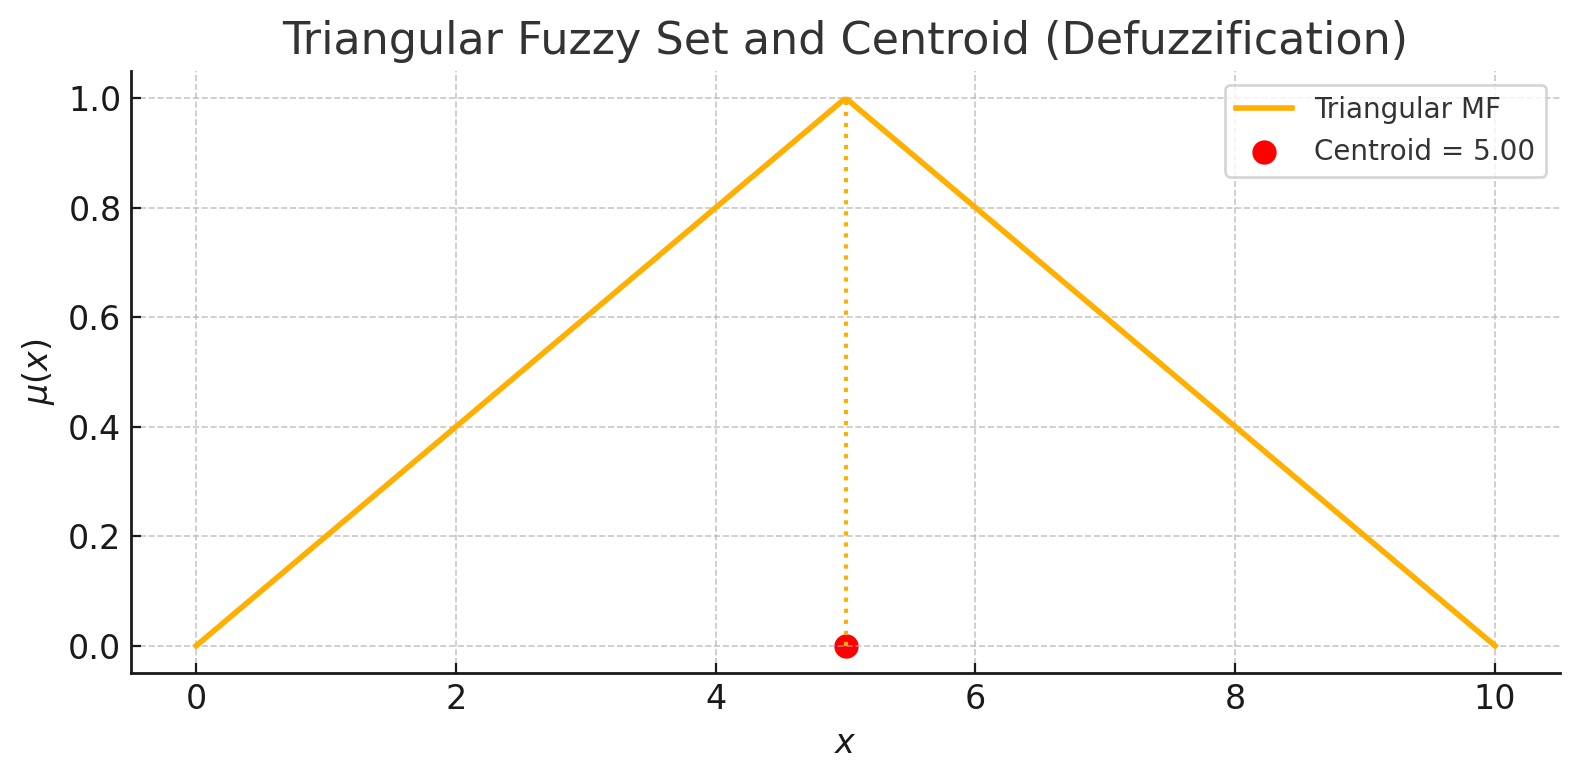
\includegraphics[width=\textwidth]{images/centroid_plot.png}
  \caption{Треугольное нечеткое множество и центр тяжести дефаззификации}
  \label{fig:centroid_defuzz}
\end{figure}

Для обучения нейро-нечетких систем используются методы настройки
весов \(w_{ij}\) и параметров функций принадлежности:
\begin{itemize}
  \item алгоритм обратного распространения ошибки (градиент первого порядка)~[4],
  \item метод Бройдена–Флетчера–Гольфарба–Шэнно (градиент второго порядка)~[3],
  \item эволюционные стратегии случайного поиска~[35].
\end{itemize}

Хотя увеличение числа обучаемых параметров повышает риск переобучения и
снижает интерпретируемость~[4], нейро-нечеткие системы демонстрируют высокую
эффективность при моделировании сложных процессов и интеллектуальном
анализе данных~[3,33].


\subsubsection{Методы нечёткого вывода}

\paragraph{1. Постановка задачи и основное определение}
Рассмотрим лингвистическую модель, состоящую из множества нечётких правил MISO-структуры:
\begin{equation}
  R_k:\quad
  \text{Если }x_1\in A_{1k}\wedge\cdots\wedge x_n\in A_{nk},\quad
  \text{то }y\in B_k,
  \label{eq:rule_general}
\end{equation}
где $A_{ik}\subseteq X_i, B_k\subseteq Y$ — нечёткие множества,
определённые функциями принадлежности
$\mu_{A_{ik}}:X_i\to[0,1]$, $\mu_{B_k}:Y\to[0,1]$.
Область входов: $\mathbf{x}=(x_1,\dots,x_n)\in X_1\times\cdots\times X_n=:X$.

\begin{definition}
Нечёткое отношение $R_k\subseteq X\times Y$ задаётся функцией
$$
  \mu_{R_k}(\mathbf{x},y)
  = I\bigl(\mu_{A_{1k}}(x_1),\dots,\mu_{A_{nk}}(x_n);\;\mu_{B_k}(y)\bigr),
$$
где $I:[0,1]^{n+1}\to[0,1]$ — неоднозначный импликатор, задающий связь
между степенями истинности посылок и заключения.
\end{definition}

\paragraph{2. Этапы классического вывода}
Нечёткий вывод традиционно проходит следующие этапы:

\begin{enumerate}
  \item \emph{Фаззификация входов.}
    Каждый числовой вход $x_i$ подвергается фаззификации:
    определяется вектор степеней
    $$
      (\mu_{A_{i1}}(x_i), \,\ldots, \,\mu_{A_{iN}}(x_i))
      \in [0,1]^N.
    $$
    Это позволяет перейти от точечного значения к распределению принадлежности.

  \item \emph{Активация правил.}
    Для каждого правила $R_k$ вычисляется степень активации
    \begin{equation}
      \alpha_k
      = T\bigl(\mu_{A_{1k}}(x_1),\dots,\mu_{A_{nk}}(x_n)\bigr),
      \label{eq:activation}
    \end{equation}
    где $T:[0,1]^n\to[0,1]$ — t-норма (обычно $\min$ или $\prod$).

  \item \emph{Инференция (применение импликации).}
    Применение импликатора $I$ даёт выходное нечеткое множество
    \begin{equation}
      \mu_{B'_k}(y)
      = I\bigl(\alpha_k,\mu_{B_k}(y)\bigr).
      \label{eq:inference}
    \end{equation}
    Наиболее часто используется
    $$
      \mu_{B'_k}(y)=\min\{\alpha_k,\mu_{B_k}(y)\}\quad(\text{Mamdani}),
    $$
    либо
    $$
      \mu_{B'_k}(y)=\alpha_k\,\mu_{B_k}(y)\quad(\text{Larsen}).
    $$

  \item \emph{Агрегация и дефаззификация.}
  \begin{itemize}
    \item Агрегация: объединение результатов всех правил
    $$
      \mu_{B'}(y)
      = \max_{1\le k\le N}\mu_{B'_k}(y).
    $$
    \item Дефаззификация: переход к числовому результату,
    например, по центру тяжести:
    \begin{equation}
      y^*
      = \displaystyle\frac{\int_Y y\,\mu_{B'}(y)\,dy}{\int_Y\mu_{B'}(y)\,dy}.
      \label{eq:defuzz_centroid}
    \end{equation}
  \end{itemize}
\end{enumerate}

\paragraph{3. Популярные варианты импликаторов и t–норм}
Подходы отличаются выбором $T$ и $I$:\
\textbf{Mamdani (1974).} $T=\min$, $I=\min$.\\
\textbf{Larsen (1980).} $T=\min$, $I(a,b)=a\cdot b$.\\
\textbf{Sugeno (1985).} Использует аналитические функции $f_k(x)$; итог:
$y^*=\sum\alpha_k y_k/\sum\alpha_k$.\\
\textbf{Tsukamoto (1979).} Монотонные функции для дефаззификации.

\paragraph{4. Доказательство полиномиальной сложности}
\begin{proof}
В классическом композиционном правиле необходимо проводить
максимум по всем комбинациям входов, что даёт $O(m^n)$ при $m$
уровнях фаззификации. В многоэтапном подходе каждая активация
\eqref{eq:activation} — $O(n)$, инференция \eqref{eq:inference} — $O(1)$,
агрегация — $O(N)$, дефаззификация — $O(m)$. Итого $O(n+N+m)$,
что полиномиально.
\end{proof}

\begin{figure}[h!]
  \centering
  \begin{tikzpicture}[scale=2.5,>=Stealth]
    \node at (-0.5,2.2){\textbf{Импликации}};
    \draw[->,ultra thick] (0,2) -- (1,2) node[midway,above]{\Large $\min$};
    \node at (1.2,2){\small Mamdani};
    \draw[->,ultra thick] (0,1) -- (1,1) node[midway,above]{\Large $\times$};
    \node at (1.2,1){\small Larsen};
  \end{tikzpicture}
  \caption{Увеличенный масштаб: минимум и произведение
    для иллюстрации импликаций.}
  \label{fig:implications_large2}
\end{figure}

\subsection{Нечёткая степень истинности}

Нечёткая степень истинности (НCИ) раскрывает степень соответствия одного нечёткого высказывания другому, выходя за рамки классического бивалентного анализа. Её важность обусловлена тем, что во множестве прикладных задач (управление, диагностика, обработка естественного языка) оценки носят нечёткий характер и требуют гибких мер сравнения.

\begin{definition}
Пусть $X$ — базовое множество, и даны два нечётких множества
\[
A = \{\mu_A(x)/x\mid x\in X\},\qquad
A' = \{\mu_{A'}(x)/x\mid x\in X\}.
\]
Нечёткой степенью истинности $A$ относительно $A'$ называют нечёткое множество
\(\CP(A,A')\subseteq[0,1]\) с функцией принадлежности
\begin{equation}\label{eq:degree_def_full}
\mu_{\CP(A,A')}(t)
=
\begin{cases}
\displaystyle
\sup_{\,x:\,\mu_A(x)=t}\,\mu_{A'}(x),
& \text{если }\{x\mid\mu_A(x)=t\}\neq\varnothing,\\[1em]
0,&\text{иначе}.
\end{cases}
\end{equation}
\end{definition}

Из определения сразу вытекает, что функция $\mu_{\CP(A,A')}(t)$ содержит всю информацию о «пересечении» уровневых множеств $A$ и $A'$.

\paragraph{Свойство монотонности t-нормы.}  
Пусть $T\colon[0,1]^2\to[0,1]$ — любая t-норма. Тогда по определению её монотонности для любых $u',u,v',v\in[0,1]$ из
\[
u'\le u,\quad v'\le v
\]
вытекает
\begin{equation}\label{eq:tnorm_monotonicity}
T(u',v') \;\le\; T(u,v).
\end{equation}

\begin{figure}[h]
  \centering
  \begin{tikzpicture}
    \pgfmathsetmacro{\cOne}{0.5}
    \pgfmathsetmacro{\sigmaOne}{0.1}
    \pgfmathsetmacro{\cTwo}{0.6}
    \pgfmathsetmacro{\sigmaTwo}{0.15}
    \begin{axis}[
      width=0.75\textwidth,
      domain=0:1,
      samples=200,
      xlabel={$x$}, ylabel={$\mu(x)$},
      grid=major,
      ymin=0, ymax=1,
      xtick=\empty,
      ytick={0,1},
      axis x line=bottom,
      axis y line=left,
      legend style={
        at={(0.98,0.98)},
        anchor=north east,
        font=\scriptsize,
        draw=black,
        inner sep=2pt,
        nodes={scale=0.8, transform shape}
      }
    ]
      \addplot[smooth, thick, blue]
        {exp(-((x-\cOne)^2)/(2*(\sigmaOne)^2))};
      \addplot[smooth, dashed, red]
        {exp(-((x-\cTwo)^2)/(2*(\sigmaTwo)^2))};
      \legend{
        $\displaystyle\mu_A(x)=\exp\!\Bigl(-\tfrac{(x-c_1)^2}{2\,\sigma_1^2}\Bigr)$,%
        $\displaystyle\mu_{A'}(x)=\exp\!\Bigl(-\tfrac{(x-c_2)^2}{2\,\sigma_2^2}\Bigr)$
      }
    \end{axis}
  \end{tikzpicture}
  \caption{Гауссовские функции принадлежности.}
\end{figure}

\paragraph{Аналитическое выражение при гауссовских функциях.}  
Пусть
\[
\mu_A(x)=\exp\!\bigl(-\tfrac{(x-a_1)^2}{2b_1^2}\bigr),\quad
\mu_{A'}(x)=\exp\!\bigl(-\tfrac{(x-a_2)^2}{2b_2^2}\bigr).
\]
Из \eqref{eq:degree_def_full} вытекает
\[
x = a_1 \pm b_1\sqrt{-2\ln t},
\]
а затем
\begin{equation}\label{eq:degree_gauss_full}
\mu_{\CP(A,A')}(t)
=
\max_{\pm}
\exp\!\Bigl\{-\tfrac{\bigl(a_1\pm b_1\sqrt{-2\ln t}-a_2\bigr)^2}{2b_2^2}\Bigr\}.
\end{equation}

\paragraph{Экстремальные точки.}  
Для поиска экстремума $\mu_{\CP}(t)$ находят производную:
\[
\mu'_{\CP}(t)
=
\Bigl(\pm b_1\,(a_1\pm b_1\sqrt{-2\ln t}-a_2)\Bigr)
\bigl(b_2^2\,t\,\sqrt{-2\ln t}\bigr)^{-1}
\exp\!\Bigl\{-\tfrac{(a_1\pm b_1\sqrt{-2\ln t}-a_2)^2}{2b_2^2}\Bigr\}.
\]
Приравнивая к нулю, получаем
\[
t = \exp\!\Bigl(-\tfrac{(a_2-a_1)^2}{2b_1^2}\Bigr),
\]
что соответствует единственному локальному максимуму.


\paragraph{Числовые меры.}  
Из $\mu_{\CP(A,A')}(t)$ определяют две основные меры:
\begin{align}
\Pi(A,A') &= \sup_{t\in[0,1]}\mu_{\CP(A,A')}(t), 
&\text{(мера возможности)},\\
N(A,A') &= 1 - \sup\{t\mid\mu_{\CP(A,A')}(t)=0\},
&\text{(мера необходимости)}.
\end{align}

\paragraph{Дискретный численный пример.}  
Пусть $X=\{x_1,x_2,x_3\}$ и
\[
\begin{aligned}
\mu_A(x_1)&=0.2,& \mu_{A'}(x_1)&=0.1,\\
\mu_A(x_2)&=0.5,& \mu_{A'}(x_2)&=0.6,\\
\mu_A(x_3)&=0.9,& \mu_{A'}(x_3)&=0.8.
\end{aligned}
\]
Тогда
\[
\mu_{\CP(A,A')}(0.2)=0.1,\quad
\mu_{\CP(A,A')}(0.5)=0.6,\quad
\mu_{\CP(A,A')}(0.9)=0.8,
\]
а для остальных $t$ — ноль.

\begin{figure}[h]
\centering
\begin{tikzpicture}
  \begin{axis}[
    width=0.8\textwidth,
    xlabel={$t$}, ylabel={$\mu_{\CP}(t)$},
    grid=major,
    ymin=0,ymax=1,xmin=0,xmax=1]
    \addplot[mark=none,] coordinates {(0,0) (0.2,0.1) (0.5,0.6) (0.9,0.8) (1,0)};
    \addplot[only marks] coordinates {(0.2,0.1) (0.5,0.6) (0.9,0.8)};
  \end{axis}
\end{tikzpicture}
\caption{Ступенчатая функция $\mu_{\CP(A,A')}(t)$ для дискретного примера.}
\end{figure}

\subsection{Нечёткое значение истинности}

Лингвистический подход трактует истинность как переменную
\[
\langle\beta,\,T,\,X,\,G,\,M\rangle,
\]
где $\beta=\text{«истинность»}$, $T$ — совокупность термов, $X=[0,1]$, $G$ — модификаторы, $M$ — функции принадлежности.

\begin{figure}[h]
  \centering
  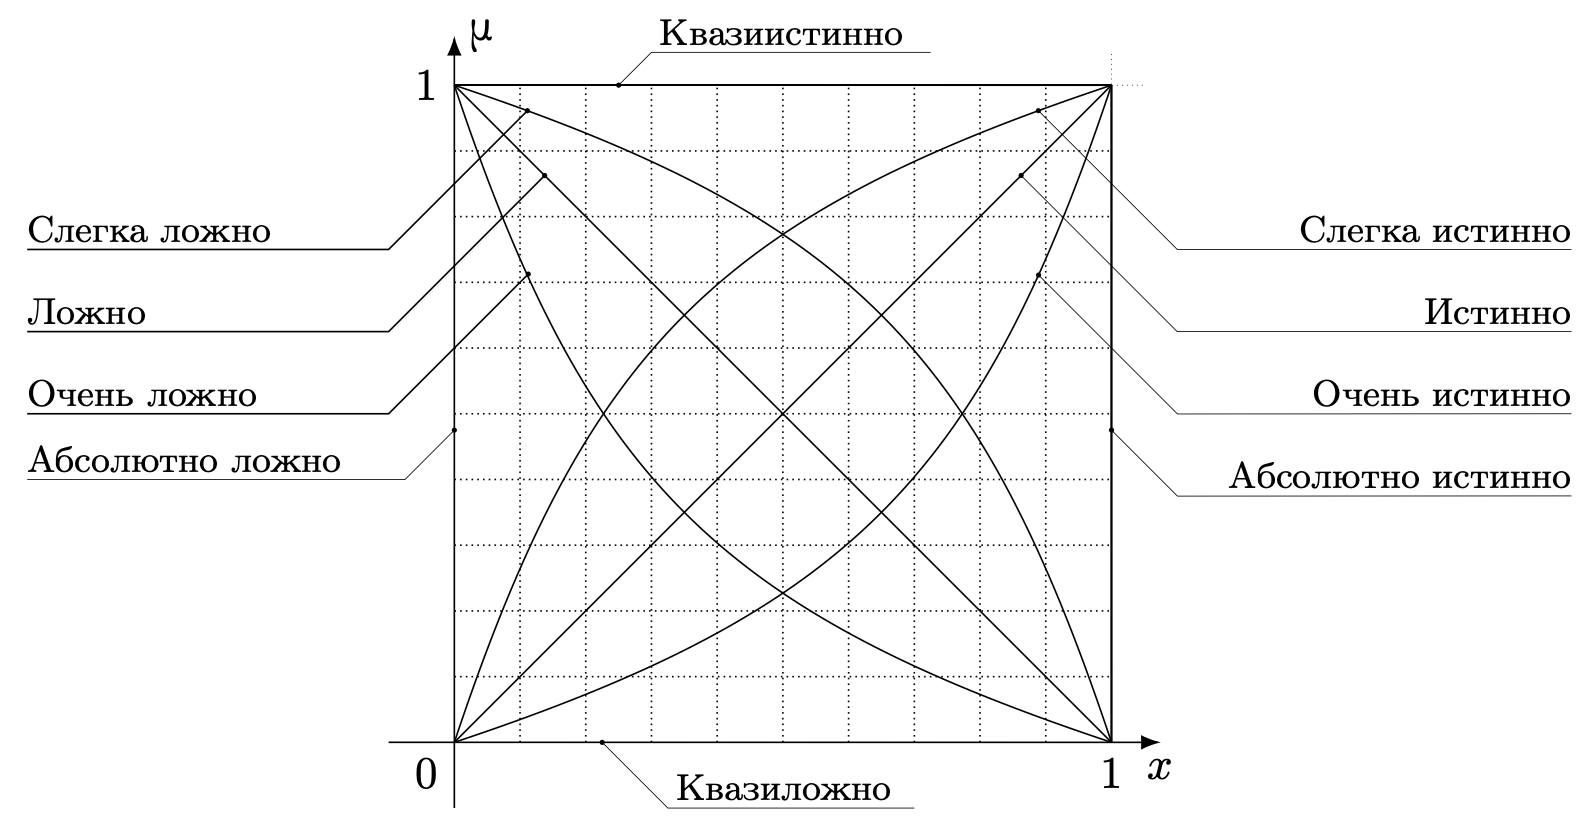
\includegraphics[width=\textwidth]{images/нечеткая истинность.png}
  \caption{Треугольное нечеткое множество и центр тяжести дефаззификации}
  \label{fig:centroid_defuzz}
\end{figure}

\begin{itemize}
  \item $\beta$ — название переменной («истинность»);
  \item $T = \{\text{абсолютно ложно, очень ложно, слегка ложно, ложно,\\
         квазиложно, квазиистинно, истинно, слегка истинно, очень истинно, абсолютно истинно}\}$
        — множество термов;
  \item $X = [0,1]$ — область значений лингвистической переменной;
  \item $G$ — синтаксическая процедура построения составных термов;
  \item $M$ — семантическая процедура, задающая функции принадлежности.
\end{itemize}

\paragraph{Примеры функций принадлежности термов.}
\[
\begin{aligned}
M[\text{«истинно»}](t)&=t,&
M[\text{«слегка истинно»}](t)&=\sqrt{t},\\
M[\text{«очень истинно»}](t)&=t^2,&
M[\text{«абсолютно истинно»}](t)&=
\begin{cases}1,&t=1,\\0,&t<1,\end{cases}\\
M[\text{«ложно»}](t)&=1-t,&
M[\text{«слегка ложно»}](t)&=\sqrt{1-t},\\
M[\text{«очень ложно»}](t)&=(1-t)^2,&
M[\text{«абсолютно ложно»}"](t)&=
\begin{cases}1,&t=0,\\0,&t>0.\end{cases}
\end{aligned}
\]
\begin{figure}[h]
\centering
\begin{tikzpicture}
  \begin{axis}[
    width=0.6\textwidth,
    xlabel={$t$}, ylabel={$\mu$},
    grid=major,
    legend style={at={(1.02,1)},anchor=north west}]
    \addplot {x}; \addlegendentry{истинно}
    \addplot {sqrt(x)}; \addlegendentry{слегка истинно}
    \addplot {x^2}; \addlegendentry{очень истинно}
    \addplot {1-x}; \addlegendentry{ложно}
    \addplot {sqrt(1-x)}; \addlegendentry{слегка ложно}
    \addplot {(1-x)^2}; \addlegendentry{очень ложно}
  \end{axis}
\end{tikzpicture}
\caption{Функции принадлежности лингвистических термов истинности.}
\end{figure}
\paragraph{Лингвистическая интерпретация.}  
\begin{itemize}
  \item «абсолютно истинно», если $\mu_{\CP(A,A')}(t)=1$ на всём диапазоне;
  \item «квазиистинно», если функция близка к 1 на широком промежутке уровней;
  \item «квазиложно», если функция близка к 0 на большинстве уровней;
  \item «абсолютно ложно», если не совпадает ни в одной точке.
\end{itemize}

\paragraph{Дополнительные замечания.}
\begin{itemize}
  \item Методы оценки степени истинности можно расширить на интуитивно-нечёткие множества и другие обобщения.
  \item Для сложных систем часто применяют численные методы приближённого вычисления $\mu_{\CP}(t)$ на дискретной сетке.
  \item Сравнение различных t-норм и импликаций позволяет настраивать «строгость» выводов в нечётких системах.
\end{itemize}
% \subsubsection{Нечёткое значение истинности}
%
% \paragraph{1. Определение и мотивация}
% Числовое значение истинности
% \(\tau_{A/A'}\in[0,1]\)
% задаётся как:
% \begin{equation}
%   \tau_{A/A'}
%   = \sup_{x\in X}\min\{\mu_A(x),\,\mu_{A'}(x)\}.
%   \label{eq:tau_def3b}
% \end{equation}
% Оно отражает максимальную степень одновременного
% "принадлежания" $x$ множествам $A$ и $A'$.
%
% \paragraph{2. Подробное доказательство свойств}
% \begin{theorem}
% Величина $\tau_{A/A'}$:\
% (1) равна 1 тогда и только тогда, когда
% $\mu_A(x)\le\mu_{A'}(x)$ при всех $x$;\
% (2) равна 0 тогда и только тогда,
% когда $\min\{\mu_A(x),\mu_{A'}(x)\}=0$ для всех $x$;\
% (3) монотонна:
% $A_1\subseteq A_2\implies \tau_{A_1/A'}\le \tau_{A_2/A'}$.
% \end{theorem}
%
% \begin{proof}
% Из определения \eqref{eq:tau_def3b} следует,
% что максимум достигается при $x$, где
% $\min(\mu_A,\mu_{A'})$ максимален. Для (1):
% если $\mu_A(x)\le\mu_{A'}(x)$, то
% $\min(\mu_A,\mu_{A'})=\mu_A$ и
% $\sup_x\mu_A(x)=1$. Обратное — аналогично.
% Для (2): $\min(\mu_A,\mu_{A'})=0$ на всех $x$.
% Монотонность — из неубывания $\mu_{A_1}\le\mu_{A_2}$.
% \end{proof}
%
% \begin{figure}[h!]
%   \centering
%   \begin{tikzpicture}[scale=2.5,>=Stealth]
%     \draw[->] (0,0)--(4,0) node[right]{$x$};
%     \draw[->] (0,0)--(0,2) node[above]{$\mu$};
%     \draw[thick,blue,domain=0:4,samples=100]
%       plot(\x,{exp(-((\x-1.3)^2)/0.8)});
%     \node at (1.3,1.6){\footnotesize $\mu_A(x)$};
%     \draw[thick,red,domain=0:4,samples=100]
%       plot(\x,{exp(-((\x-2.7)^2)/1.1)});
%     \node at (2.7,1.1){\footnotesize $\mu_{A'}(x)$};
%     \fill[gray,opacity=0.4]
%       plot[domain=1.6:2.4] (\x,{min(exp(-((\x-1.3)^2)/0.8),exp(-((\x-2.7)^2)/1.1))})
%       -- (2.4,0) -- (1.6,0) -- cycle;
%     \node at (2.0,0.5){\small перекрытие};
%   \end{tikzpicture}
%   \caption{Увеличенный пример: область перекрытия
%     для численного $\tau_{A/A'}$.}
%   \label{fig:tau_enlarged2}
% \end{figure}
%
% Логика, опирающаяся на концепцию нечеткой истинности, обычно именуется лингвистической. 
% В рамках этого подхода «нечеткая истинность» рассматривается как лингвистическая переменная, задаваемая пятёркой
% \[
% \langle \beta,\, T,\, X,\, G,\, M\rangle,
% \]
% где
% \begin{itemize}
%   \item $\beta$ — название переменной («истинность»);
%   \item $T = \{\text{абсолютно ложно, очень ложно, слегка ложно, ложно,\\
%          квазиложно, квазиистинно, истинно, слегка истинно, очень истинно, абсолютно истинно}\}$
%         — множество термов;
%   \item $X = [0,1]$ — область значений лингвистической переменной;
%   \item $G$ — синтаксическая процедура построения составных термов;
%   \item $M$ — семантическая процедура, задающая функции принадлежности.
% \end{itemize}
% \begin{figure}[h]
%   \centering
%   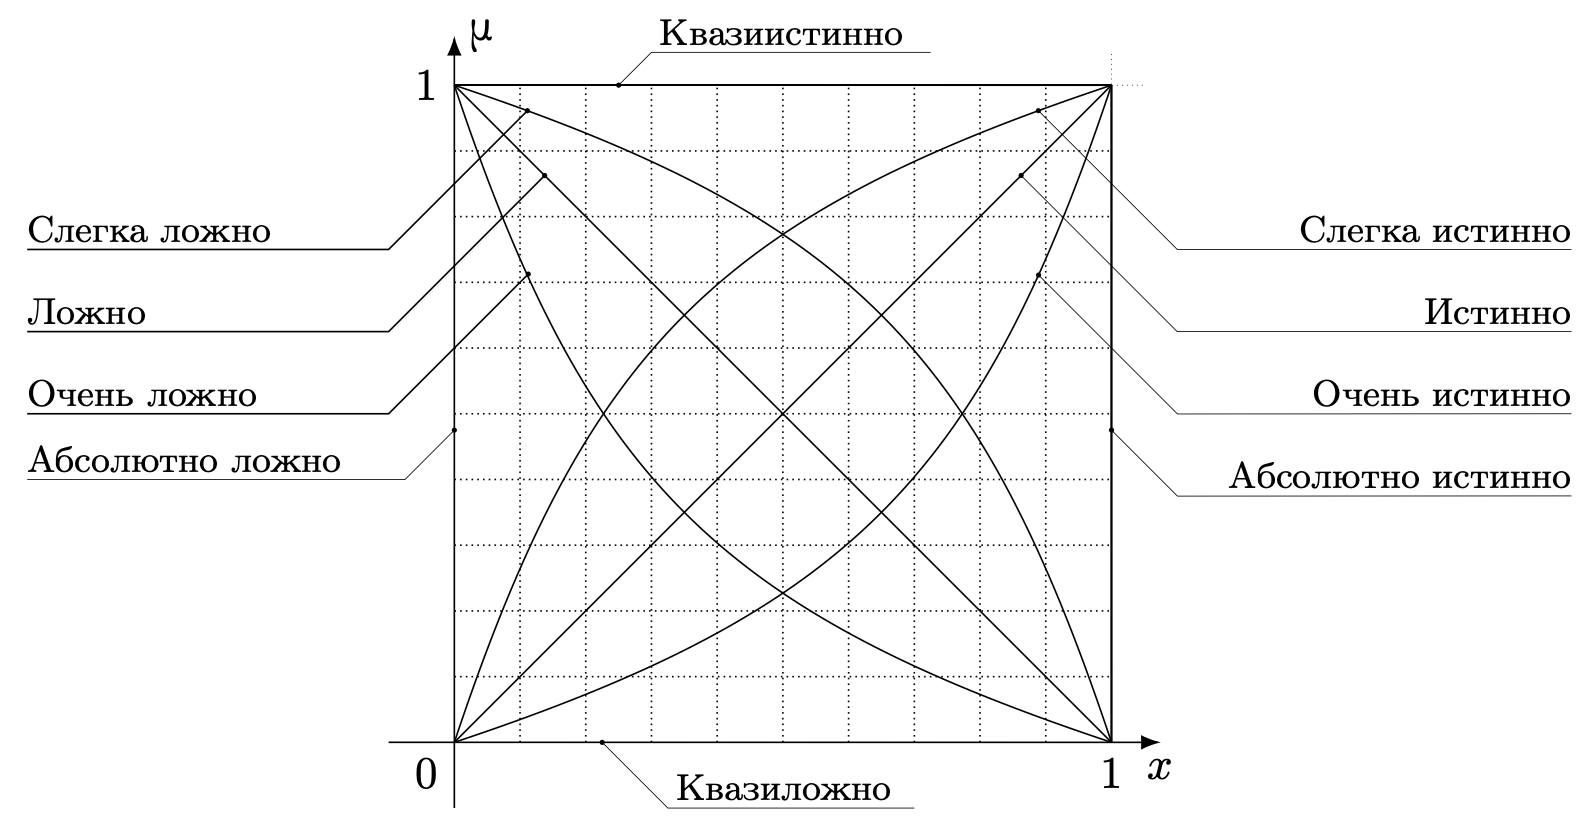
\includegraphics[width=\textwidth]{images/нечеткая истинность.png}
%   \caption{Треугольное нечеткое множество и центр тяжести дефаззификации}
%   \label{fig:centroid_defuzz}
% \end{figure}
% \subsubsection{Методы нечёткого вывода}
% \subsubsection{Нечёткое значение истинности}
% \subsubsection{Нечёткая степень истинности}

% \subsection{Проблемы исходных данных в задачах машинного обучения}
% \subsubsection{Размасштабированность и гетерогенность признаков}
% \subsubsection{Шум, выбросы и пропуски}
% \subsubsection{Несбалансированность классов}
%
% \newpage
%
% \subsection{Обзор инструментальных средств}
% \subsubsection{Выбор языка программирования: Python}
% \subsubsection{Использование GPU: CUDA и PyTorch}
% Лингвистическая логика на основе нечеткой истинности
\subsection{Обзор инструментальных средств}
\label{sec:tools}

\subsubsection{Выбор языка программирования: Python}
\label{sec:tools_python}

Python — язык высокого уровня с лаконичным синтаксисом. Основные преимущества:
\begin{itemize}
  \item Обширная экосистема научных библиотек: \texttt{NumPy}, \texttt{SciPy}, \\ \texttt{Pandas}, \texttt{Matplotlib}
  \item Фреймворки для машинного обучения: \texttt{scikit-learn}, \texttt{TensorFlow}, \\ \texttt{PyTorch}
  \item Быстрое прототипирование в Jupyter;
  \item Большое сообщество и документация.
\end{itemize}

\subsection{Архитектура и оптимизация GPU для обучения нейронных сетей}
\label{ssec:gpu_architecture}

Графические процессоры (GPU) изначально создавались для рендеринга трёхмерной графики, где требовалось одновременно обрабатывать миллионы пикселей. Однако, когда стало ясно, что обучение глубоких нейросетей сводится к повторению единотипных операций над большими массивами чисел, архитектура GPU оказалась почти идеальной. В отличие от CPU с его несколькими быстро работающими ядрами и громоздкой системой предсказания ветвлений, GPU использует сотни или тысячи упрощённых ядер, которые синхронно выполняют одну и ту же инструкцию над разными данными.   

Для понимания того, как они отличаются, достаточно вспомнить, что современные серверные CPU обычно имеют 8–64 полноценных ядра, каждое из которых оснащено суперскалярным исполнителем, многоуровневой кэш-иерархией (L1–L3) и сложной системой предсказания переходов. Такая структура хорошо подходит для разнородных задач — ветвящихся алгоритмов, многозадачности, работы с нерегулярными структурами данных, но она не способна раскрутить более чем десятки параллельных потоков без значительного роста стоимости и энергопотребления.  

GPU же строятся по принципу «массированного параллелизма»: независимые арифметические блоки объединяются в стриминговые мультипроцессоры (Streaming Multiprocessors, SM), а SM, в свою очередь, умножаются до сотен штук на кристалле. Потоки группируются в «warps» (в NVIDIA) или «wavefronts» (в AMD), и все нити в такой группе исполняют одну и ту же инструкцию. Внутри SM есть быстрое локальное хранилище (shared memory) и регистры, что позволяет координировать взаимодействие потоков с минимальной задержкой.  

Память GPU организована в несколько уровней:  
\begin{itemize}  
  \item \emph{Глобальная память (VRAM)} на основе GDDR6 или HBM2/3 обеспечивает пропускную способность до нескольких терабайт в секунду, но обладает заметной латентностью.  
  \item \emph{Кэш уровня L2} объединяет доступы от всех SM и снижает количество обращений к глобальной памяти.  
  \item \emph{Разделяемая память} внутри каждого SM и \emph{регистры} обеспечивают сверхнизкую латентность при обмене данными между соседними тредами.  
\end{itemize}  

Ключевым усовершенствованием последних поколений стало появление тензорных ядер (Tensor Cores), рассчитанных на смешанную точность (обычно FP16/FP32 или BF16). Они позволяют выполнять матричные умножения $4\times4$ или даже $16\times16$ за один такт, что даёт дополнительный прирост производительности в несколько раз при сохранении приемлемой точности сходимости.  

С точки зрения ПО разработчики используют платформы CUDA (NVIDIA) или HIP (AMD), где вся работа разбивается на:  
\begin{itemize}  
  \item \textbf{Запуск кернелов} — небольших программ, которые выполняются на тысячах потоков одновременно.  
  \item \textbf{Асинхронные копирования} (CUDA MemcpyAsync) — перекрытие передачи данных между CPU и GPU с вычислениями, чтобы видеокарта не простаивала.  
  \item \textbf{Стримы и графы задач} — механизм группировки операций для минимизации накладных расходов вызова ядра.  
  \item \textbf{Kernel Fusion} — объединение последовательных операций в единый кернел, позволяющее сократить число обращений к глобальной памяти.  
\end{itemize}  

На практике обучение крупных нейросетей нередко разбивают на две части:  
\begin{enumerate}  
  \item Предобработка, аугментация и загрузка данных (I/O, трансформации) выполняются на CPU, где быстрее работают ветвления и системные вызовы.  
  \item Основной проход (forward/backward) и обновление параметров — на GPU, где тысячи ядер решают одинаковые подзадачи над матрицами и тензорами.  
\end{enumerate}  

Визуализация профилей реальных задач показывает, что современные ускорители типа NVIDIA A100 обеспечивают до 1–1.5 PFLOPS в смешанной точности при потреблении порядка 300 Вт, тогда как эквивалентная нагрузка на серверный CPU (Intel Xeon) даст лишь пару сотен GFLOPS при схожем энергопотреблении. Это объясняет, почему GPU остаются ключевым ресурсом для дата-центров машинного обучения.  

Конечно, у GPU есть и ограничения:  
\begin{itemize}  
  \item \textbf{Ограниченный объём VRAM}. Модели типа GPT-3 XXL могут не помещаться на одной карте, требуя шардирования по нескольким GPU.  
  \item \textbf{Высокая латентность случайных доступов} к памяти усложняет нерегулярные вычисления и динамические графы.  
  \item \textbf{Накладные расходы} на передачу данных по PCIe/NVLink (несколько миллисекунд при больших объёмах).  
  \item \textbf{Сложность отладки} параллельных алгоритмов и профилирования (нужны специальные инструменты: Nsight, rocProfiler).  
\end{itemize}  

В ближайшие годы мы увидим всё более плотную интеграцию CPU и GPU в едином корпусе (NVIDIA Grace, AMD Instinct CDNA), а также рост популярности альтернативных ускорителей — TPU от Google, FPGA и экспериментальных оптических и нейроморфных чипов. Эти гибридные решения позволят сократить задержки передачи данных и ещё более повысить эффективность распределённых систем глубокого обучения.  


\subsubsection{Использование GPU: CUDA и PyTorch}
\label{sec:tools_gpu}

\paragraph{Модель программирования CUDA}
Программист описывает kernel-функции, которые запускаются параллельно. Пример сложения двух векторов:

\begin{lstlisting}[language=C,caption={CUDA: сложение векторов},label={lst:cuda_vecadd}]
__global__ void vecAdd(const float *A, const float *B, float *C, int N) {
    int i = blockIdx.x * blockDim.x + threadIdx.x;
    if (i < N) {
        C[i] = A[i] + B[i];
    }
}

float *d_A, *d_B, *d_C;
cudaMalloc(&d_A, N * sizeof(float));
cudaMalloc(&d_B, N * sizeof(float));
cudaMalloc(&d_C, N * sizeof(float));
cudaMemcpy(d_A, h_A, N * sizeof(float), cudaMemcpyHostToDevice);

int blockSize = 256;
int gridSize  = (N + blockSize - 1) / blockSize;
vecAdd<<<gridSize, blockSize>>>(d_A, d_B, d_C, N);

cudaMemcpy(h_C, d_C, N * sizeof(float), cudaMemcpyDeviceToHost);
\end{lstlisting}

\paragraph{Оптимизации для CUDA}
\begin{itemize}
  \item Coalesced memory access: чтение подряд идущих адресов одним warp\;
  \item Shared memory для уменьшения обращений к глобальной памяти\;
  \item Асинхронное копирование и стримы (\texttt{cudaMemcpyAsync}, \texttt{cudaStream}) для перекрытия вычислений и передачи данных.
\end{itemize}

\paragraph{PyTorch и GPU}
PyTorch позволяет легко переносить тензоры на устройство и выполнять вычисления:

\begin{lstlisting}[language=Python,caption={PyTorch: базовые операции на GPU},label={lst:torch_gpu}]
import torch

t = torch.randn(1024, 1024, device='cuda')

y = torch.mm(t, t)

x = torch.tensor([1., 2., 3.], device='cuda', requires_grad=True)
y = x.pow(2).sum()
y.backward()
print(x.grad)  # tensor([2., 4., 6.], device='cuda:0')
\end{lstlisting}

\paragraph{Сравнение библиотек}
\textbf{TensorFlow} (статический граф):
\begin{lstlisting}[language=Python,caption={TensorFlow: определение и запуск функции},label={lst:tf}]
import tensorflow as tf

@tf.function
def fwd(x):
    return tf.matmul(x, x)

x = tf.random.normal((1024, 1024))
y = fwd(x)
\end{lstlisting}

\textbf{JAX} (JIT и векторизация):
\begin{lstlisting}[language=Python,caption={JAX: JIT-компиляция и градиент},label={lst:jax}]
import jax.numpy as jnp
from jax import jit, grad

@jit
def f(x):
    return jnp.dot(x, x)

res = f(jnp.ones((1024, 1024)))
g = grad(lambda m: jnp.sum(m**2))(jnp.ones((3,)))
\end{lstlisting}

\textbf{MXNet} (Gluon API):
\begin{lstlisting}[language=Python,caption={MXNet: dot-операция на GPU},label={lst:mxnet}]
from mxnet import nd, gpu

x = nd.random.normal(shape=(1024,1024), ctx=gpu())
w = nd.random.normal(shape=(1024,1024), ctx=gpu())
y = nd.dot(x, w)
\end{lstlisting}

PyTorch выделяется динамическим графом и удобством отладки, TensorFlow — оптимизацией статических моделей, JAX — простотой JIT и векторизации, MXNet — гибкостью Gluon API.

\subsection{Методы предварительной обработки и улучшения данных}

В современных задачах машинного обучения и анализа данных качество результатов во многом зависит от корректности и информативности исходных признаков. Процесс \emph{предварительной обработки} (preprocessing) включает в себя целый набор операций, направленных на приведение данных к удобному для моделей виду, снижение шумов и балансировку выборки. Ниже приведены три ключевых группы методов: масштабирование, синтетическое дополнение редких классов и работа с выбросами. Для каждой группы описаны цели, основные подходы, преимущества и ограничения, а также приведены примеры формул и кода на Python.

% ----------------------------------------
\subsubsection{Масштабирование}
\label{sec:scaling}

\paragraph{Зачем нужно масштабирование?}  
Многие алгоритмы (например, методы на основе евклидова расстояния или градиентного спуска) чувствительны к масштабу признаков. Если один признак принимает значения от 0 до 1, а другой — от \(10^3\) до \(10^6\), модель будет «смотреть» в первую очередь на крупномасштабный признак. Кроме того, плохая масштабировка может замедлять сходимость оптимизации.

\paragraph{Основные методы}
\begin{itemize}
  \item \textbf{Min–Max нормализация:}  
    \[
      x' = \frac{x - x_{\min}}{x_{\max} - x_{\min}},
      \quad x'\in[0,1].
    \]
    \emph{Плюсы:} сохраняет форму распределения, легко интерпретировать.  
    \emph{Минусы:} чувствительна к выбросам, требует знания глобальных минимумов и максимумов.
    
  \item \textbf{Z-преобразование (Standardization):}  
    \[
      x' = \frac{x - \mu}{\sigma},
      \quad \mu = \frac{1}{n}\sum_i x_i,\;
      \sigma = \sqrt{\frac{1}{n}\sum_i (x_i - \mu)^2}.
    \]
    \emph{Плюсы:} приводит данные к нулевому среднему и единичному стандартному отклонению, устойчиво при небольших выбросах.  
    \emph{Минусы:} всё ещё может страдать от сильных выбросов.
    
  \item \textbf{Десятичное масштабирование:}  
    \[
      x' = \frac{x}{10^j},\quad
      j = \left\lceil \log_{10}\bigl(\max_i |x_i|\bigr)\right\rceil.
    \]
    \emph{Плюсы:} просто реализуется, гарантирует \(|x'|<1\).  
    \emph{Минусы:} не выравнивает распределение, работает только с десятичной шкалой.
    
  \item \textbf{Робастное масштабирование:}  
    \[
      x' = \frac{x - \mathrm{median}(x)}{\mathrm{IQR}(x)},
      \quad \mathrm{IQR} = Q_3 - Q_1.
    \]
    \emph{Плюсы:} устойчиво к выбросам.  
    \emph{Минусы:} требует расчёта квартилей, менее распространено.
\end{itemize}

\paragraph{Снижение размерности как частный случай}  
Иногда под «масштабированием» понимают удаление избыточных признаков.  
\begin{itemize}
  \item \emph{PCA} (метод главных компонент): решается собственная задача для ковариационной матрицы и берутся \(k\) ведущих компонент:
    \[
      X' = XW,\quad W = [v_1,\dots,v_k],\quad \Sigma v_i = \lambda_i v_i.
    \]
  \item \emph{LDA} (линейный дискриминантный анализ): максимизация отношения межклассовой и внутриклассовой дисперсии.
  \item Нелинейные методы \emph{t-SNE}, \emph{UMAP} — для визуализации в 2–3D.
\end{itemize}

\paragraph{Пример на Python}
\begin{lstlisting}[language=Python]
from sklearn.preprocessing import MinMaxScaler, StandardScaler
from sklearn.decomposition import PCA

mm = MinMaxScaler(feature_range=(0,1))
X_mm = mm.fit_transform(X)

std = StandardScaler()
X_std = std.fit_transform(X)

pca = PCA(n_components=2, random_state=42)
X_pca = pca.fit_transform(X_std)
\end{lstlisting}

% ----------------------------------------
\subsubsection{Синтетическое дополнение редких классов}
\label{sec:oversampling}

\paragraph{Почему важно дополнять редкие классы?}  
В случае сильного дисбаланса модель может «игнорировать» малочисленные классы, отказываться им уделять внимание и выдавать предсказания лишь для большинства. Синтетическое дополнение (oversampling) помогает сгладить этот эффект, повысить чувствительность к редким событиям и улучшить общую сбалансированность.

\paragraph{Методы синтеза}
\begin{enumerate}
  \item \textbf{SMOTE} (Synthetic Minority Over-sampling Technique):  
    Для каждой точки \(x_i\) класса-минорити выбирается один из \(k\) ближайших соседей \(x_{\rm nn}\) и синтезируется:
    \[
      x_{\rm new} = x_i + \delta\,(x_{\rm nn} - x_i),\quad \delta\in[0,1].
    \]
  \item \textbf{Borderline-SMOTE}:  
    Генерация новых примеров только в «пограничных» зонах, где редкий класс пересекается с мажорити.
  \item \textbf{ADASYN}:  
    Учитывает плотность объектов, создаёт больше синтетических точек там, где редкий класс особенно редок.
  \item \textbf{GAN-базированные методы}:  
    Обучают генератор/дискриминатор для создания правдоподобных новых образцов.
\end{enumerate}

\paragraph{Плюсы и минусы}
\begin{itemize}
  \item \emph{Плюсы:}  
    \begin{itemize}
      \item Сглаживает дисбаланс без потери информации.  
      \item Увеличивает объём обучающей выборки, что может улучшить регуляризацию.
    \end{itemize}
  \item \emph{Минусы:}  
    \begin{itemize}
      \item Риск переобучения на синтетических данных.  
      \item При сложном многомерном распределении могут появиться «ненатуральные» точки.
    \end{itemize}
\end{itemize}

\paragraph{Пример на Python}
\begin{lstlisting}[language=Python]
from imblearn.over_sampling import SMOTE

smote = SMOTE(sampling_strategy='minority', k_neighbors=5, random_state=42)
X_res, y_res = smote.fit_resample(X, y)
\end{lstlisting}

% ----------------------------------------
\subsubsection{Обнаружение и устранение выбросов}
\label{sec:outliers}

\paragraph{Зачем искать выбросы?}  
Выбросы могут искажать оценки параметров (среднее, дисперсию), влиять на обучение моделей и ухудшать обобщающую способность. При этом не все «экстремальные» значения — ошибки: порой это важные редкие события.

\paragraph{Методы обнаружения}
\begin{itemize}
  \item \textbf{Статистические критерии:}
    \begin{itemize}
      \begin{equation}
      \item Z-score: \(\displaystyle |z_i| > \tau\) (\(\tau\approx3\)).
      \item IQR-критерий: \(x < Q_1 - 1.5\,\mathrm{IQR}\) или \(x > Q_3 + 1.5\,\mathrm{IQR}\).
      \end{equation}
    \end{itemize}
  \item \textbf{Алгоритмические:}
    \begin{itemize}
      \item Isolation Forest: строит деревья, в которых «аномалии» изолируются быстрее.
      \item Local Outlier Factor: сравнивает плотность вокруг точки с плотностью у соседей.
      \item One-Class SVM: обучается только на «нормальных» данных и выявляет выбросы.
    \end{itemize}
\end{itemize}

\paragraph{Стратегии устранения}
\begin{itemize}
  \item \emph{Удаление:} простое отбрасывание аномальных строк.
  \item \emph{Замена:} подстановка медианы, моды или крайних значений.
  \item \emph{Капирование (capping):} обрезание выходящих за пределы значений до выбранных порогов.
\end{itemize}

\begin{table}[h]
\centering
\caption{Плюсы и минусы}
\label{tab:pros_cons}
\begin{tabularx}{\textwidth}{@{}>{\raggedright\arraybackslash}X>{\raggedright\arraybackslash}X@{}}
\toprule
\textbf{Плюсы} & \textbf{Минусы} \\
\midrule
Повышает надёжность статистических оценок. & Можно случайно удалить важные редкие события. \\
\addlinespace[0.5em]
Облегчает обучение моделей, снижает риск переобучения на шуме. & Сложно задать универсальные пороги для разных признаков. \\
\bottomrule
\end{tabularx}
\end{table}

\paragraph{Пример на Python}
\begin{lstlisting}[language=Python]
import numpy as np
from sklearn.ensemble import IsolationForest

z_scores = (X - X.mean(axis=0)) / X.std(axis=0)
mask = np.all(np.abs(z_scores) < 3, axis=1)
X_clean_z = X[mask]

iso = IsolationForest(contamination=0.05, random_state=0)
labels = iso.fit_predict(X)
X_clean_if = X[labels == 1]
\end{lstlisting}

% ----------------------------------------
% Конец раздела
% ----------------------------------------
% \subsection{Методы предварительной обработки и улучшения данных}
% \subsubsection{Масштабировани}
% \subsubsection{Синтетическое дополнение редких классов (SMOTE)}
% \subsubsection{Обнаружение и устранение выбросов}
%
\subsection{Инструменты и методы оптимизации гиперпараметров}
\label{sec:hyperparameter-optimization}

Под гиперпараметрами понимаются конфигурационные параметры модели или алгоритма, устанавливаемые до начала процесса обучения или инициализации и не обновляемые в процессе градиентного спуска или другого метода оптимизации. К классическим примерам относятся скорость обучения, глубина дерева решений, число скрытых слоёв нейросети и параметры регуляризации. Более того, в гибридных системах нейронно-нечеткой логики гиперпараметрами могут быть весовые коэффициенты правил нечеткого вывода, параметры функций принадлежности и пороги активации. Корректный подбор гиперпараметров напрямую влияет на качество работы модели, скорость её сходимости, устойчивость к переобучению и способность адаптироваться к сложным неопределённым условиям.

\subsubsection{Классические методы}

\paragraph{Перебор по сетке (Grid Search)}  
Пусть для каждого из \(k\) гиперпараметров задано дискретное множество \(P_i\), \(|P_i|=n_i\). Тогда полный перебор предполагает проверку всех комбинаций:
\begin{equation}
\mathcal{P} \;=\; P_1 \times P_2 \times \cdots \times P_k,
\qquad
|\mathcal{P}| \;=\; \prod_{i=1}^k n_i.
\label{eq:grid-search-size}
\end{equation}
\textbf{Плюсы:} простота реализации, гарантированное покрытие решётки.  
\textbf{Минусы:} экспоненциальный рост числа испытаний при увеличении \(k\) и \(n_i\).

\paragraph{Случайный поиск (Random Search)}  
При ограниченном бюджете \(N\) испытаний точки выбираются в гиперпространстве равномерно:
\begin{equation}
p_i^{(j)} \;\sim\; \mathcal{U}(a_i, b_i),
\quad j = 1,\dots,N.
\label{eq:random-search}
\end{equation}
\citet{bergstra2012random} показали, что при фиксированном \(N\) Random Search часто эффективнее Grid Search, так как распределяет усилия по более важным измерениям.

\subsubsection{Байесовская оптимизация}

Методы байесовской оптимизации строят суррогатную модель целевой функции
\(
f\colon \mathcal{X}\to\mathbb{R}
\)
на основе предыдущих наблюдений \(\mathcal{D}=\{(x_i, f(x_i))\}\) и используют функцию приобретения \(\alpha(x)\) для выбора следующей точки:
\begin{equation}
x_{n+1} = \arg\max_{x\in\mathcal{X}} \alpha\bigl(x;\,p(f\mid\mathcal{D})\bigr).
\label{eq:bayes-opt}
\end{equation}

\paragraph{Gaussian Process (GP)}  
Суррогатная модель задаётся процессом:
\begin{equation}
f(x)\sim\mathcal{GP}\bigl(m(x),\,k(x,x')\bigr),
\label{eq:gp-prior}
\end{equation}
где \(m(x)\) — функция среднего, \(k(x,x')\) — ковариационное ядро. По данным \(\mathcal{D}\) получают предсказание \(\mu_n(x)\) и неопределённость \(\sigma_n(x)\).

\paragraph{Функции приобретения}  
\begin{align}
\mathrm{EI}(x)
&= (f_{\min}-\mu_n(x))\,\Phi\bigl(Z\bigr)
+ \sigma_n(x)\,\phi\bigl(Z\bigr),
\quad Z = \frac{f_{\min}-\mu_n(x)}{\sigma_n(x)},
\label{eq:expected-improvement}\\
\mathrm{PI}(x)
&= \Phi\!\Bigl(\frac{f_{\min}-\mu_n(x)}{\sigma_n(x)}\Bigr),
\label{eq:probability-improvement}\\
\mathrm{UCB}(x)
&= \mu_n(x) - \kappa\,\sigma_n(x).
\label{eq:upper-conf-bound}
\end{align}

\subsubsection{Адаптивное распределение ресурсов}

\paragraph{Successive Halving}  
Все \(n\) конфигураций обучаются на малом бюджете \(r\), затем отбираются лучшие \(n/\eta\) и их обучают с бюджетом \(\eta r\), и так далее.

\paragraph{Hyperband / ASHA}  
Комбинирует Successive Halving с несколькими начальными бюджетами \(r_1, r_2, \dots, r_s\), что позволяет балансировать между шириной и глубиной поиска.

\subsubsection{Современные фреймворки}

\begin{itemize}
  \item \textbf{Optuna}. Основан на TPE (Tree-structured Parzen Estimator).
  \item \textbf{Hyperopt}. Реализует TPE и Random Search, конфигурируется через Python-словари.
  \item \textbf{Scikit-Optimize (skopt)}. Предоставляет \texttt{gp\_minimize},  \\
    \texttt{forest\_minimize}, \texttt{gbrt\_minimize}.
  \item \textbf{Ray Tune}. Распределённая оптимизация с поддержкой HyperOpt, BayesOpt, HyperBand.
  \item \textbf{SMAC}. Bayesian Optimization на основе Random Forest.
\end{itemize}

\subsubsection{Пример использования Optuna}

\begin{lstlisting}[language=Python]
import optuna

def objective(trial):
    lr = trial.suggest_loguniform('learning_rate', 1e-5, 1e-1)
    n_estimators = trial.suggest_int('n_estimators', 50, 500)
    score = train_and_evaluate(lr, n_estimators)
    return score

study = optuna.create_study(direction='minimize')
study.optimize(objective, n_trials=50)
\end{lstlisting}

\end{document}

\section{Проектирование программного обеспечения}

%==============================================================
%  Н Е Ч Ё Т К А Я   Л О Г И К А
%==============================================================

\subsection{Нечёткая логика}
%--------------------------------------------------------------
\subsubsection{Основные определения}

\begin{definition}
Нечёткое множество $A$ на универсуме $X$ задаётся функцией принадлежности
\begin{equation}
  \mu_A\colon X \longrightarrow [0,1],
  \label{eq:fuzzy_set_def}
\end{equation}
где значение $\mu_A(x)$ количественно отражает,
\emph{насколько} верно высказывание «$x$ принадлежит $A$»:
\[
  \mu_A(x)=
  \begin{cases}
    0          &\text{― точно не принадлежит},\\
    1          &\text{― принадлежит полностью},\\
    (0,1)      &\text{― принадлежит частично}.
  \end{cases}
\]
\end{definition}

\begin{definition}
Нечёткое множество $A$ называется
\emph{нормальным}, если существует хотя бы одна точка
с полной принадлежностью:
\begin{equation}
  \exists\,x^\star\in X:\; \mu_A(x^\star)=1.
\end{equation}
Множество $A$ \emph{вогнуто}, если не содержит «провалов» внутри
своего носителя:
\begin{equation}
  \mu_A\!\bigl(\lambda x+(1-\lambda)y\bigr)\;\ge\;
  \min\{\mu_A(x),\mu_A(y)\},
  \quad \forall x,y\in X,\;\forall\lambda\in[0,1].
\end{equation}
\end{definition}


\begin{description}
  \item[Лингвистическая переменная] ― переменная, принимающая
        \underline{словесные} значения
        (\textit{Low}, \textit{Medium}, \textit{High}).
        Официально задаётся пятёркой
        $\langle\!name,\;T,\;X,\;G,\;S\rangle$:
        \(
          T
        \) ― набор терминов,
        \(
          X
        \) ― универсум (область значений),
        \(
          G
        \) ― синтаксис комбинирования терминов
        (модификаторы «очень», «слегка» и т.п.),
        \(
          S
        \) ― семантика
        \(T \!\longrightarrow\! \bigl\{\,\mu\colon X\!\to\![0,1]\bigr\}\).
        \smallskip

  \item[Термы] ― отдельные лингвистические значения
        (например, \textit{Low}, \textit{High}),
        каждому из которых сопоставляется
        своя функция принадлежности $\mu_{\textit{Low}}(x)$.

  \item[Нечёткое правило] ― высказывание вида
        \[
          \textbf{ЕСЛИ }\underbrace{\text{Antecedent}}_{\text{условие}}
          \textbf{ ТО }\underbrace{\text{Consequent}}_{\text{вывод}}.
        \]
        \begin{itemize}
          \item \emph{Антецедент} ― логическая комбинация оценок
                входных переменных («Temp \textit{is} High» \& «Humidity
                \textit{is} Low»).
          \item \emph{Консеквент} ― нечёткое множество
                (или функция) на выходной переменной
                («FanSpeed \textit{is} Fast»).
        \end{itemize}
\end{description}

Пусть $A,B\subseteq X$ ― нечёткие множества.
Операции «НЕ», «И», «ИЛИ» обобщаются через функции
$N$ (негатор), $T$ ($t$-норма), $S$ ($s$-норма):

\begin{align}
  \mu_{\neg A}(x) &= N\!\bigl(\mu_A(x)\bigr), 
    && N(u)=1-u \;\;\text{(классический выбор);}   \label{eq:neg} \\[-0.5em]
  \mu_{A\cap B}(x) &= T\!\bigl(\mu_A(x),\mu_B(x)\bigr), 
    && T=\min\;\text{или}\;T=ab;                     \\[-0.5em]
  \mu_{A\cup B}(x) &= S\!\bigl(\mu_A(x),\mu_B(x)\bigr), 
    && S=\max\;\text{или}\;S=a+b-ab.                
\end{align}

\noindent
\paragraph{Пояснение.}  
Минимум как $t$-норма делает пересечение «строгим»:
результат равен самой слабой степени из двух.
Произведение даёт более «мягкую» интерпретацию
совместной истинности.

\vspace{0.5em}
\noindent
\paragraph{Импликация и эквиваленция.}
Для правила «ЕСЛИ $A$ ТО $B$» используется остаточная норма:
\begin{equation}
  \mu_{A\to B}(x)
  \;=\;
  \sup\Bigl\{\,z\in[0,1]\;\bigm|\;
       T\!\bigl(\mu_A(x),z\bigr)\le \mu_B(x)\Bigr\}.
\end{equation}
Эквиваленция измеряет «близость» двух степеней:
\(
  \mu_{A\leftrightarrow B}(x)=1-|\mu_A(x)-\mu_B(x)|.
\)

%--------------------------------------------------------------
\paragraph{Классические $t$- и $s$-нормы}

Различные нормы моделируют разные трактовки «И» и «ИЛИ».

\paragraph{$t$-нормы (конъюнкции)}
\begin{align}
  T_{\min}(a,b) &= \min(a,b), && \text{консервативное «И»};\\
  T_{\times}(a,b) &= a\,b,     && \text{статистическое «И»};\\
  T_{L}(a,b) &= \max\{0,a+b-1\}, && \text{Лукасович, линейное «И»};\\
  T_{H}(a,b) &= 
    \frac{a\,b}{\lambda+(1-\lambda)(a+b-ab)},
    &&\lambda>-1\;\text{(Хамачер, настраиваемое)}.
\end{align}

\paragraph{$s$-нормы (дизъюнкции)}
\begin{align}
  S_{\max}(a,b) &= \max(a,b), && \text{хрупкое «ИЛИ»};\\
  S_{+}(a,b) &= a+b-ab,       && \text{алгебраическая сумма};\\
  S_{L}(a,b) &= \min\{1,a+b\},&& \text{Лукасович, линейное «ИЛИ»};\\
  S_{H}(a,b) &=
    \frac{a+b-(2-\lambda)ab}{1-\lambda ab},
    &&\lambda>-1\;\text{(Хамачер)}.
\end{align}

\noindent
\textbf{Практика.}
В системах управления часто берут
$T_{\min}$ и $S_{\max}$ —
они обеспечивают простое объяснение правил
(«истина \emph{и} истина» = слабейший уровень).

\paragraph{Типовые функции принадлежности}

Выбор формы $\mu(x)$ влияет на точность и вычислительную сложность.

\begin{itemize}
  \item \emph{Треугольная} —
        задаётся вершиной и основанием,
        подходит для ручной подгонки правил.
  \item \emph{Трапециевидная} —
        расширяет треугольник «плато» полного членства,
        что снижает чувствительность к шуму.
  \item \emph{Гауссова} —
        хороша при нормальном распределении измерений,
        но требует вычислять экспоненту.
  \item \emph{Белл-кривая} (обобщённая) —
        регулируется двумя параметрами,
        даёт гибкий плавный профиль.
  \item \emph{Sigmoid S/Z} —
        популярны в нейросетях;
        обеспечивают монотонный «мягкий» порог.
\end{itemize}

\begin{figure}[h]
\centering
\begin{tikzpicture}
  \begin{axis}[
    width=0.9\textwidth, height=0.46\textwidth,
    xmin=0,xmax=10,ymin=0,ymax=1.05,
    grid=both, grid style={gray!20},
    axis lines=left,
    xlabel={$x$}, ylabel={$\mu(x)$},
    legend style={font=\small, at={(0.5,-0.25)}, anchor=north},
    legend columns=1,
  ]
    \addplot[very thick,domain=0:4]{max(0,1-abs(x-2)/2)};
      \addlegendentry{Треугольная}
    \addplot[thick,domain=0:6]{max(0,min((x-1)/2,1,(6-x)/2))};
      \addlegendentry{Трапециевидная}
    \addplot[thick,domain=0:10]{exp(-((x-6)^2)/(2*1.5^2))};
      \addlegendentry{Гауссова}
    \addplot[dashed,domain=0:10]{1/(1+abs((x-5)/1.3)^4)};
      \addlegendentry{Колоколообразная}
    \addplot[dash dot,domain=0:10]{1/(1+exp(-2*(x-3)))};
      \addlegendentry{Sigmoid–S}
    \addplot[densely dashed,domain=0:10]{(x<2)?1:((x>6)?0:(1-2*((x-2)/4)^2))};
      \addlegendentry{Z–форма}
  \end{axis}
\end{tikzpicture}
\caption{Популярные функции принадлежности}
\label{fig:mpf}
\end{figure}

\paragraph{Визуализация $t$-норм}

\begin{figure}[h]
\centering
\begin{tikzpicture}
  \begin{axis}[
    width=0.6\textwidth, height=0.6\textwidth,
    view={60}{30},
    xlabel={$\mu_A$}, ylabel={$\mu_B$}, zlabel={$T(\mu_A,\mu_B)$}
  ]
    % Алгебраическое произведение
    \addplot3[surf,domain=0:1,y domain=0:1] {x*y};
    % Минимум
    \addplot3[surf,domain=0:1,y domain=0:1,opacity=0.4] {min(x,y)};
  \end{axis}
\end{tikzpicture}
\caption{Сравнение поверхностей $T_{\times}$ (сплошная) и $T_{\min}$ (прозрачная)}
\label{fig:tnorm_surface}
\end{figure}

\noindent
\textbf{Наблюдение.}
Минимальная $t$-норма (прозрачная пластина)  
оставляет результат на «полке»,
тогда как произведение «заваливает» диагональ ещё сильнее,
уменьшая пересечение
при средних значениях $\mu_A,\mu_B$.

\subsubsection{Алгоритм нечёткого вывода}

Механизм Mamdani (самый распространённый):

\begin{enumerate}
  \item \textbf{Фаззификация.}  
        Числовой вход $x_i$ переводится
        в набор степеней $\mu_{A_{ij}}(x_i)$
        для всех термов $A_{ij}$.
  \item \textbf{Активация правил.}  
        Для каждого правила $k$ вычисляем
        степень срабатывания
        \(
          w_k = T(\mu_{A_{1k}},\dots,\mu_{A_{nk}})
        \)
        (см. формулу~\eqref{eq:neg}).
  \item \textbf{Агрегация выходов.}  
        Объединяем (через $S$-норму) все
        полученные нечёткие множества
        \(
          \mu_{B_k}(y)
        \),
        масштабированные весами $w_k$.
  \item \textbf{Дефаззификация.}  
        Преобразуем результирующее
        $\mu_C(y)$ в число~$y^\ast$.
        Чаще всего берут \emph{центроид}:
        \[
          y^\ast =
          \dfrac{\int y\,\mu_C(y)\,dy}{\int \mu_C(y)\,dy},
        \]
        поскольку он остаётся
        внутри поддержки выходного множества.
\end{enumerate}

\begin{figure}[h]
\centering
\begin{tikzpicture}
  \begin{axis}[width=0.8\textwidth, height=0.38\textwidth,
    xlabel={$y$}, ylabel={$\mu_C(y)$}, ymin=0,ymax=1.05,
    grid=both, grid style={gray!20}]
    \addplot[domain=0:10,samples=200]{max(0,1-abs(x-5)/3)};
    \addplot[mark=*] coordinates {(5,0)}
      node[below=4pt]{$y^\ast=5$};
  \end{axis}
\end{tikzpicture}
\caption{Иллюстрация центроидной дефаззификации}
\label{fig:centroid}
\end{figure}

%--------------------------------------------------------------
\paragraph{Type–2 нечёткие множества}

Классическое (Type 1) множество
приписывает каждой точке $x$ \emph{одно} значение $\mu_A(x)$.
Type 2 допускает \underline{интервал} возможных $\mu$:

\[
  \tilde A
  = \Bigl\{\,\bigl((x,u),\mu_{\tilde A}(x,u)\bigr)
     \;\Bigm|\;
     x\in X,\;u\in[0,1]\,\Bigr\}.
\]

На практике часто используют
\emph{интервальный} Type 2,
когда для каждого $x$ задана верхняя и нижняя границы
\(
  \underline\mu(x)\le u\le\overline\mu(x)
\)
(рис.~\ref{fig:type2}).  
Так захватывается неопределённость
самой функции принадлежности
(например, из-за разброса экспертных оценок).

\paragraph{Нечёткая кластеризация (пример: FCM)}

Алгоритм Fuzzy C-Means минимизирует
\begin{equation}
  J_m(U,V) =
  \sum_{i=1}^N \sum_{j=1}^c
    u_{ij}^m\,\lVert x_i - v_j\rVert^2,
  \quad m>1,
\end{equation}
где $u_{ij}$ ― степень,
с которой объект $x_i$ относится к кластеру~$j$,
а $v_j$ ― центроид.  
Обновления:
\[
  u_{ij}
  = \frac{1}{\displaystyle
      \sum_{k=1}^c
      \Bigl(\frac{\lVert x_i-v_j\rVert}{\lVert x_i-v_k\rVert}\Bigr)^{\!\tfrac{2}{m-1}}},
  \quad
  v_j
  = \frac{\displaystyle
      \sum_{i=1}^N u_{ij}^m\,x_i}{
      \sum_{i=1}^N u_{ij}^m}.
\]

\begin{figure}[h]
\centering
\begin{tikzpicture}
  \begin{axis}[width=\textwidth, height=0.7\textwidth,
    xlabel={$x_1$}, ylabel={$x_2$},
    grid=both, grid style={gray!20}]
    \addplot+[only marks]
      plot[scatter, scatter src=y]
      file{examples/fcm_points.dat};
    \addplot+[mark=*, mark size=3,red] coordinates {(1,1) (4,4)};
    \legend{Объекты, Центроиды}
  \end{axis}
\end{tikzpicture}
\caption{Пример результата FCM для $c=2$}
\label{fig:fcm}
\end{figure}

%--------------------------------------------------------------
\subsubsection{Заключение}

Нечёткая логика соединяет
математическую строгость с \underline{понятностью} правил,
что особенно ценно в приложениях,
где важно объяснить поведение системы инженеру или врачу.
Благодаря гибридизации (ANFIS, генетические алгоритмы,
Type-2-расширения) она остаётся актуальным
инструментом для современных задач
управления, анализа данных и AI-систем.

%==============================================================
% (конец расширенного фрагмента)
%==============================================================
% \subsection{Нечёткая логика}
% \subsubsection{Базовые понятия и мотивация}
% Классическая логика, исходя из дихотомии \textbf{«истина/ложь»},
% оказалась неудовлетворительной сразу, как только возникли задачи,
% где данные заданы в виде субъективных формулировок
% («температура \emph{высокая}», «поверхность \emph{почти гладкая}»)  
% или подвержены неустранимой стохастической погрешности.
% Уже первые попытки формально описать нечеткие категории
% в лингвистике (работы сопоставительного анализа А. Цвики,
% Дж. Лакоффа) показали, что понятие «принадлежит» носит скорее
% \emph{градуальный} характер.  
% Именно это обстоятельство в 1965 г. подтолкнуло Л.~Заде к введению
% концепции \textbf{нечеткого множества}
% $A=\{(x,\mu_A(x))\mid x\!\in\!X\}$, 
% где \emph{функция принадлежности} $\mu_A\colon X\!\to\![0,1]$
% отражает степень, с которой элемент~$x$ удовлетворяет
% внутреннему, зачастую неформализуемому свойству «быть $A$»  
% \cite{zadeh1965}.  
%
% С самого начала теория получила ярко выраженную
% прикладную направленность:
% \begin{itemize}
%   \item интеллектуальные регуляторы температуры (Мамдани, 1975);
%   \item диагностические процедуры «человек—машина» в медицине
%         и NDТ;
%   \item гибрид «фаззи–нейро» (ANFIS) для адаптивного
%         управления химическими процессами;
%   \item экспертные системы рекомендаций «если–то»,
%         использующие нечёткие правила.
% \end{itemize}
% Все эти применения опираются на небольшой, но выразительный набор
% операций, собранных в табл.\,1 (с.~\pageref{tab:operations}).  
% Разумеется, для полноты логического исчисления требуется
% ещё импликация и эквиваленция, но их удобнее обсуждать вместе  
% с t-/s-нормами (табл.\,2).  
%
% Значительную роль играет гибкость \emph{семейства функций
% принадлежности}: треугольная, трапециевидная, гауссова,
% обобщённая Парабола Белла — каждая отражает
% различное понимание «размытости» границ.
% На рис.~\ref{fig:membership} эти формы даны
% для равного универсума, что наглядно демонстрирует,
% как изменяется компромисс «простота - аппроксимирующая
% способность»:
% треугольная — минимальна по вычислительным издержкам,
% гауссова — наилучше согласуется со статистикой,
% но требует вычислять экспоненту.
%
% \paragraph{Мотивация выбора нечеткой логики.}
% С точки зрения инженера-практика, аргументация
% в пользу нечетких моделей сводится к следующим тезисам:
% \begin{enumerate}
%   \item \textbf{Полнота описания.}  
%     Экспертные знания редко выражаются в форме
%     строгих вероятностных распределений,  
%     тогда как лингвистические кванторы («почти», «довольно»)  
%     естественно переводятся в степени принадлежности.
%   \item \textbf{Интерпретируемость.}  
%     Правило вида
%     «ЕСЛИ температура \emph{высокая}, ТО вентилятор \emph{ускорить}»
%     прозрачно для технолога и объяснимо для регулятора.
%   \item \textbf{Равномерная обработка точных и неточных данных.}  
%     Чёткие величины инкапсулируются как \emph{одиночные} точки
%     с $\mu\!=\!1$, сохраняя целостность математического аппарата.
%   \item \textbf{Смежность с другими ИИ-подходами.}  
%     Понятие функции принадлежности напрямую связано с сигмоидными
%     активациями, что облегчает гибридизацию
%     «нейронная сеть + фаззи» (см. дисс.\,Кулабухова \cite{kulabukhov2023}).
% \end{enumerate}
%
% \subsubsection{Базовые операции нечёткой логики}
% Хотя теория размытых множеств эволюционировала в десятках направлений,
% практик-инженер использует конечный репертуар \emph{атомарных} действий.  
%
% \begin{table}[h]
% \centering
% \caption{Базовые операции над нечёткими множествами}
% \label{tab:baseops}
% \begin{tabularx}{\linewidth}{@{}p{2.8cm}p{3.2cm}X@{}}
% \toprule
% \textbf{Операция} & \textbf{Символ / кратко} & \textbf{Общее определение / заметки} \\ \midrule
% Дополнение & $\neg A$ &
% $\mu_{\neg A}(x)=N\!\bigl(\mu_A(x)\bigr)$;
% чаще $N(u)=1-u$ \\[0.3em]
% Пересечение & $A\cap B$ &
% $\mu_{A\cap B}=T(\mu_A,\mu_B)$,
% 	обычно $T=\min$ или $T=ab$ \\[0.3em]
% Объединение & $A\cup B$ &
% $\mu_{A\cup B}=S(\mu_A,\mu_B)$,
% 	стандарт $S=\max$ или $S=a+b-ab$ \\[0.3em]
% Разность & $A\setminus B$ &
% $T\bigl(\mu_A,N(\mu_B)\bigr)$;
% полезно при маскировании шумов \\[0.3em]
% Импликация & $A\!\to\!B$ &
% $I(\mu_A,\mu_B)=\sup\{z\mid T(\mu_A,z)\le\mu_B\}$;
% остаточная к $T$ \\[0.3em]
% Эквиваленция & $A\!\leftrightarrow\!B$ &
% $E=1-|\mu_A-\mu_B|$;
% иногда Бернулли-метрика $1-(\mu_A-\mu_B)^2$ \\[0.3em]
% Модификатор «очень» & $very\,A$ &
% $\mu_{very\,A}=\mu_A^{\,2}$:
% сжимает хвосты, усиливая “ядро” \\[0.3em]
% Модификатор «слегка» & $slightly\,A$ &
% $\mu_{slightly\,A}=\sqrt{\mu_A}$:
% расширяет область «почти верно» \\ \bottomrule
% \end{tabularx}
% \end{table}
% \newpage
% \subsubsection{Базовые функции принадлежности}
%
% Каждая из этих кривых появилась исторически не «из головы»,
% а как попытка уловить определённый тип субъективной информации:  
% \emph{треугольная} — быстро рисуется экспертом линейкой,  
% \emph{гауссова} — идеальна, если разброс данных напоминает
% нормальное распределение,  
% \emph{колоколообразная} и \emph{sigmoid-S/Z} пришли
% из нейрокомпьютинга, где математически удобно
% работать с плавным экспоненциальным хвостом.  
%
% С позиции инженера-системотехника важно помнить:
% \begin{enumerate}
%   \item при одинаковой форме \emph{отличаются} параметры
%         (координаты вершин, $\sigma$ и т.\,д.);
%   \item ширина МПФ напрямую задаёт “толерантность” к шуму;
%   \item композитные (“кусочно-гауссовы”, “полисплайн”) МПФ
%         допускают \emph{любой} уровень гладкости,
%         если того требует оптимизатор градиентных методов.
% \end{enumerate}
%
%
% Семейство МПФ велико, но на практике ~80 \% публикаций
% ограничиваются шестёркой, показанной на рис.~\ref{fig:mpf}.
% \begin{figure}[h]
% \centering
% \begin{tikzpicture}
%   \begin{axis}[
%     width=.9\textwidth,
%     height=.45\textwidth,
%     xmin=0,xmax=10,ymin=0,ymax=1.05,
%     grid=both,grid style={gray!20},
%     axis lines=left,
%     xlabel={$x$}, ylabel={$\mu$},
%     legend style={font=\small, at={(0.5,-0.25)},anchor=north,columns=3},
%     samples=200
%   ]
%     %--- triangular
%     \addplot[very thick,domain=0:4]{max(0,1-abs(x-2)/2)};
%     \addlegendentry{Треугольная}
%     %--- trapezoid
%     \addplot[thick,domain=0:6]{max(0,min((x-1)/2,1,(6-x)/2))};
%     \addlegendentry{Трапециевидная}
%     %--- gaussian
%     \addplot[thick,domain=0:10]{exp(-((x-7)^2)/(2*1.2^2))};
%     \addlegendentry{Гауссова}
%     %--- bell (generalized)
%     \addplot[densely dashed,domain=0:10]{1/(1+abs((x-5)/1.3)^(2*2))};
%     \addlegendentry{Колоколообразная}
%     %--- sigmoid S
%     \addplot[dashed,domain=0:10]{1/(1+exp(-2*(x-3)))};
%     \addlegendentry{Sigmoid–S}
%     %--- z-shape
%     \addplot[dash dot,domain=0:10]{(x<2)?1:(x>6)?0:(1-2*((x-2)/(6-2))^2)};
%     \addlegendentry{Z-форма}
%   \end{axis}
% \end{tikzpicture}
% \caption{Классические функции принадлежности  
%   (параметры выбраны произвольно для наглядности).}
% \label{fig:mpf}
% \end{figure}
%
%
\subsection{Современные методы нечеткого вывода и нейро-нечеткие системы}
\label{sec:advanced_inference}

Поиски оптимальных алгоритмов нечеткого вывода продолжаются: разрабатываются
новые методы дефаззификации, усовершенствованные треугольные нормы
и операторы импликации. Эти операторы редко применяются в
эвристиках Мамдани–Ларсена–Сугено, но находят широкое использование в
интеллектуальном анализе данных, в частности в нейро-нечетких
системах.

Нейро-нечеткие системы объединяют принципы искусственных нейронных сетей и
нечеткой логики. Их работа состоит из четырёх этапов:

\begin{enumerate}
  \item \emph{Фуззификация входов}:
    чёткие значения \(x_j\) преобразуются в степени принадлежности
    \(\mu_{A_i}(x_j)\):
    \[
      \mu_{A_i}(x_j) = A_i(x_j).
    \]
  \item \emph{Активация правил} (используя параметрическую \(t\)-норму,
    например, норму Швейцера–Склэра):
    \[
      \alpha_i
      = T_{\lambda}\bigl(\mu_{A_i}(x)\bigr),
      \quad
      T_{\lambda}(a,b)
      = \max\!\bigl(0,\;1-[(1-a)^\lambda + (1-b)^\lambda]^{1/\lambda}\bigr).
    \]
  \item \emph{Агрегация выводов} (с помощью оператора импликации –
    резидуального вида):
    \[
      \tilde{\mu}_B(y)
      = \bigvee_i I_T\bigl(\alpha_i,\mu_{B_i}(y)\bigr),
      \quad
      I_T(a,b)
      = \sup\{z\mid T(a,z)\le b\}.
    \]
  \item \emph{Дефаззификация}: чёткий результат \(y^*\) вычисляется, например,
    методом центра тяжести:
    \[
      y^*
      = \frac{\displaystyle \int y\,\tilde{\mu}_B(y)\,dy}
             {\displaystyle \int \tilde{\mu}_B(y)\,dy}.
    \]
\end{enumerate}

Для обучения нейро-нечетких систем используются методы настройки
весов \(w_{ij}\) и параметров функций принадлежности:
\begin{itemize}
  \item алгоритм обратного распространения ошибки (градиент первого порядка)~[4],
  \item метод Бройдена–Флетчера–Гольфарба–Шэнно (градиент второго порядка)~[3],
  \item эволюционные стратегии случайного поиска.
\end{itemize}

Хотя увеличение числа обучаемых параметров повышает риск переобучения и
снижает интерпретируемость, нейро-нечеткие системы демонстрируют высокую
эффективность при моделировании сложных процессов и интеллектуальном
анализе данных~.


\subsubsection{Методы нечёткого вывода}

\paragraph{1. Постановка задачи и основное определение}
Рассмотрим лингвистическую модель, состоящую из множества нечётких правил MISO-структуры:
\begin{equation}
  R_k:\quad
  \text{Если }x_1\in A_{1k}\wedge\cdots\wedge x_n\in A_{nk},\quad
  \text{то }y\in B_k,
  \label{eq:rule_general}
\end{equation}
где $A_{ik}\subseteq X_i, B_k\subseteq Y$ — нечёткие множества,
определённые функциями принадлежности
$\mu_{A_{ik}}:X_i\to[0,1]$, $\mu_{B_k}:Y\to[0,1]$.
Область входов: $\mathbf{x}=(x_1,\dots,x_n)\in X_1\times\cdots\times X_n=:X$.

\begin{definition}
Нечёткое отношение $R_k\subseteq X\times Y$ задаётся функцией
$$
  \mu_{R_k}(\mathbf{x},y)
  = I\bigl(\mu_{A_{1k}}(x_1),\dots,\mu_{A_{nk}}(x_n);\;\mu_{B_k}(y)\bigr),
$$
где $I:[0,1]^{n+1}\to[0,1]$ — неоднозначный импликатор, задающий связь
между степенями истинности посылок и заключения.
\end{definition}

\paragraph{2. Этапы классического вывода}
Нечёткий вывод традиционно проходит следующие этапы:

\begin{enumerate}
  \item \emph{Фаззификация входов.}
    Каждый числовой вход $x_i$ подвергается фаззификации:
    определяется вектор степеней
    $$
      (\mu_{A_{i1}}(x_i), \,\ldots, \,\mu_{A_{iN}}(x_i))
      \in [0,1]^N.
    $$
    Это позволяет перейти от точечного значения к распределению принадлежности.

  \item \emph{Активация правил.}
    Для каждого правила $R_k$ вычисляется степень активации
    \begin{equation}
      \alpha_k
      = T\bigl(\mu_{A_{1k}}(x_1),\dots,\mu_{A_{nk}}(x_n)\bigr),
      \label{eq:activation}
    \end{equation}
    где $T:[0,1]^n\to[0,1]$ — t-норма (обычно $\min$ или $\prod$).

  \item \emph{Инференция (применение импликации).}
    Применение импликатора $I$ даёт выходное нечеткое множество
    \begin{equation}
      \mu_{B'_k}(y)
      = I\bigl(\alpha_k,\mu_{B_k}(y)\bigr).
      \label{eq:inference}
    \end{equation}
    Наиболее часто используется
    $$
      \mu_{B'_k}(y)=\min\{\alpha_k,\mu_{B_k}(y)\}\quad(\text{Mamdani}),
    $$
    либо
    $$
      \mu_{B'_k}(y)=\alpha_k\,\mu_{B_k}(y)\quad(\text{Larsen}).
    $$

  \item \emph{Агрегация и дефаззификация.}
  \begin{itemize}
    \item Агрегация: объединение результатов всех правил
    $$
      \mu_{B'}(y)
      = \max_{1\le k\le N}\mu_{B'_k}(y).
    $$
    \item Дефаззификация: переход к числовому результату,
    например, по центру тяжести:
    \begin{equation}
      y^*
      = \displaystyle\frac{\int_Y y\,\mu_{B'}(y)\,dy}{\int_Y\mu_{B'}(y)\,dy}.
      \label{eq:defuzz_centroid}
    \end{equation}
  \end{itemize}
\end{enumerate}

\paragraph{3. Популярные варианты импликаторов и t–норм}
Подходы отличаются выбором $T$ и $I$:\
\textbf{Mamdani (1974).} $T=\min$, $I=\min$.\\
\textbf{Larsen (1980).} $T=\min$, $I(a,b)=a\cdot b$.\\
\textbf{Sugeno (1985).} Использует аналитические функции $f_k(x)$; итог:
$y^*=\sum\alpha_k y_k/\sum\alpha_k$.\\
\textbf{Tsukamoto (1979).} Монотонные функции для дефаззификации.

% \paragraph{4. Доказательство полин миальной сложности}
% \begin{proof}
% В классическом композиционном правиле необходимо проводить
% максимум по всем комбинациям входов, что даёт $O(m^n)$ при $m$
% уровнях фаззификации. В многоэтапном подходе каждая активация
% \eqref{eq:activation} — $O(n)$, инференция \eqref{eq:inference} — $O(1)$,
% агрегация — $O(N)$, дефаззификация — $O(m)$. Итого $O(n+N+m)$,
% что полиномиально.
% \end{proof}
%
% \begin{figure}[h!]
%   \centering
%   \begin{tikzpicture}[scale=2.5,>=Stealth]
%     \node at (-0.5,2.2){\textbf{Импликации}};
%     \draw[->,ultra thick] (0,2) -- (1,2) node[midway,above]{\Large $\min$};
%     \node at (1.2,2){\small Mamdani};
%     \draw[->,ultra thick] (0,1) -- (1,1) node[midway,above]{\Large $\times$};
%     \node at (1.2,1){\small Larsen};
%   \end{tikzpicture}
%   \caption{Увеличенный масштаб: минимум и произведение
%     для иллюстрации импликаций.}
%   \label{fig:implications_large2}
% \end{figure}

\subsection{Нечёткая степень истинности}

Нечёткая степень истинности (НCИ) раскрывает степень соответствия одного нечёткого высказывания другому, выходя за рамки классического бивалентного анализа. Её важность обусловлена тем, что во множестве прикладных задач (управление, диагностика, обработка естественного языка) оценки носят нечёткий характер и требуют гибких мер сравнения.

\begin{definition}
Пусть $X$ — базовое множество, и даны два нечётких множества
\[
A = \{\mu_A(x)/x\mid x\in X\},\qquad
A' = \{\mu_{A'}(x)/x\mid x\in X\}.
\]
Нечёткой степенью истинности $A$ относительно $A'$ называют нечёткое множество
\(\CP(A,A')\subseteq[0,1]\) с функцией принадлежности
\begin{equation}\label{eq:degree_def_full}
\mu_{\CP(A,A')}(t)
=
\begin{cases}
\displaystyle
\sup_{\,x:\,\mu_A(x)=t}\,\mu_{A'}(x),
& \text{если }\{x\mid\mu_A(x)=t\}\neq\varnothing,\\[1em]
0,&\text{иначе}.
\end{cases}
\end{equation}
\end{definition}

Из определения сразу вытекает, что функция $\mu_{\CP(A,A')}(t)$ содержит всю информацию о «пересечении» уровневых множеств $A$ и $A'$.

\paragraph{Свойство монотонности t-нормы.}  
Пусть $T\colon[0,1]^2\to[0,1]$ — любая t-норма. Тогда по определению её монотонности для любых $u',u,v',v\in[0,1]$ из
\[
u'\le u,\quad v'\le v
\]
вытекает
\begin{equation}\label{eq:tnorm_monotonicity}
T(u',v') \;\le\; T(u,v).
\end{equation}

\begin{figure}[h]
  \centering
  \begin{tikzpicture}
    \pgfmathsetmacro{\cOne}{0.5}
    \pgfmathsetmacro{\sigmaOne}{0.1}
    \pgfmathsetmacro{\cTwo}{0.6}
    \pgfmathsetmacro{\sigmaTwo}{0.15}
    \begin{axis}[
      width=0.75\textwidth,
      domain=0:1,
      samples=200,
      xlabel={$x$}, ylabel={$\mu(x)$},
      grid=major,
      ymin=0, ymax=1,
      xtick=\empty,
      ytick={0,1},
      axis x line=bottom,
      axis y line=left,
      legend style={
        at={(0.98,0.98)},
        anchor=north east,
        font=\scriptsize,
        draw=black,
        inner sep=2pt,
        nodes={scale=0.8, transform shape}
      }
    ]
      \addplot[smooth, thick, blue]
        {exp(-((x-\cOne)^2)/(2*(\sigmaOne)^2))};
      \addplot[smooth, dashed, red]
        {exp(-((x-\cTwo)^2)/(2*(\sigmaTwo)^2))};
      \legend{
        $\displaystyle\mu_A(x)=\exp\!\Bigl(-\tfrac{(x-c_1)^2}{2\,\sigma_1^2}\Bigr)$,%
        $\displaystyle\mu_{A'}(x)=\exp\!\Bigl(-\tfrac{(x-c_2)^2}{2\,\sigma_2^2}\Bigr)$
      }
    \end{axis}
  \end{tikzpicture}
  \caption{Гауссовские функции принадлежности.}
\end{figure}

\paragraph{Аналитическое выражение при гауссовских функциях.}  
Пусть
\[
\mu_A(x)=\exp\!\bigl(-\tfrac{(x-a_1)^2}{2b_1^2}\bigr),\quad
\mu_{A'}(x)=\exp\!\bigl(-\tfrac{(x-a_2)^2}{2b_2^2}\bigr).
\]
Из \eqref{eq:degree_def_full} вытекает
\[
x = a_1 \pm b_1\sqrt{-2\ln t},
\]
а затем
\begin{equation}\label{eq:degree_gauss_full}
\mu_{\CP(A,A')}(t)
=
\max_{\pm}
\exp\!\Bigl\{-\tfrac{\bigl(a_1\pm b_1\sqrt{-2\ln t}-a_2\bigr)^2}{2b_2^2}\Bigr\}.
\end{equation}

\paragraph{Экстремальные точки.}  
Для поиска экстремума $\mu_{\CP}(t)$ находят производную:
\[
\mu'_{\CP}(t)
=
\Bigl(\pm b_1\,(a_1\pm b_1\sqrt{-2\ln t}-a_2)\Bigr)
\bigl(b_2^2\,t\,\sqrt{-2\ln t}\bigr)^{-1}
\exp\!\Bigl\{-\tfrac{(a_1\pm b_1\sqrt{-2\ln t}-a_2)^2}{2b_2^2}\Bigr\}.
\]
Приравнивая к нулю, получаем
\[
t = \exp\!\Bigl(-\tfrac{(a_2-a_1)^2}{2b_1^2}\Bigr),
\]
что соответствует единственному локальному максимуму.


\paragraph{Числовые меры.}  
Из $\mu_{\CP(A,A')}(t)$ определяют две основные меры:
\begin{align}
\Pi(A,A') &= \sup_{t\in[0,1]}\mu_{\CP(A,A')}(t), 
&\text{(мера возможности)},\\
N(A,A') &= 1 - \sup\{t\mid\mu_{\CP(A,A')}(t)=0\},
&\text{(мера необходимости)}.
\end{align}

\paragraph{Дискретный численный пример.}  
Пусть $X=\{x_1,x_2,x_3\}$ и
\[
\begin{aligned}
\mu_A(x_1)&=0.2,& \mu_{A'}(x_1)&=0.1,\\
\mu_A(x_2)&=0.5,& \mu_{A'}(x_2)&=0.6,\\
\mu_A(x_3)&=0.9,& \mu_{A'}(x_3)&=0.8.
\end{aligned}
\]
Тогда
\[
\mu_{\CP(A,A')}(0.2)=0.1,\quad
\mu_{\CP(A,A')}(0.5)=0.6,\quad
\mu_{\CP(A,A')}(0.9)=0.8,
\]
а для остальных $t$ — ноль.

\begin{figure}[h]
\centering
\begin{tikzpicture}
  \begin{axis}[
    width=0.8\textwidth,
    xlabel={$t$}, ylabel={$\mu_{\CP}(t)$},
    grid=major,
    ymin=0,ymax=1,xmin=0,xmax=1]
    \addplot[mark=none,] coordinates {(0,0) (0.2,0.1) (0.5,0.6) (0.9,0.8) (1,0)};
    \addplot[only marks] coordinates {(0.2,0.1) (0.5,0.6) (0.9,0.8)};
  \end{axis}
\end{tikzpicture}
\caption{Ступенчатая функция $\mu_{\CP(A,A')}(t)$ для дискретного примера.}
\end{figure}

\subsection{Нечёткое значение истинности}

Лингвистический подход трактует истинность как переменную
\[
\langle\beta,\,T,\,X,\,G,\,M\rangle,
\]
где $\beta=\text{«истинность»}$, $T$ — совокупность термов, $X=[0,1]$, $G$ — модификаторы, $M$ — функции принадлежности.

\begin{figure}[h]
  \centering
  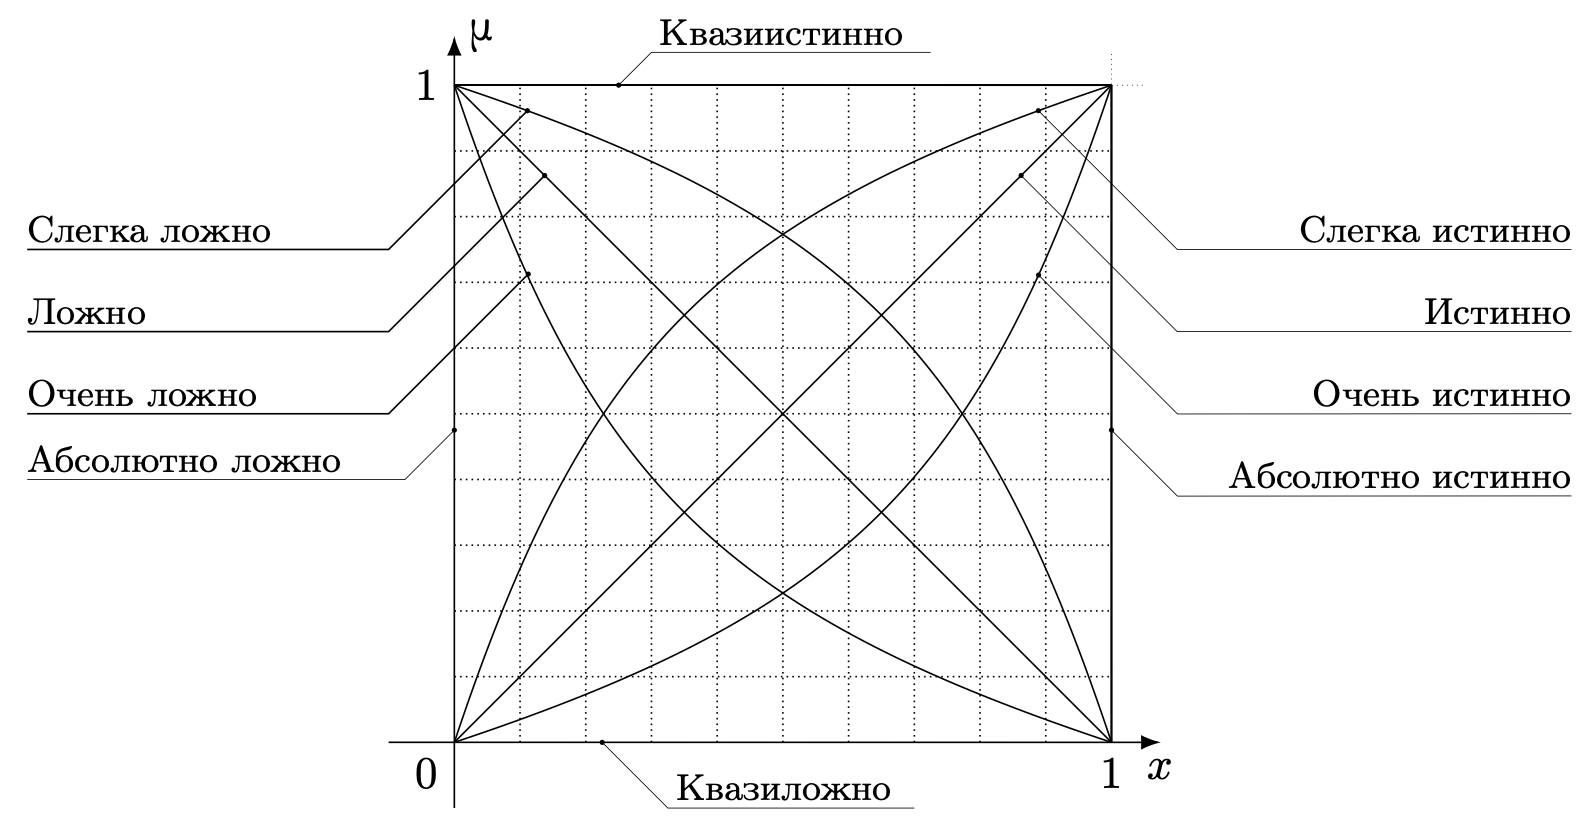
\includegraphics[width=\textwidth]{images/нечеткая истинность.png}
  \caption{Треугольное нечеткое множество и центр тяжести дефаззификации}
  \label{fig:centroid_defuzz}
\end{figure}

\begin{itemize}
  \item $\beta$ — название переменной («истинность»);
  \item $T = \{\text{абсолютно ложно, очень ложно, слегка ложно, ложно,\\
         квазиложно, квазиистинно, истинно, слегка истинно, очень истинно, абсолютно истинно}\}$
        — множество термов;
  \item $X = [0,1]$ — область значений лингвистической переменной;
  \item $G$ — синтаксическая процедура построения составных термов;
  \item $M$ — семантическая процедура, задающая функции принадлежности.
\end{itemize}

\paragraph{Примеры функций принадлежности термов.}
\[
\begin{aligned}
M[\text{«истинно»}](t)&=t,&
M[\text{«слегка истинно»}](t)&=\sqrt{t},\\
M[\text{«очень истинно»}](t)&=t^2,&
M[\text{«абсолютно истинно»}](t)&=
\begin{cases}1,&t=1,\\0,&t<1,\end{cases}\\
M[\text{«ложно»}](t)&=1-t,&
M[\text{«слегка ложно»}](t)&=\sqrt{1-t},\\
M[\text{«очень ложно»}](t)&=(1-t)^2,&
M[\text{«абсолютно ложно»}"](t)&=
\begin{cases}1,&t=0,\\0,&t>0.\end{cases}
\end{aligned}
\]
\begin{figure}[h]
\centering
\begin{tikzpicture}
  \begin{axis}[
    width=0.6\textwidth,
    xlabel={$t$}, ylabel={$\mu$},
    grid=major,
    legend style={at={(1.02,1)},anchor=north west}]
    \addplot {x}; \addlegendentry{истинно}
    \addplot {sqrt(x)}; \addlegendentry{слегка истинно}
    \addplot {x^2}; \addlegendentry{очень истинно}
    \addplot {1-x}; \addlegendentry{ложно}
    \addplot {sqrt(1-x)}; \addlegendentry{слегка ложно}
    \addplot {(1-x)^2}; \addlegendentry{очень ложно}
  \end{axis}
\end{tikzpicture}
\caption{Функции принадлежности лингвистических термов истинности.}
\end{figure}
\paragraph{Лингвистическая интерпретация.}  
\begin{itemize}
  \item «абсолютно истинно», если $\mu_{\CP(A,A')}(t)=1$ на всём диапазоне;
  \item «квазиистинно», если функция близка к 1 на широком промежутке уровней;
  \item «квазиложно», если функция близка к 0 на большинстве уровней;
  \item «абсолютно ложно», если не совпадает ни в одной точке.
\end{itemize}

\paragraph{Дополнительные замечания.}
\begin{itemize}
  \item Методы оценки степени истинности можно расширить на интуитивно-нечёткие множества и другие обобщения.
  \item Для сложных систем часто применяют численные методы приближённого вычисления $\mu_{\CP}(t)$ на дискретной сетке.
  \item Сравнение различных t-норм и импликаций позволяет настраивать «строгость» выводов в нечётких системах.
\end{itemize}
% \subsubsection{Нечёткое значение истинности}
%
% \paragraph{1. Определение и мотивация}
% Числовое значение истинности
% \(\tau_{A/A'}\in[0,1]\)
% задаётся как:
% \begin{equation}
%   \tau_{A/A'}
%   = \sup_{x\in X}\min\{\mu_A(x),\,\mu_{A'}(x)\}.
%   \label{eq:tau_def3b}
% \end{equation}
% Оно отражает максимальную степень одновременного
% "принадлежания" $x$ множествам $A$ и $A'$.
%
% \paragraph{2. Подробное доказательство свойств}
% \begin{theorem}
% Величина $\tau_{A/A'}$:\
% (1) равна 1 тогда и только тогда, когда
% $\mu_A(x)\le\mu_{A'}(x)$ при всех $x$;\
% (2) равна 0 тогда и только тогда,
% когда $\min\{\mu_A(x),\mu_{A'}(x)\}=0$ для всех $x$;\
% (3) монотонна:
% $A_1\subseteq A_2\implies \tau_{A_1/A'}\le \tau_{A_2/A'}$.
% \end{theorem}
%
% \begin{proof}
% Из определения \eqref{eq:tau_def3b} следует,
% что максимум достигается при $x$, где
% $\min(\mu_A,\mu_{A'})$ максимален. Для (1):
% если $\mu_A(x)\le\mu_{A'}(x)$, то
% $\min(\mu_A,\mu_{A'})=\mu_A$ и
% $\sup_x\mu_A(x)=1$. Обратное — аналогично.
% Для (2): $\min(\mu_A,\mu_{A'})=0$ на всех $x$.
% Монотонность — из неубывания $\mu_{A_1}\le\mu_{A_2}$.
% \end{proof}
%
% \begin{figure}[h!]
%   \centering
%   \begin{tikzpicture}[scale=2.5,>=Stealth]
%     \draw[->] (0,0)--(4,0) node[right]{$x$};
%     \draw[->] (0,0)--(0,2) node[above]{$\mu$};
%     \draw[thick,blue,domain=0:4,samples=100]
%       plot(\x,{exp(-((\x-1.3)^2)/0.8)});
%     \node at (1.3,1.6){\footnotesize $\mu_A(x)$};
%     \draw[thick,red,domain=0:4,samples=100]
%       plot(\x,{exp(-((\x-2.7)^2)/1.1)});
%     \node at (2.7,1.1){\footnotesize $\mu_{A'}(x)$};
%     \fill[gray,opacity=0.4]
%       plot[domain=1.6:2.4] (\x,{min(exp(-((\x-1.3)^2)/0.8),exp(-((\x-2.7)^2)/1.1))})
%       -- (2.4,0) -- (1.6,0) -- cycle;
%     \node at (2.0,0.5){\small перекрытие};
%   \end{tikzpicture}
%   \caption{Увеличенный пример: область перекрытия
%     для численного $\tau_{A/A'}$.}
%   \label{fig:tau_enlarged2}
% \end{figure}
%
% Логика, опирающаяся на концепцию нечеткой истинности, обычно именуется лингвистической. 
% В рамках этого подхода «нечеткая истинность» рассматривается как лингвистическая переменная, задаваемая пятёркой
% \[
% \langle \beta,\, T,\, X,\, G,\, M\rangle,
% \]
% где
% \begin{itemize}
%   \item $\beta$ — название переменной («истинность»);
%   \item $T = \{\text{абсолютно ложно, очень ложно, слегка ложно, ложно,\\
%          квазиложно, квазиистинно, истинно, слегка истинно, очень истинно, абсолютно истинно}\}$
%         — множество термов;
%   \item $X = [0,1]$ — область значений лингвистической переменной;
%   \item $G$ — синтаксическая процедура построения составных термов;
%   \item $M$ — семантическая процедура, задающая функции принадлежности.
% \end{itemize}
% \begin{figure}[h]
%   \centering
%   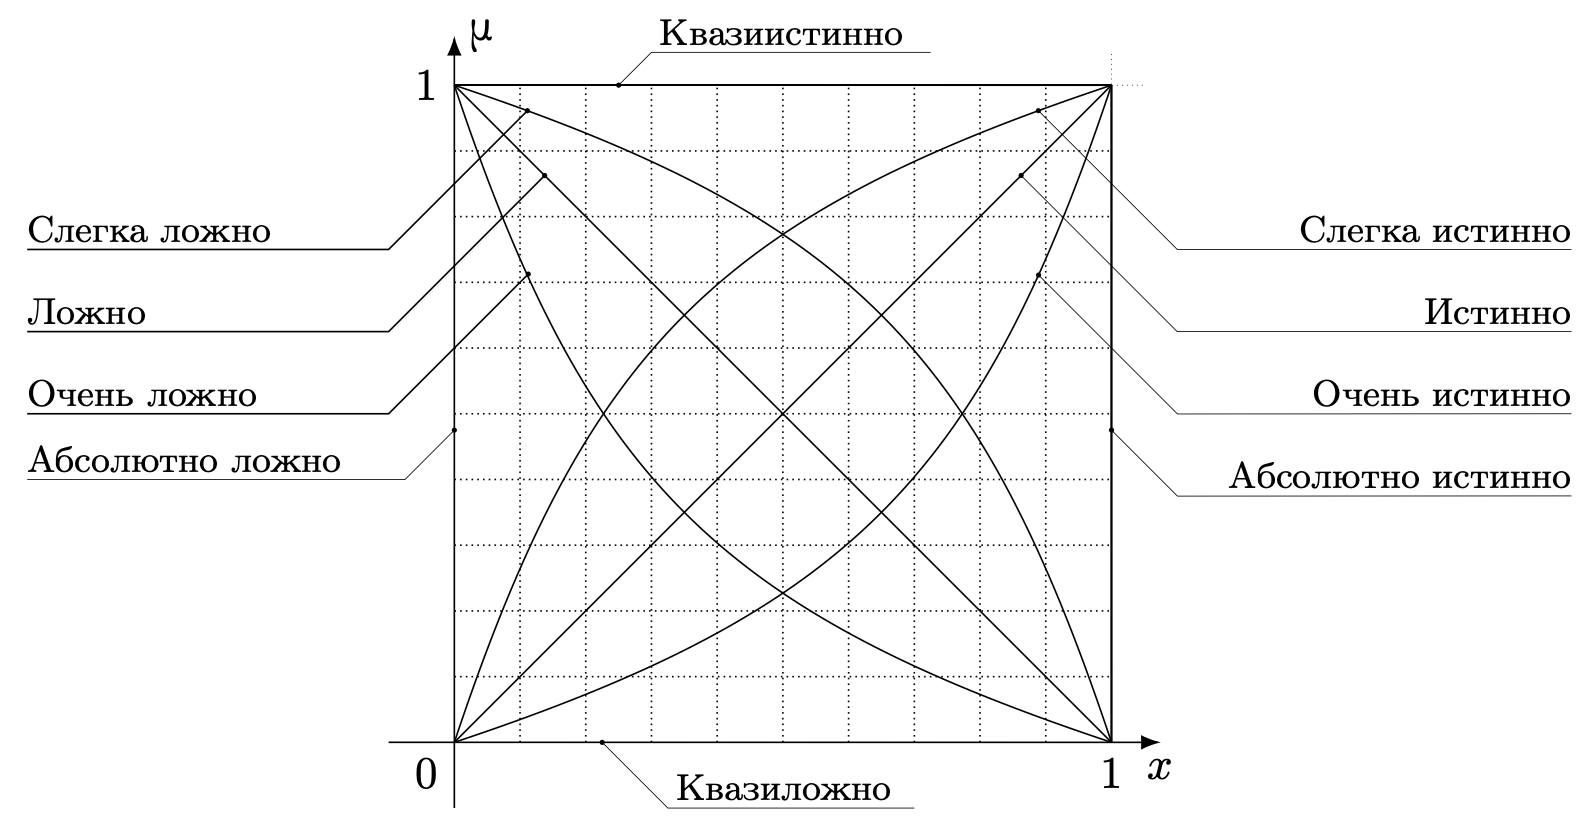
\includegraphics[width=\textwidth]{images/нечеткая истинность.png}
%   \caption{Треугольное нечеткое множество и центр тяжести дефаззификации}
%   \label{fig:centroid_defuzz}
% \end{figure}
% \subsubsection{Методы нечёткого вывода}
% \subsubsection{Нечёткое значение истинности}
% \subsubsection{Нечёткая степень истинности}

% \subsection{Проблемы исходных данных в задачах машинного обучения}
% \subsubsection{Размасштабированность и гетерогенность признаков}
% \subsubsection{Шум, выбросы и пропуски}
% \subsubsection{Несбалансированность классов}
%
% \newpage
%
% \subsection{Обзор инструментальных средств}
% \subsubsection{Выбор языка программирования: Python}
% \subsubsection{Использование GPU: CUDA и PyTorch}
% Лингвистическая логика на основе нечеткой истинности
\subsection{Обзор инструментальных средств}
\label{sec:tools}

\subsubsection{Выбор языка программирования: Python}
\label{sec:tools_python}

Python — язык высокого уровня с лаконичным синтаксисом. Основные преимущества:
\begin{itemize}
  \item Обширная экосистема научных библиотек: \texttt{NumPy}, \texttt{SciPy}, \\ \texttt{Pandas}, \texttt{Matplotlib}
  \item Фреймворки для машинного обучения: \texttt{scikit-learn}, \texttt{TensorFlow}, \\ \texttt{PyTorch}
  \item Быстрое прототипирование в Jupyter;
  \item Большое сообщество и документация.
\end{itemize}

\subsection{Архитектура и оптимизация GPU для обучения нейронных сетей}
\label{ssec:gpu_architecture}

Графические процессоры (GPU) изначально создавались для рендеринга трёхмерной графики, где требовалось одновременно обрабатывать миллионы пикселей. Однако, когда стало ясно, что обучение глубоких нейросетей сводится к повторению единотипных операций над большими массивами чисел, архитектура GPU оказалась почти идеальной. В отличие от CPU с его несколькими быстро работающими ядрами и громоздкой системой предсказания ветвлений, GPU использует сотни или тысячи упрощённых ядер, которые синхронно выполняют одну и ту же инструкцию над разными данными.   

Для понимания того, как они отличаются, достаточно вспомнить, что современные серверные CPU обычно имеют 8–64 полноценных ядра, каждое из которых оснащено суперскалярным исполнителем, многоуровневой кэш-иерархией (L1–L3) и сложной системой предсказания переходов. Такая структура хорошо подходит для разнородных задач — ветвящихся алгоритмов, многозадачности, работы с нерегулярными структурами данных, но она не способна раскрутить более чем десятки параллельных потоков без значительного роста стоимости и энергопотребления.  

GPU же строятся по принципу «массированного параллелизма»: независимые арифметические блоки объединяются в стриминговые мультипроцессоры (Streaming Multiprocessors, SM), а SM, в свою очередь, умножаются до сотен штук на кристалле. Потоки группируются в «warps» (в NVIDIA) или «wavefronts» (в AMD), и все нити в такой группе исполняют одну и ту же инструкцию. Внутри SM есть быстрое локальное хранилище (shared memory) и регистры, что позволяет координировать взаимодействие потоков с минимальной задержкой.  

Память GPU организована в несколько уровней:  
\begin{itemize}  
  \item \emph{Глобальная память (VRAM)} на основе GDDR6 или HBM2/3 обеспечивает пропускную способность до нескольких терабайт в секунду, но обладает заметной латентностью.  
  \item \emph{Кэш уровня L2} объединяет доступы от всех SM и снижает количество обращений к глобальной памяти.  
  \item \emph{Разделяемая память} внутри каждого SM и \emph{регистры} обеспечивают сверхнизкую латентность при обмене данными между соседними тредами.  
\end{itemize}  

Ключевым усовершенствованием последних поколений стало появление тензорных ядер (Tensor Cores), рассчитанных на смешанную точность (обычно FP16/FP32 или BF16). Они позволяют выполнять матричные умножения $4\times4$ или даже $16\times16$ за один такт, что даёт дополнительный прирост производительности в несколько раз при сохранении приемлемой точности сходимости.  

С точки зрения ПО разработчики используют платформы CUDA (NVIDIA) или HIP (AMD), где вся работа разбивается на:  
\begin{itemize}  
  \item \textbf{Запуск кернелов} — небольших программ, которые выполняются на тысячах потоков одновременно.  
  \item \textbf{Асинхронные копирования} (CUDA MemcpyAsync) — перекрытие передачи данных между CPU и GPU с вычислениями, чтобы видеокарта не простаивала.  
  \item \textbf{Стримы и графы задач} — механизм группировки операций для минимизации накладных расходов вызова ядра.  
  \item \textbf{Kernel Fusion} — объединение последовательных операций в единый кернел, позволяющее сократить число обращений к глобальной памяти.  
\end{itemize}  

На практике обучение крупных нейросетей нередко разбивают на две части:  
\begin{enumerate}  
  \item Предобработка, аугментация и загрузка данных (I/O, трансформации) выполняются на CPU, где быстрее работают ветвления и системные вызовы.  
  \item Основной проход (forward/backward) и обновление параметров — на GPU, где тысячи ядер решают одинаковые подзадачи над матрицами и тензорами.  
\end{enumerate}  

Визуализация профилей реальных задач показывает, что современные ускорители типа NVIDIA A100 обеспечивают до 1–1.5 PFLOPS в смешанной точности при потреблении порядка 300 Вт, тогда как эквивалентная нагрузка на серверный CPU (Intel Xeon) даст лишь пару сотен GFLOPS при схожем энергопотреблении. Это объясняет, почему GPU остаются ключевым ресурсом для дата-центров машинного обучения.  

Конечно, у GPU есть и ограничения:  
\begin{itemize}  
  \item \textbf{Ограниченный объём VRAM}. Модели типа GPT-3 XXL могут не помещаться на одной карте, требуя шардирования по нескольким GPU.  
  \item \textbf{Высокая латентность случайных доступов} к памяти усложняет нерегулярные вычисления и динамические графы.  
  \item \textbf{Накладные расходы} на передачу данных по PCIe/NVLink (несколько миллисекунд при больших объёмах).  
  \item \textbf{Сложность отладки} параллельных алгоритмов и профилирования (нужны специальные инструменты: Nsight, rocProfiler).  
\end{itemize}  


\subsubsection{Использование GPU: CUDA и PyTorch}
\label{sec:tools_gpu}

\paragraph{Модель программирования CUDA}
Программист описывает kernel-функции, которые запускаются параллельно. Пример сложения двух векторов:

\begin{lstlisting}[language=C,caption={CUDA: сложение векторов},label={lst:cuda_vecadd}]
__global__ void vecAdd(const float *A, const float *B, float *C, int N) {
    int i = blockIdx.x * blockDim.x + threadIdx.x;
    if (i < N) {
        C[i] = A[i] + B[i];
    }
}

float *d_A, *d_B, *d_C;
cudaMalloc(&d_A, N * sizeof(float));
cudaMalloc(&d_B, N * sizeof(float));
cudaMalloc(&d_C, N * sizeof(float));
cudaMemcpy(d_A, h_A, N * sizeof(float), cudaMemcpyHostToDevice);

int blockSize = 256;
int gridSize  = (N + blockSize - 1) / blockSize;
vecAdd<<<gridSize, blockSize>>>(d_A, d_B, d_C, N);

cudaMemcpy(h_C, d_C, N * sizeof(float), cudaMemcpyDeviceToHost);
\end{lstlisting}

\paragraph{Оптимизации для CUDA}
\begin{itemize}
  \item Coalesced memory access: чтение подряд идущих адресов одним warp\;
  \item Shared memory для уменьшения обращений к глобальной памяти\;
  \item Асинхронное копирование и стримы (\texttt{cudaMemcpyAsync}, \texttt{cudaStream}) для перекрытия вычислений и передачи данных.
\end{itemize}

\paragraph{PyTorch и GPU}
PyTorch позволяет легко переносить тензоры на устройство и выполнять вычисления:

\begin{lstlisting}[language=Python,caption={PyTorch: базовые операции на GPU},label={lst:torch_gpu}]
import torch

t = torch.randn(1024, 1024, device='cuda')

y = torch.mm(t, t)

x = torch.tensor([1., 2., 3.], device='cuda', requires_grad=True)
y = x.pow(2).sum()
y.backward()
print(x.grad)  # tensor([2., 4., 6.], device='cuda:0')
\end{lstlisting}

\paragraph{Сравнение библиотек}
\textbf{TensorFlow} (статический граф):
\begin{lstlisting}[language=Python,caption={TensorFlow: определение и запуск функции},label={lst:tf}]
import tensorflow as tf

@tf.function
def fwd(x):
    return tf.matmul(x, x)

x = tf.random.normal((1024, 1024))
y = fwd(x)
\end{lstlisting}

\textbf{JAX} (JIT и векторизация):
\begin{lstlisting}[language=Python,caption={JAX: JIT-компиляция и градиент},label={lst:jax}]
import jax.numpy as jnp
from jax import jit, grad

@jit
def f(x):
    return jnp.dot(x, x)

res = f(jnp.ones((1024, 1024)))
g = grad(lambda m: jnp.sum(m**2))(jnp.ones((3,)))
\end{lstlisting}

\textbf{MXNet} (Gluon API):
\begin{lstlisting}[language=Python,caption={MXNet: dot-операция на GPU},label={lst:mxnet}]
from mxnet import nd, gpu

x = nd.random.normal(shape=(1024,1024), ctx=gpu())
w = nd.random.normal(shape=(1024,1024), ctx=gpu())
y = nd.dot(x, w)
\end{lstlisting}

PyTorch выделяется динамическим графом и удобством отладки, TensorFlow — оптимизацией статических моделей, JAX — простотой JIT и векторизации, MXNet — гибкостью Gluon API.

\subsection{Методы предварительной обработки и улучшения данных}

В современных задачах машинного обучения и анализа данных качество результатов во многом зависит от корректности и информативности исходных признаков. Процесс \emph{предварительной обработки} (preprocessing) включает в себя целый набор операций, направленных на приведение данных к удобному для моделей виду, снижение шумов и балансировку выборки. Ниже приведены три ключевых группы методов: масштабирование, синтетическое дополнение редких классов и работа с выбросами. Для каждой группы описаны цели, основные подходы, преимущества и ограничения, а также приведены примеры формул и кода на Python.

% ----------------------------------------
\subsubsection{Масштабирование}
\label{sec:scaling}

\paragraph{Зачем нужно масштабирование?}  
Многие алгоритмы (например, методы на основе евклидова расстояния или градиентного спуска) чувствительны к масштабу признаков. Если один признак принимает значения от 0 до 1, а другой — от \(10^3\) до \(10^6\), модель будет «смотреть» в первую очередь на крупномасштабный признак. Кроме того, плохая масштабировка может замедлять сходимость оптимизации.

\paragraph{Основные методы}
\begin{itemize}
  \item \textbf{Min–Max нормализация:}  
    \[
      x' = \frac{x - x_{\min}}{x_{\max} - x_{\min}},
      \quad x'\in[0,1].
    \]
    \emph{Плюсы:} сохраняет форму распределения, легко интерпретировать.  
    \emph{Минусы:} чувствительна к выбросам, требует знания глобальных минимумов и максимумов.
    
  \item \textbf{Z-преобразование (Standardization):}  
    \[
      x' = \frac{x - \mu}{\sigma},
      \quad \mu = \frac{1}{n}\sum_i x_i,\;
      \sigma = \sqrt{\frac{1}{n}\sum_i (x_i - \mu)^2}.
    \]
    \emph{Плюсы:} приводит данные к нулевому среднему и единичному стандартному отклонению, устойчиво при небольших выбросах.  
    \emph{Минусы:} всё ещё может страдать от сильных выбросов.
    
  \item \textbf{Десятичное масштабирование:}  
    \[
      x' = \frac{x}{10^j},\quad
      j = \left\lceil \log_{10}\bigl(\max_i |x_i|\bigr)\right\rceil.
    \]
    \emph{Плюсы:} просто реализуется, гарантирует \(|x'|<1\).  
    \emph{Минусы:} не выравнивает распределение, работает только с десятичной шкалой.
    
  \item \textbf{Робастное масштабирование:}  
    \[
      x' = \frac{x - \mathrm{median}(x)}{\mathrm{IQR}(x)},
      \quad \mathrm{IQR} = Q_3 - Q_1.
    \]
    \emph{Плюсы:} устойчиво к выбросам.  
    \emph{Минусы:} требует расчёта квартилей, менее распространено.
\end{itemize}

\paragraph{Снижение размерности как частный случай}  
Иногда под «масштабированием» понимают удаление избыточных признаков.  
\begin{itemize}
  \item \emph{PCA} (метод главных компонент): решается собственная задача для ковариационной матрицы и берутся \(k\) ведущих компонент:
    \[
      X' = XW,\quad W = [v_1,\dots,v_k],\quad \Sigma v_i = \lambda_i v_i.
    \]
  \item \emph{LDA} (линейный дискриминантный анализ): максимизация отношения межклассовой и внутриклассовой дисперсии.
  \item Нелинейные методы \emph{t-SNE}, \emph{UMAP} — для визуализации в 2–3D.
\end{itemize}

\paragraph{Пример на Python}
\begin{lstlisting}[language=Python]
from sklearn.preprocessing import MinMaxScaler, StandardScaler
from sklearn.decomposition import PCA

mm = MinMaxScaler(feature_range=(0,1))
X_mm = mm.fit_transform(X)

std = StandardScaler()
X_std = std.fit_transform(X)

pca = PCA(n_components=2, random_state=42)
X_pca = pca.fit_transform(X_std)
\end{lstlisting}

% ----------------------------------------
\subsubsection{Синтетическое дополнение редких классов}
\label{sec:oversampling}

\paragraph{Почему важно дополнять редкие классы?}  
В случае сильного дисбаланса модель может «игнорировать» малочисленные классы, отказываться им уделять внимание и выдавать предсказания лишь для большинства. Синтетическое дополнение (oversampling) помогает сгладить этот эффект, повысить чувствительность к редким событиям и улучшить общую сбалансированность.

\paragraph{Методы синтеза}
\begin{enumerate}
  \item \textbf{SMOTE} (Synthetic Minority Over-sampling Technique):  
    Для каждой точки \(x_i\) класса-минорити выбирается один из \(k\) ближайших соседей \(x_{\rm nn}\) и синтезируется:
    \[
      x_{\rm new} = x_i + \delta\,(x_{\rm nn} - x_i),\quad \delta\in[0,1].
    \]
  \item \textbf{Borderline-SMOTE}:  
    Генерация новых примеров только в «пограничных» зонах, где редкий класс пересекается с мажорити.
  \item \textbf{ADASYN}:  
    Учитывает плотность объектов, создаёт больше синтетических точек там, где редкий класс особенно редок.
  \item \textbf{GAN-базированные методы}:  
    Обучают генератор/дискриминатор для создания правдоподобных новых образцов.
\end{enumerate}

\paragraph{Плюсы и минусы}
\begin{itemize}
  \item \emph{Плюсы:}  
    \begin{itemize}
      \item Сглаживает дисбаланс без потери информации.  
      \item Увеличивает объём обучающей выборки, что может улучшить регуляризацию.
    \end{itemize}
  \item \emph{Минусы:}  
    \begin{itemize}
      \item Риск переобучения на синтетических данных.  
      \item При сложном многомерном распределении могут появиться «ненатуральные» точки.
    \end{itemize}
\end{itemize}

\paragraph{Пример на Python}
\begin{lstlisting}[language=Python]
from imblearn.over_sampling import SMOTE

smote = SMOTE(sampling_strategy='minority', k_neighbors=5, random_state=42)
X_res, y_res = smote.fit_resample(X, y)
\end{lstlisting}

% ----------------------------------------
\subsubsection{Обнаружение и устранение выбросов}
\label{sec:outliers}

\paragraph{Зачем искать выбросы?}  
Выбросы могут искажать оценки параметров (среднее, дисперсию), влиять на обучение моделей и ухудшать обобщающую способность. При этом не все «экстремальные» значения — ошибки: порой это важные редкие события.

\paragraph{Методы обнаружения}
\begin{itemize}
  \item \textbf{Статистические критерии:}
    \begin{itemize}
      \item Z-score: 
        $|z_i| > \tau$, где обычно $\tau\approx3$.
      \item IQR-критерий: 
        $x < Q_1 - 1.5\,\mathrm{IQR}$ или $x > Q_3 + 1.5\,\mathrm{IQR}$.
    \end{itemize}

  \item \textbf{Алгоритмические методы:}
    \begin{itemize}
      \item Isolation Forest: строит деревья, в которых «аномалии» изолируются быстрее.
      \item Local Outlier Factor: сравнивает плотность вокруг точки с плотностью у соседей.
      \item One-Class SVM: обучается только на «нормальных» данных и выявляет выбросы.
    \end{itemize}
\end{itemize}

\paragraph{Стратегии устранения}
\begin{itemize}
  \item \emph{Удаление:} простое отбрасывание аномальных строк.
  \item \emph{Замена:} подстановка медианы, моды или крайних значений.
  \item \emph{Капирование (capping):} обрезание выходящих за пределы значений до выбранных порогов.
\end{itemize}

\begin{table}[h]
\centering
\caption{Плюсы и минусы}
\label{tab:pros_cons}
\begin{tabularx}{\textwidth}{@{}>{\raggedright\arraybackslash}X>{\raggedright\arraybackslash}X@{}}
\toprule
\textbf{Плюсы} & \textbf{Минусы} \\
\midrule
Повышает надёжность статистических оценок. & Можно случайно удалить важные редкие события. \\
\addlinespace[0.5em]
Облегчает обучение моделей, снижает риск переобучения на шуме. & Сложно задать универсальные пороги для разных признаков. \\
\bottomrule
\end{tabularx}
\end{table}

\paragraph{Пример на Python}
\begin{lstlisting}[language=Python]
import numpy as np
from sklearn.ensemble import IsolationForest

z_scores = (X - X.mean(axis=0)) / X.std(axis=0)
mask = np.all(np.abs(z_scores) < 3, axis=1)
X_clean_z = X[mask]

iso = IsolationForest(contamination=0.05, random_state=0)
labels = iso.fit_predict(X)
X_clean_if = X[labels == 1]
\end{lstlisting}

% ----------------------------------------
% Конец раздела
% ----------------------------------------
% \subsection{Методы предварительной обработки и улучшения данных}
% \subsubsection{Масштабировани}
% \subsubsection{Синтетическое дополнение редких классов (SMOTE)}
% \subsubsection{Обнаружение и устранение выбросов}
%
\subsection{Инструменты и методы оптимизации гиперпараметров}
\label{sec:hyperparameter-optimization}

Под гиперпараметрами понимаются конфигурационные параметры модели или алгоритма, устанавливаемые до начала процесса обучения или инициализации и не обновляемые в процессе градиентного спуска или другого метода оптимизации. К классическим примерам относятся скорость обучения, глубина дерева решений, число скрытых слоёв нейросети и параметры регуляризации. Более того, в гибридных системах нейронно-нечеткой логики гиперпараметрами могут быть весовые коэффициенты правил нечеткого вывода, параметры функций принадлежности и пороги активации. Корректный подбор гиперпараметров напрямую влияет на качество работы модели, скорость её сходимости, устойчивость к переобучению и способность адаптироваться к сложным неопределённым условиям.

\subsubsection{Классические методы}

\paragraph{Перебор по сетке (Grid Search)}  
Пусть для каждого из \(k\) гиперпараметров задано дискретное множество \(P_i\), \(|P_i|=n_i\). Тогда полный перебор предполагает проверку всех комбинаций:
\begin{equation}
\mathcal{P} \;=\; P_1 \times P_2 \times \cdots \times P_k,
\qquad
|\mathcal{P}| \;=\; \prod_{i=1}^k n_i.
\label{eq:grid-search-size}
\end{equation}
\textbf{Плюсы:} простота реализации, гарантированное покрытие решётки.  
\textbf{Минусы:} экспоненциальный рост числа испытаний при увеличении \(k\) и \(n_i\).

\paragraph{Случайный поиск (Random Search)}  
При ограниченном бюджете \(N\) испытаний точки выбираются в гиперпространстве равномерно:
\begin{equation}
p_i^{(j)} \;\sim\; \mathcal{U}(a_i, b_i),
\quad j = 1,\dots,N.
\label{eq:random-search}
\end{equation}
\citet{bergstra2012random} показали, что при фиксированном \(N\) Random Search часто эффективнее Grid Search, так как распределяет усилия по более важным измерениям.

\subsubsection{Байесовская оптимизация}

Методы байесовской оптимизации строят суррогатную модель целевой функции
\(
f\colon \mathcal{X}\to\mathbb{R}
\)
на основе предыдущих наблюдений \(\mathcal{D}=\{(x_i, f(x_i))\}\) и используют функцию приобретения \(\alpha(x)\) для выбора следующей точки:
\begin{equation}
x_{n+1} = \arg\max_{x\in\mathcal{X}} \alpha\bigl(x;\,p(f\mid\mathcal{D})\bigr).
\label{eq:bayes-opt}
\end{equation}

\paragraph{Gaussian Process (GP)}  
Суррогатная модель задаётся процессом:
\begin{equation}
f(x)\sim\mathcal{GP}\bigl(m(x),\,k(x,x')\bigr),
\label{eq:gp-prior}
\end{equation}
где \(m(x)\) — функция среднего, \(k(x,x')\) — ковариационное ядро. По данным \(\mathcal{D}\) получают предсказание \(\mu_n(x)\) и неопределённость \(\sigma_n(x)\).

\paragraph{Функции приобретения}  
\begin{align}
\mathrm{EI}(x)
&= (f_{\min}-\mu_n(x))\,\Phi\bigl(Z\bigr)
+ \sigma_n(x)\,\phi\bigl(Z\bigr),
\quad Z = \frac{f_{\min}-\mu_n(x)}{\sigma_n(x)},
\label{eq:expected-improvement}\\
\mathrm{PI}(x)
&= \Phi\!\Bigl(\frac{f_{\min}-\mu_n(x)}{\sigma_n(x)}\Bigr),
\label{eq:probability-improvement}\\
\mathrm{UCB}(x)
&= \mu_n(x) - \kappa\,\sigma_n(x).
\label{eq:upper-conf-bound}
\end{align}

\subsubsection{Адаптивное распределение ресурсов}

\paragraph{Successive Halving}  
Все \(n\) конфигураций обучаются на малом бюджете \(r\), затем отбираются лучшие \(n/\eta\) и их обучают с бюджетом \(\eta r\), и так далее.

\paragraph{Hyperband / ASHA}  
Комбинирует Successive Halving с несколькими начальными бюджетами \(r_1, r_2, \dots, r_s\), что позволяет балансировать между шириной и глубиной поиска.

\subsubsection{Современные фреймворки}

\begin{itemize}
  \item \textbf{Optuna}. Основан на TPE (Tree-structured Parzen Estimator).
  \item \textbf{Hyperopt}. Реализует TPE и Random Search, конфигурируется через Python-словари.
  \item \textbf{Scikit-Optimize (skopt)}. Предоставляет \texttt{gp\_minimize},  \\
    \texttt{forest\_minimize}, \texttt{gbrt\_minimize}.
  \item \textbf{Ray Tune}. Распределённая оптимизация с поддержкой HyperOpt, BayesOpt, HyperBand.
  \item \textbf{SMAC}. Bayesian Optimization на основе Random Forest.
\end{itemize}

\subsubsection{Пример использования Optuna}

\begin{lstlisting}[language=Python]
import optuna

def objective(trial):
    lr = trial.suggest_loguniform('learning_rate', 1e-5, 1e-1)
    n_estimators = trial.suggest_int('n_estimators', 50, 500)
    score = train_and_evaluate(lr, n_estimators)
    return score

study = optuna.create_study(direction='minimize')
study.optimize(objective, n_trials=50)
\end{lstlisting}

\section{Программная реализация}

\subsection{Предобработка данных}

Прежде чем приступить к построению и обучению любой интеллектуальной системы — будь то нейронная сеть, нечеткая система или гибридный метод — критически важно убедиться в качестве и корректности входных данных. Современные алгоритмы машинного обучения крайне чувствительны к шуму, выбросам, разным масштабам признаков и пропускам, поэтому этап предобработки часто определяет успешность всей работы.

В качестве демонстрационного примера я использовал классический набор данных Iris\footnote{Fisher R.A. (1936). \emph{The use of multiple measurements in taxonomic problems}. Annals of Eugenics, 7(2):179–188.}. Этот набор содержит 150 образцов ирисов трёх видов (\emph{Iris setosa}, \emph{Versicolor}, \emph{Virginica}), описанных четырьмя числовыми признаками:
\begin{itemize}
  \item длина чашелистика (sepal length), см;
  \item ширина чашелистика (sepal width), см;
  \item длина лепестка (petal length), см;
  \item ширина лепестка (petal width), см.
\end{itemize}
Каждому образцу сопоставлен целевой класс — один из трёх видов ириса.

\medskip
\noindent\textbf{Основные этапы предобработки данных:}
\begin{enumerate}
  \item \textbf{Первичный анализ}  
    \begin{itemize}
      \item Проверка отсутствующих значений и аномалий.
      \item Вычисление базовых статистик (среднее, стандартное отклонение, квартили).
      \item Визуализация распределений (гистограммы) и парных зависимостей (scatter–matrix).
    \end{itemize}
  \item \textbf{Выявление и удаление выбросов}  
    С помощью межквартильного метода и визуальных средств (ящика с усами) отмечаются экстремальные значения, которые могут искажать обучение.
  \item \textbf{Нормализация и масштабирование}  
    Для равномерного вклада всех признаков используется стандартизация (z-score) или min–max нормализация:
    \[
      x' = \frac{x - \mu}{\sigma},\quad
      x'' = \frac{x - x_{\min}}{x_{\max}-x_{\min}}.
    \]
  \item \textbf{Разбиение на обучающую и тестовую выборки}  
    Обычно данные делятся в соотношении 70\%–30\% или 80\%–20\%, с последующим стратифицированным отбором образцов, чтобы сохранить пропорции классов.
\end{enumerate}

\subsection{Инструменты анализа}

Для качественной предобработки и первичной оценки данных используются следующие ключевые приёмы визуализации:

\begin{description}
  \item[Гистограмма (Histogram)]  
    \hfill 
    \begin{itemize}
      \item \textbf{Назначение:} 
        
        оценить форму распределения одного числового признака, выявить асимметрию, мультимодальность и выбросы.
      \item \textbf{Как читать:} 
        
        по горизонтали — интервалы значений (бины), по вертикали — количество образцов.  
      \item \textbf{Рекомендации:}  
        \begin{itemize}
          \item Подберите число бинов так, чтобы не терялось основное «полотно» распределения, но и не было слишком «рвано».  
          \item Обратите внимание на пики — возможные подгруппы данных.  
          \item Узкие «хвосты» помогут заметить редкие выбросы.
        \end{itemize} 
    \end{itemize}

  \item[Boxplot–диаграмма (Box–Whisker)]  
    \hfill
    \begin{itemize}
      \item \textbf{Назначение:} 
        
        сравнить распределения одного признака между группами (видами iris), одновременно увидеть медиану, квартильные границы и выбросы.
      \item \textbf{Как читать:}  
        \begin{itemize}
          \item Ящик (box) — межквартильный интервал (Q1–Q3), линия внутри — медиана.  
          \item Усы (whiskers) — выборочные границы (обычно Q1−-1.5 \cdot IQR, Q3+1.5 \cdot IQR).  
          \item Точки за усами — выбросы.
        \end{itemize}
      \item \textbf{Рекомендации:}  
        \begin{itemize}
          \item Сравнивайте положения медиан для разных групп.  
          \item Используйте одну палитру для согласованности.  
          \item При разметке терминов в нечеткой системе берите Q1, Q2, Q3 как опорные точки.
        \end{itemize}
    \end{itemize}

  \item[Матрица рассеяния (Scatter–matrix)]  
    \hfill
    \begin{itemize}
      \item \textbf{Назначение:} 
        
        одновременно визуализировать попарные зависимости и распределения всех признаков.
      \item \textbf{Как читать:}  
        \begin{itemize}
          \item Диагональные ячейки — гистограммы каждого признака.  
          \item Вне диагонали — точечные диаграммы (scatter plots) для пары признаков.
        \end{itemize}
      \item \textbf{Рекомендации:}  
        \begin{itemize}
          \item Ищите пары с минимальным перекрытием классов — эти сочетания наиболее информативны для классификатора.  
          \item Линейная или кластераная структура подскажет, что выбирать в качестве antecedent–признаков.
        \end{itemize}
    \end{itemize}

  \item[K–Means кластеризация (Cluster Plot)]  
    \hfill
    \begin{itemize}
      \item \textbf{Назначение:} быстро оценить естественную группировку данных в выбранном признаковом пространстве.
      \item \textbf{Как читать:}  
        \begin{itemize}
          \item Точки раскрашены по присвоенному кластеру.  
          \item Центроиды отображаются метками (крестиками).  
          \item Легенда и подписи кластеров помогают связать группы с реальными классами.
        \end{itemize}
      \item \textbf{Рекомендации:}  
        \begin{itemize}
          \item Используйте кластер-плот для предпосева числа терминов в нечеткой системе.  
          \item Оценивайте степень «смешивания» точек разных классов внутри одного кластера.  
          \item Корректируйте число кластеров ($k$) и наблюдайте устойчивость центроидов.
        \end{itemize}
    \end{itemize}
\end{description}

\subsection{Анализ исходных данных (Iris Dataset)}


Прежде чем приступать к построению нечеткой сети, необходимо тщательно изучить и подготовить исходный датасет. В качестве демонстрационного примера мы используем классический набор \emph{Iris} (150 образцов, 4 числовых признака, 3 класса).

\subsubsection{Статистическое описание}
\begin{table}[H]
  \centering
  \caption{Базовые статистические характеристики признаков Iris Dataset.}
  \begin{tabular}{lrrrr}
    \toprule
    Признак & Среднее & СКО & Мин. & Макс. \\
    \midrule
    sepal length (cm) & 5.84 & 0.83 & 4.30 & 7.90 \\
    sepal width  (cm) & 3.06 & 0.44 & 2.00 & 4.40 \\
    petal length (cm) & 3.76 & 1.77 & 1.00 & 6.90 \\
    petal width  (cm) & 1.20 & 0.76 & 0.10 & 2.50 \\
    \bottomrule
  \end{tabular}
  \label{tab:iris_stats}
\end{table}

\subsubsection{Распределение признаков}

На рис.~\ref{fig:iris_histos} представлены гистограммы всех четырёх признаков, построенные с цветовой палитрой.
\begin{figure}[H]
  \centering
  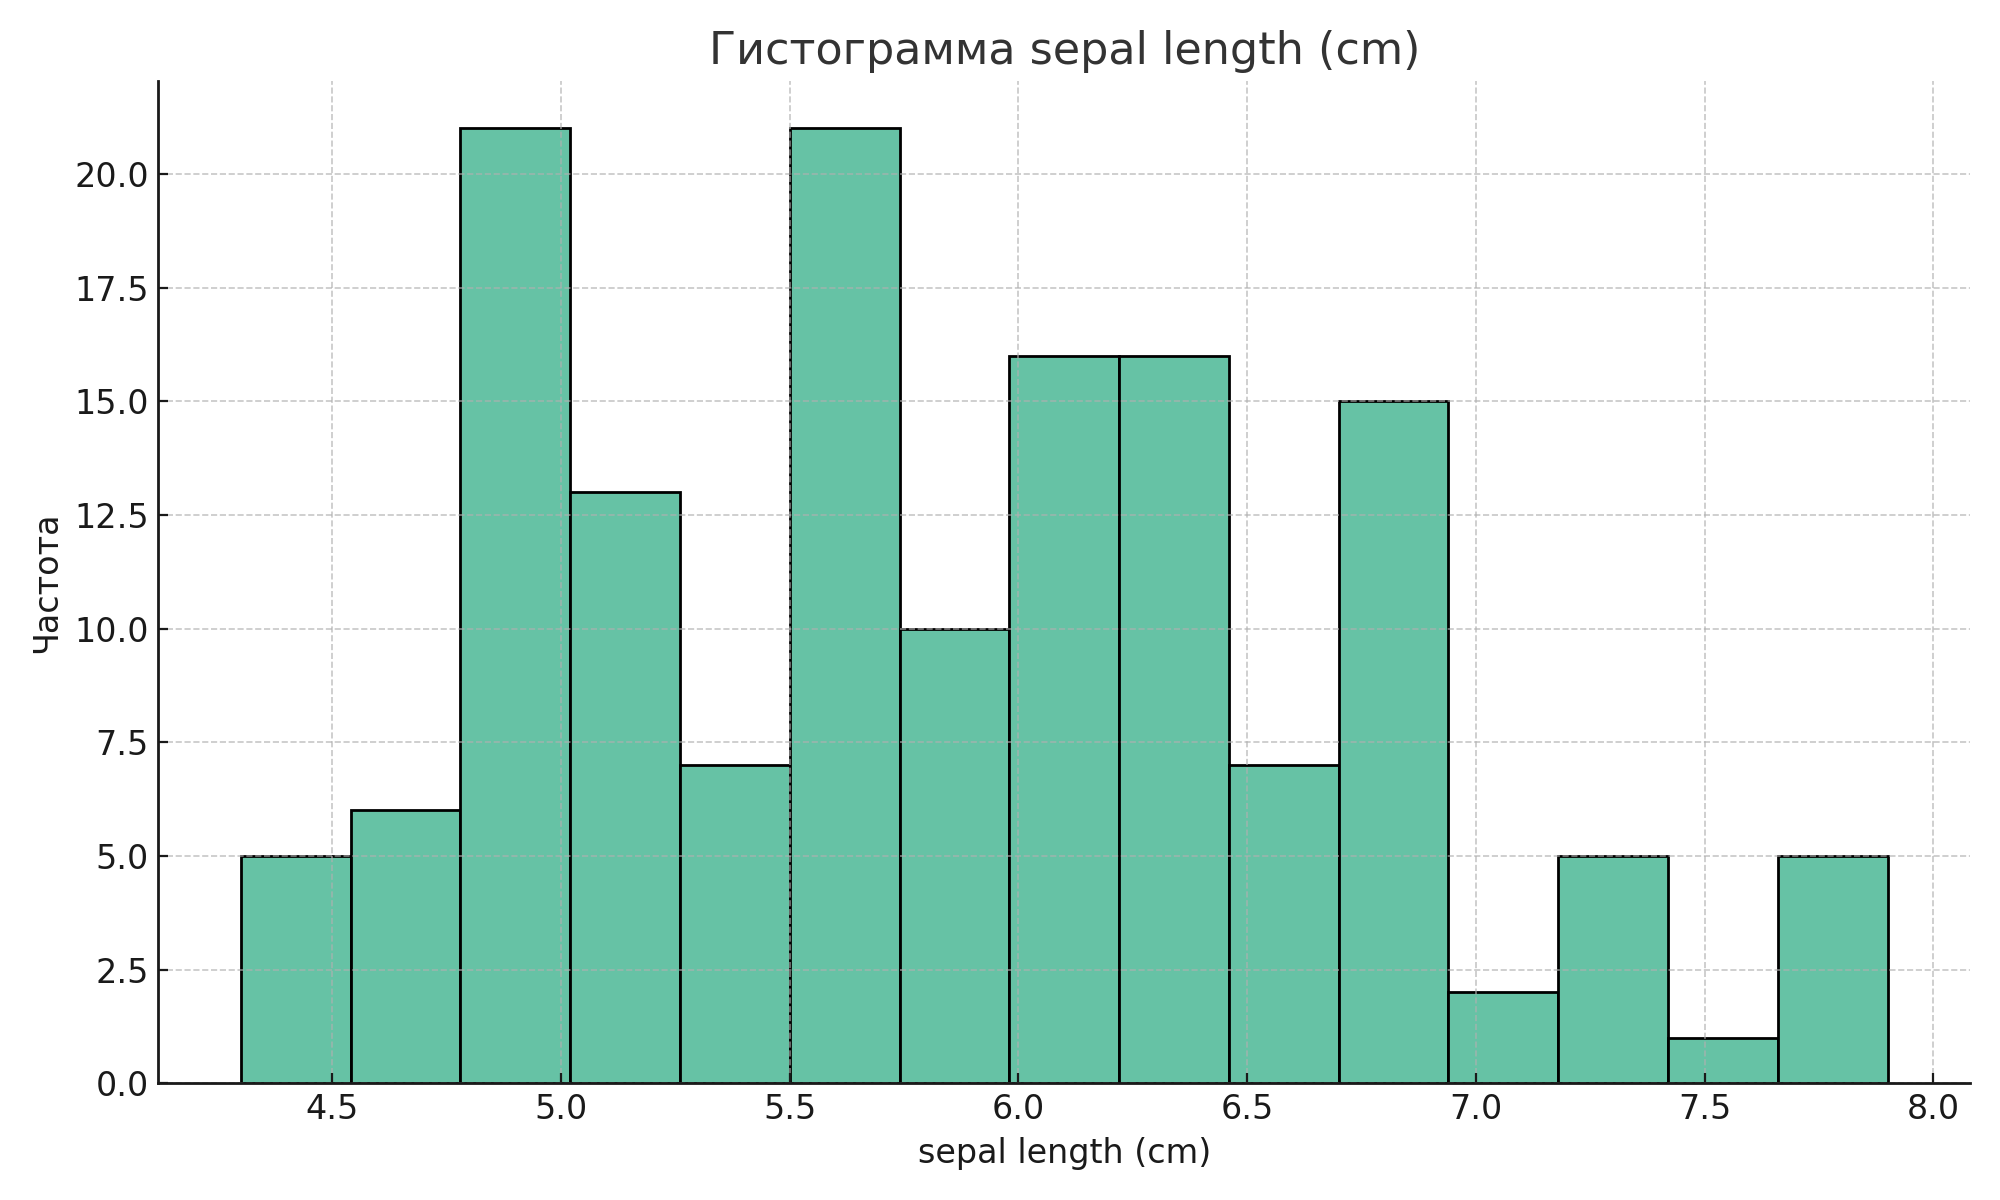
\includegraphics[width=0.8\textwidth]{images/histo_sepal_length_cm_cb2.png}\\[6pt]
  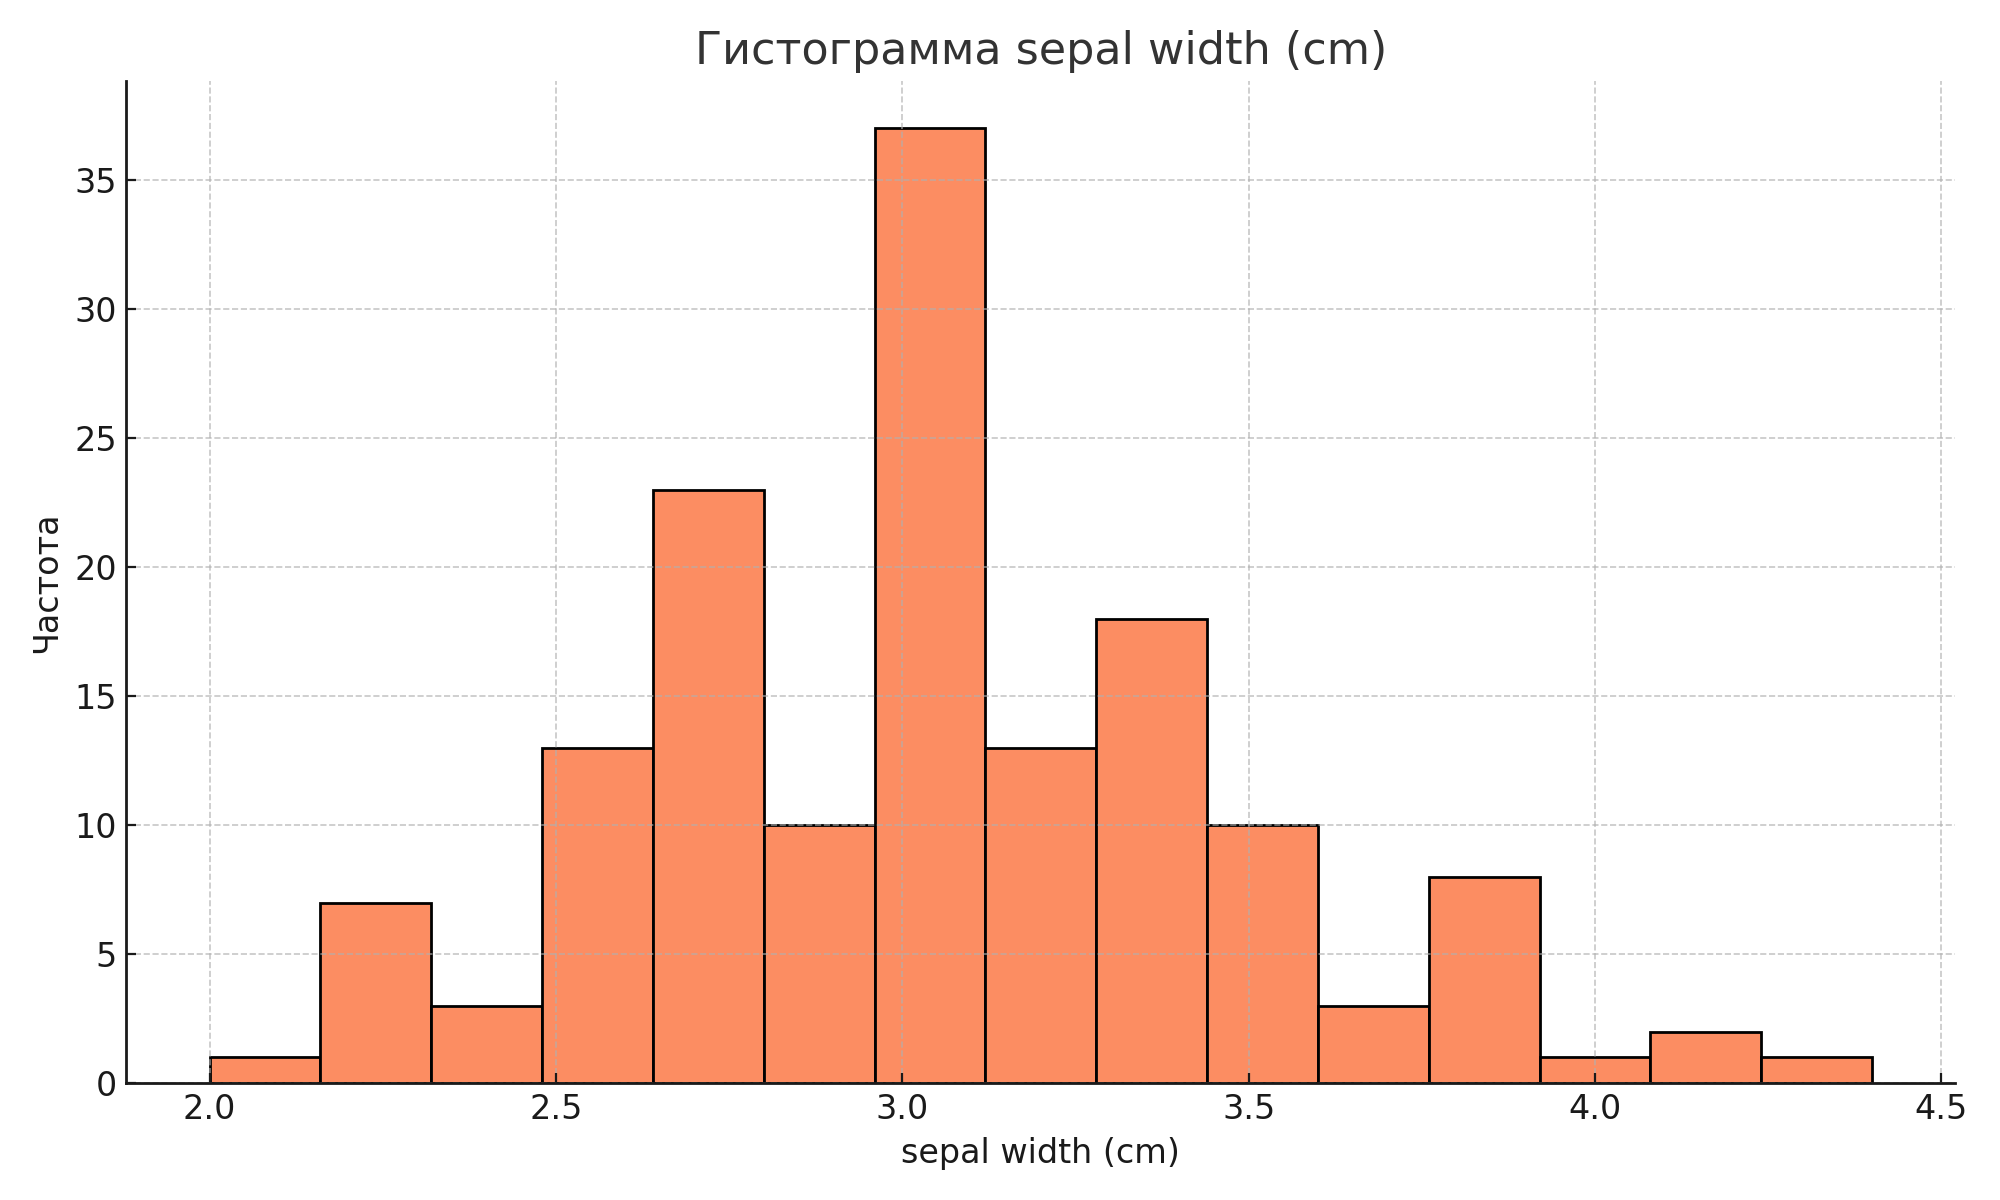
\includegraphics[width=0.8\textwidth]{images/histo_sepal_width_cm_cb2.png}
  \caption{Гистограммы распределений признаков Iris Dataset.}
  \label{fig:iris_histos}
\end{figure}

\begin{figure}[H]\ContinuedFloat
  \centering
  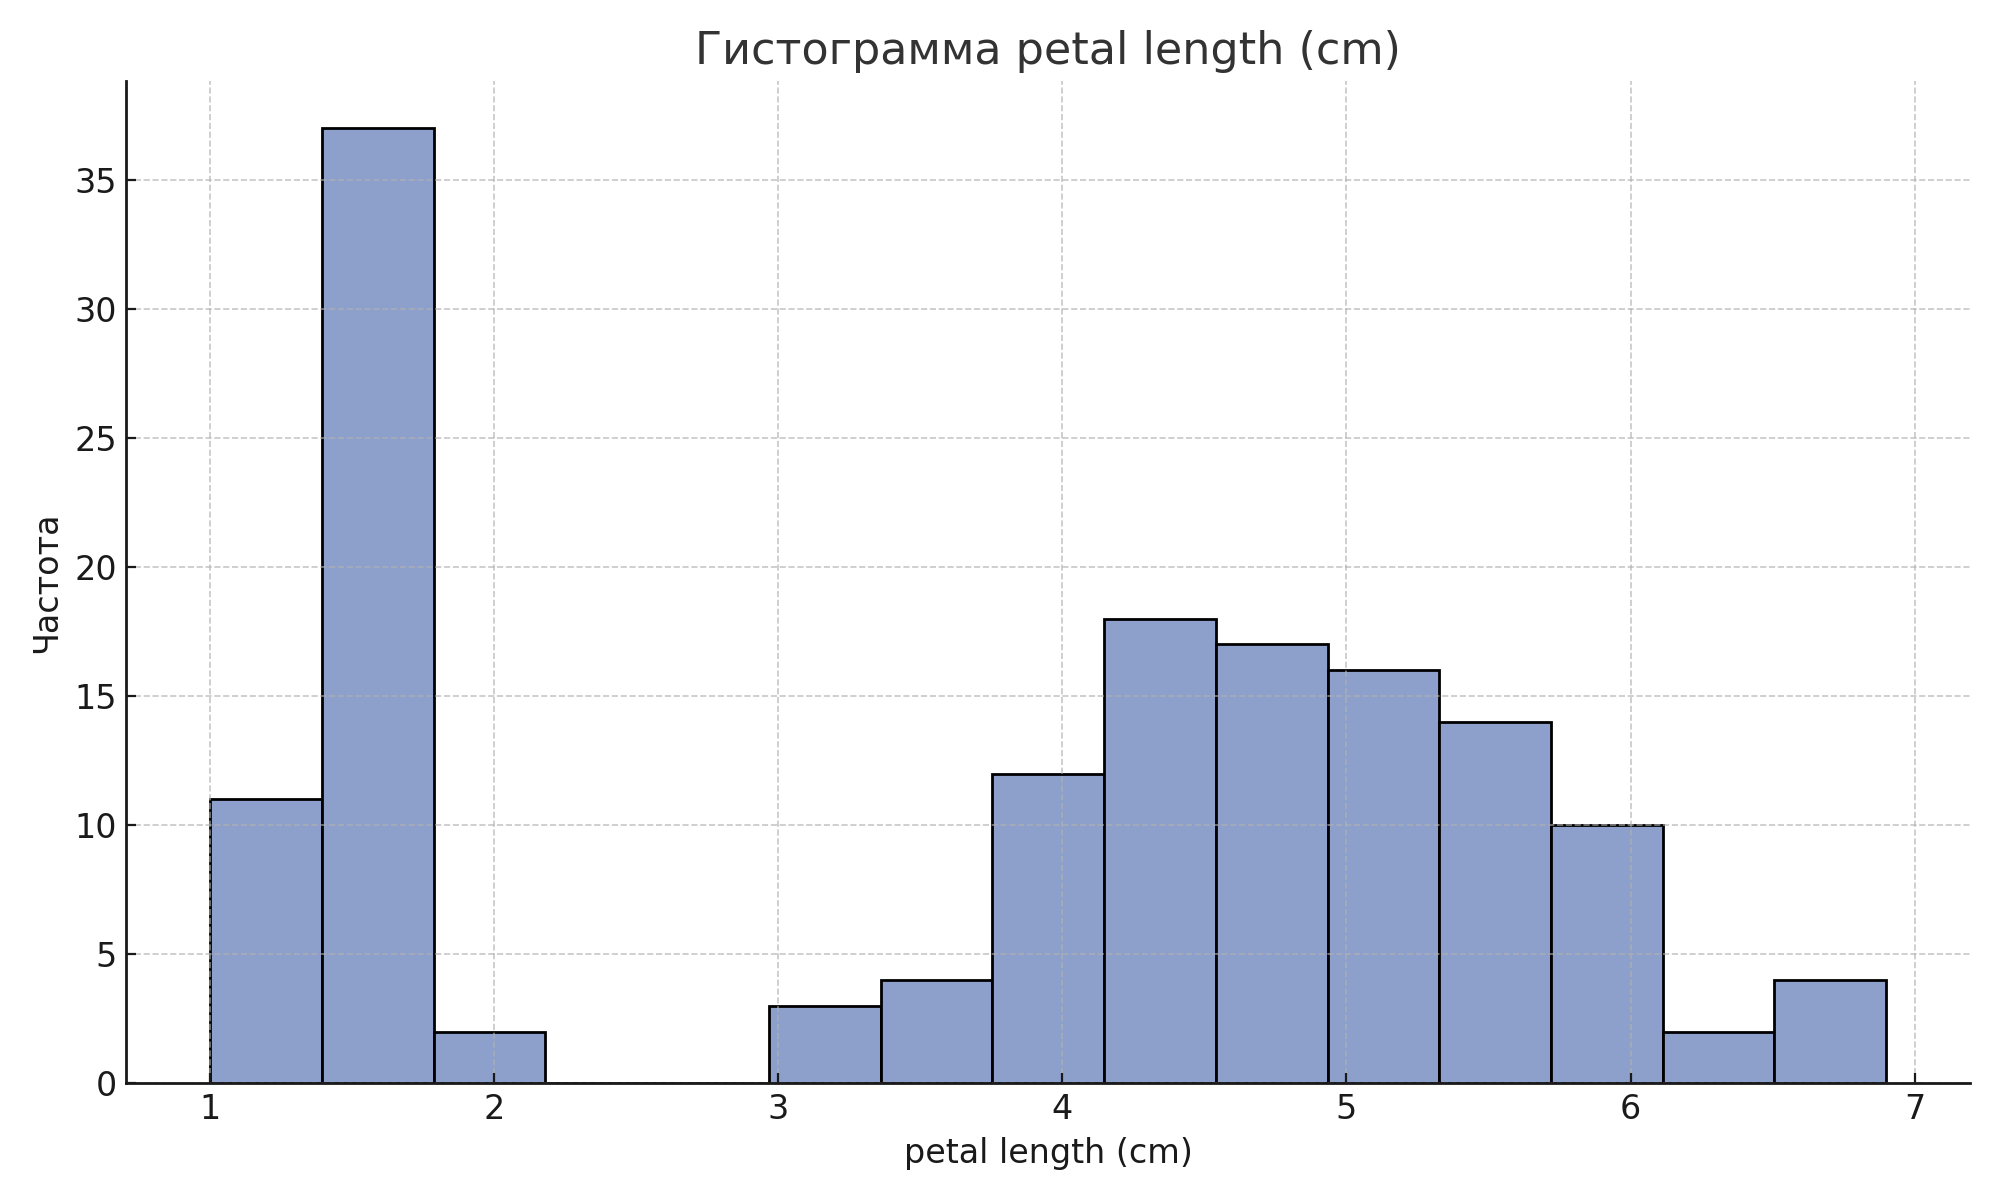
\includegraphics[width=0.8\textwidth]{images/histo_petal_length_cm_cb2.png}\\[6pt]
  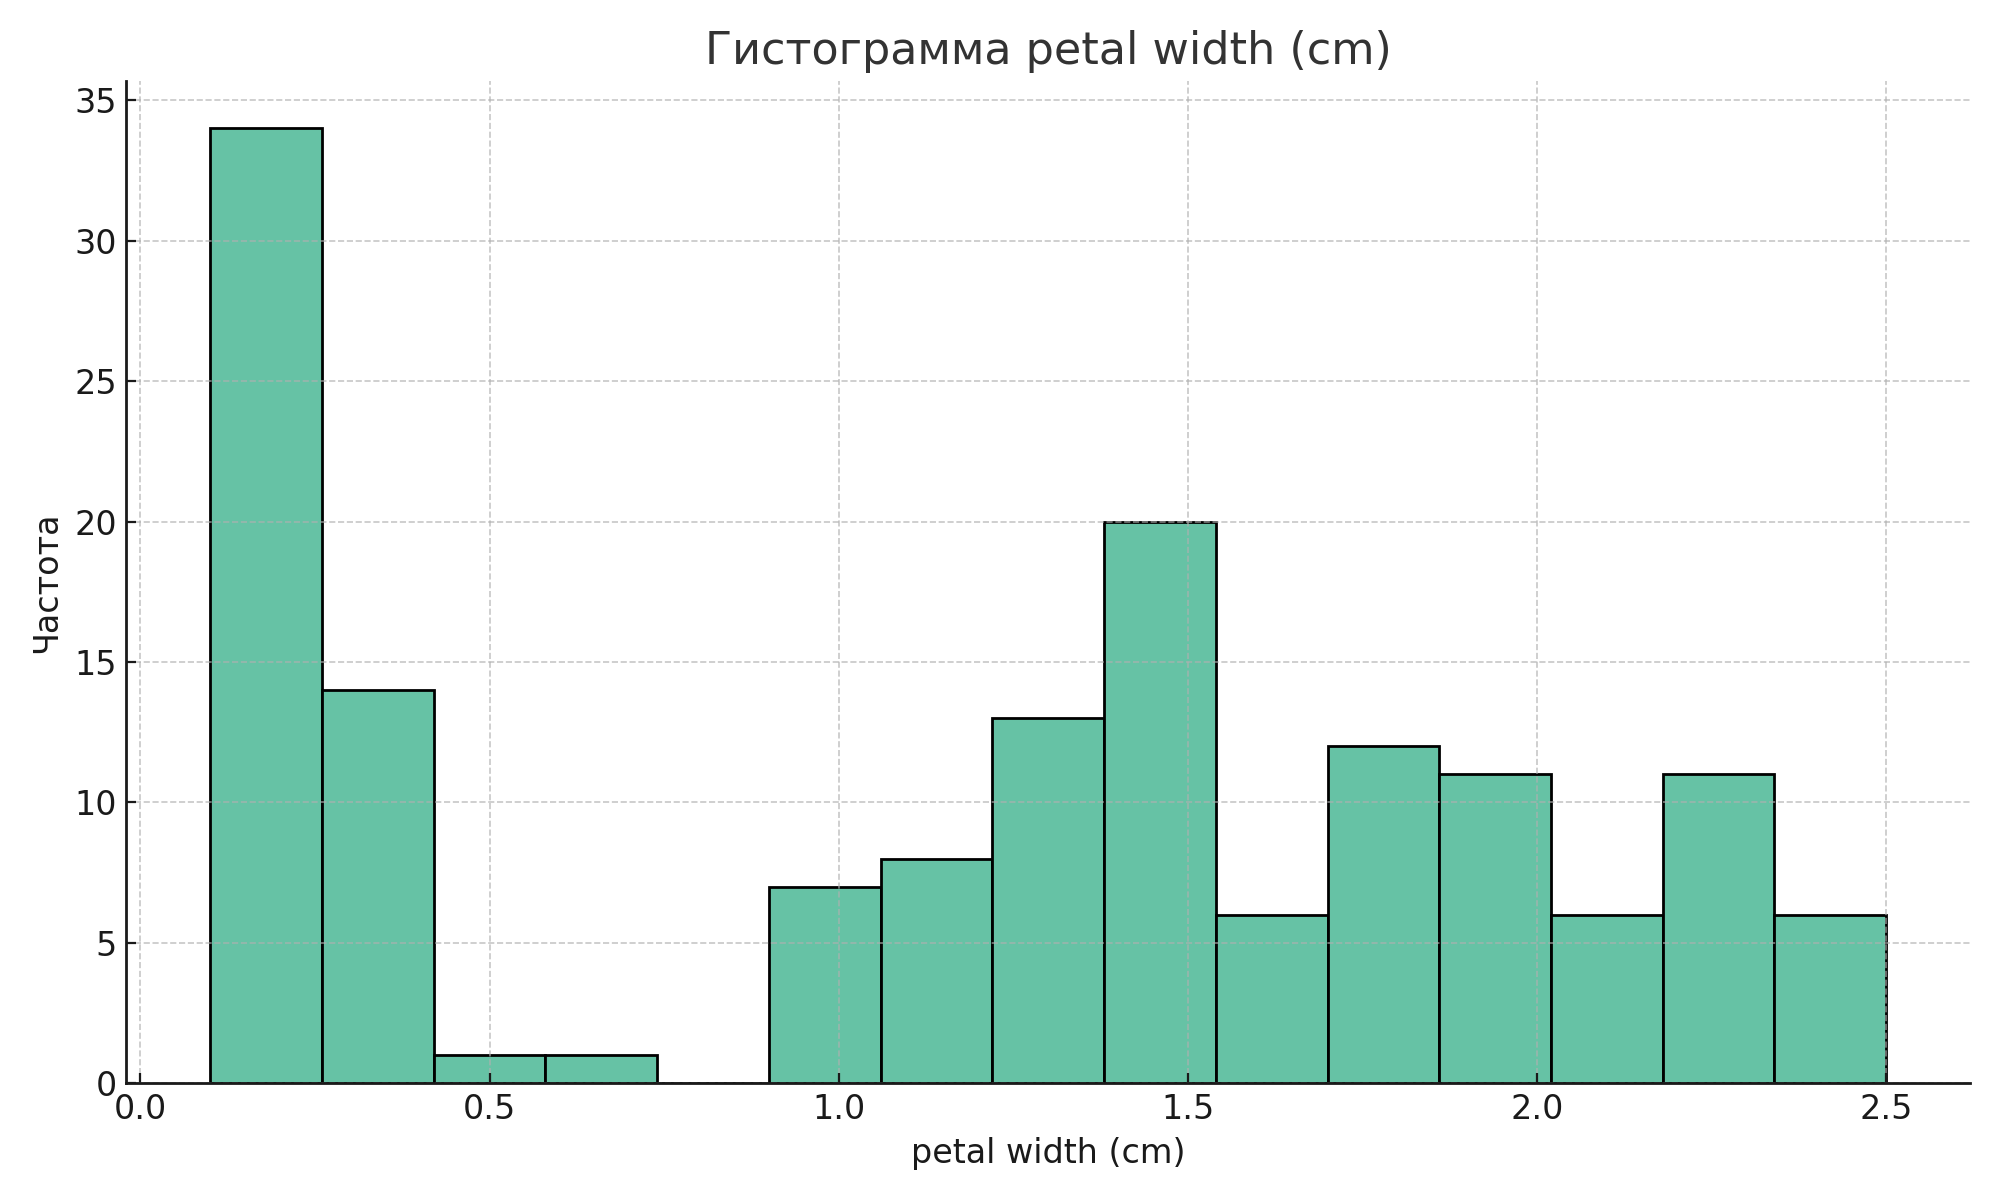
\includegraphics[width=0.8\textwidth]{images/histo_petal_width_cm_cb2.png}
  % не вызываем \caption — подпись продолжится от предыдущего блока
\end{figure}

\paragraph{Выводы.}
\begin{itemize}
  \item \textbf{sepal length} демонстрирует почти нормальное распределение с лёгкой дву­пиковостью (Setosa vs.~остальные виды).
  \item \textbf{sepal width} скошено вправо, большинство значений в [2.5, 3.5] см.
  \item \textbf{petal length} и \textbf{petal width} отчётливо мультимодальны: Setosa образует узкий «низ» (1–2 см), Versicolor и Virginica смещены вправо.
\end{itemize}

\subsubsection{Boxplot–анализ по видам}

Распределения по классам показаны на рис.~\ref{fig:iris_boxplots_vertical}.
\begin{figure}[H]
  \centering
  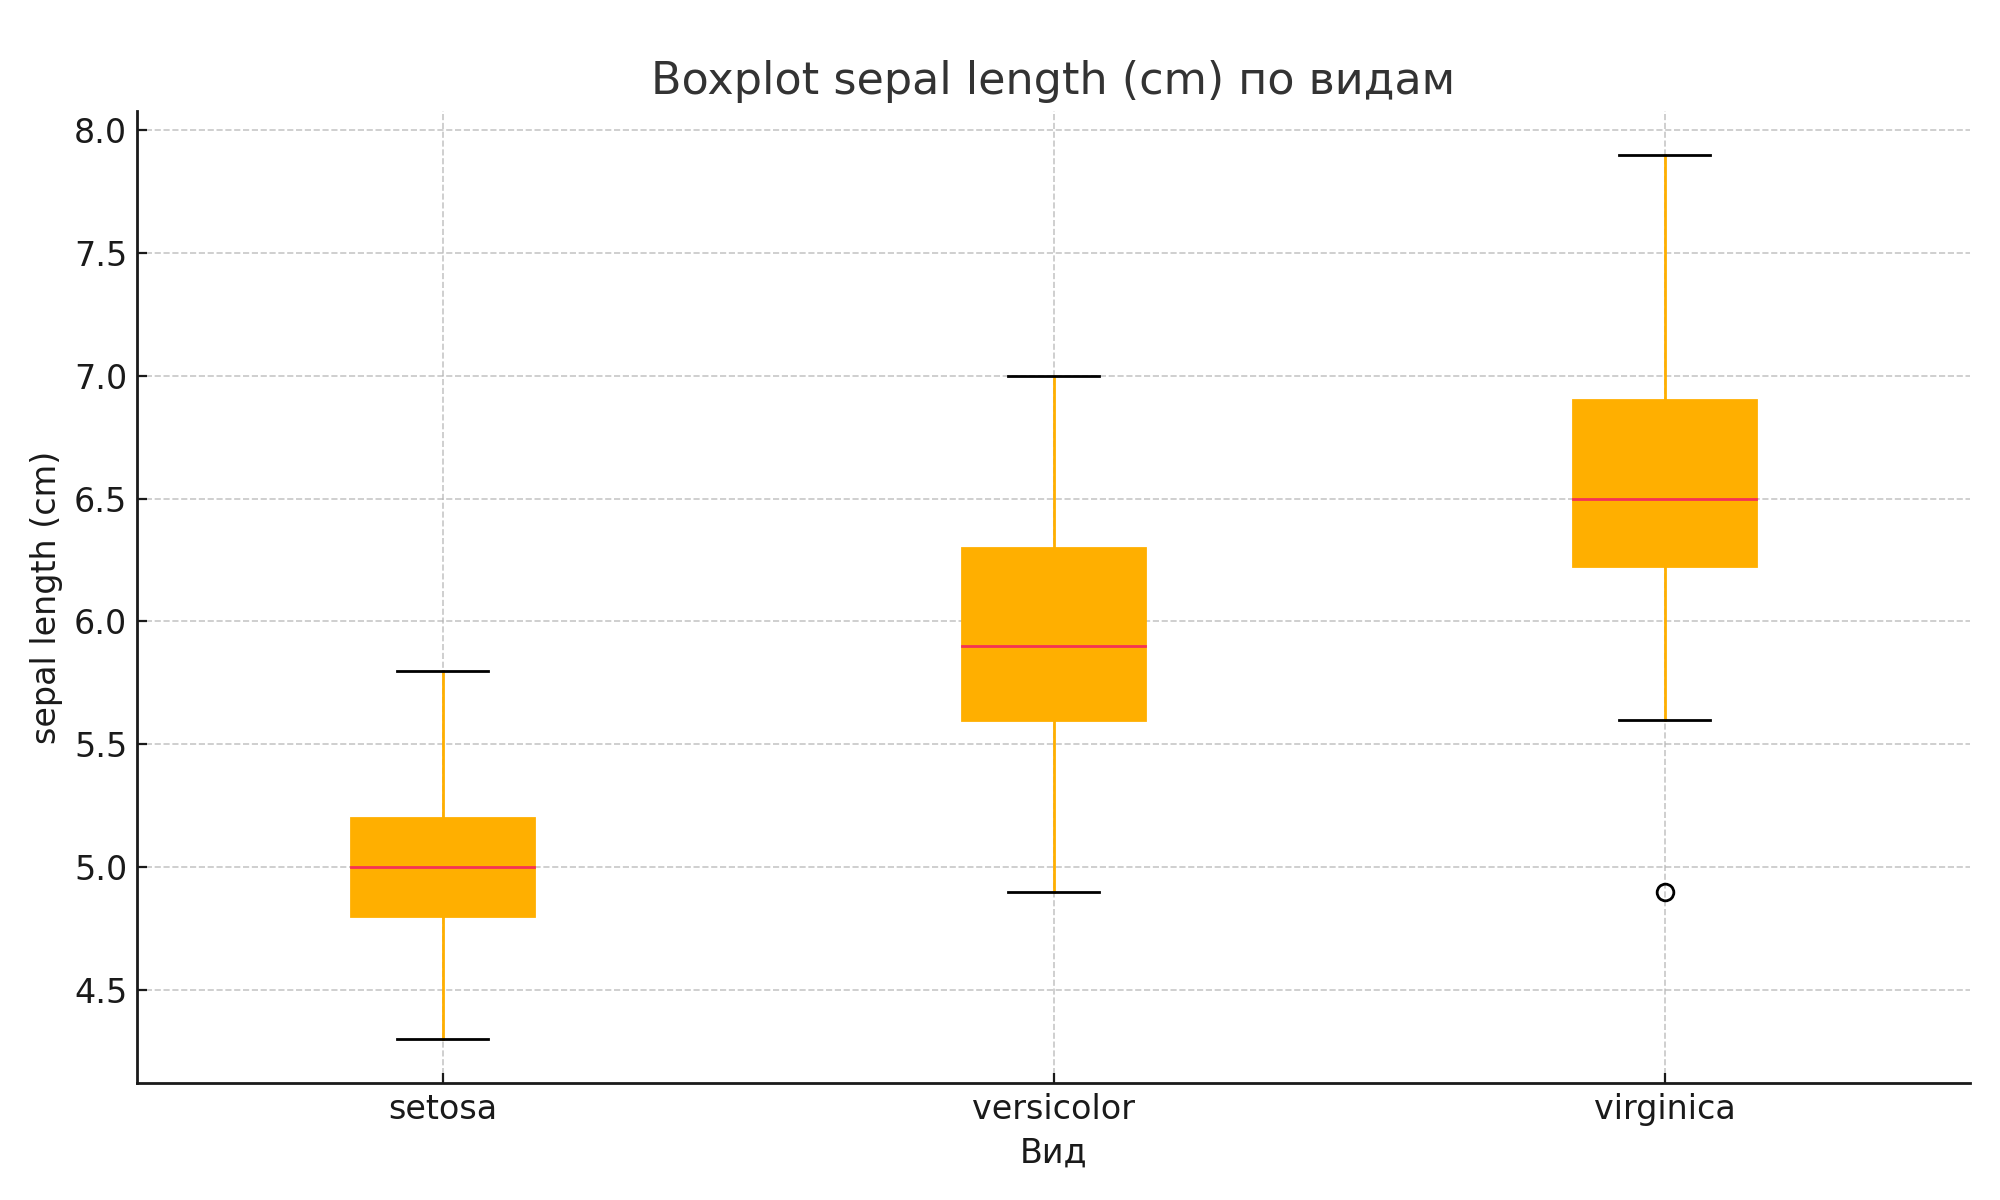
\includegraphics[width=0.8\textwidth]{images/box_sepal_length_cm_cb2.png}\\[6pt]
  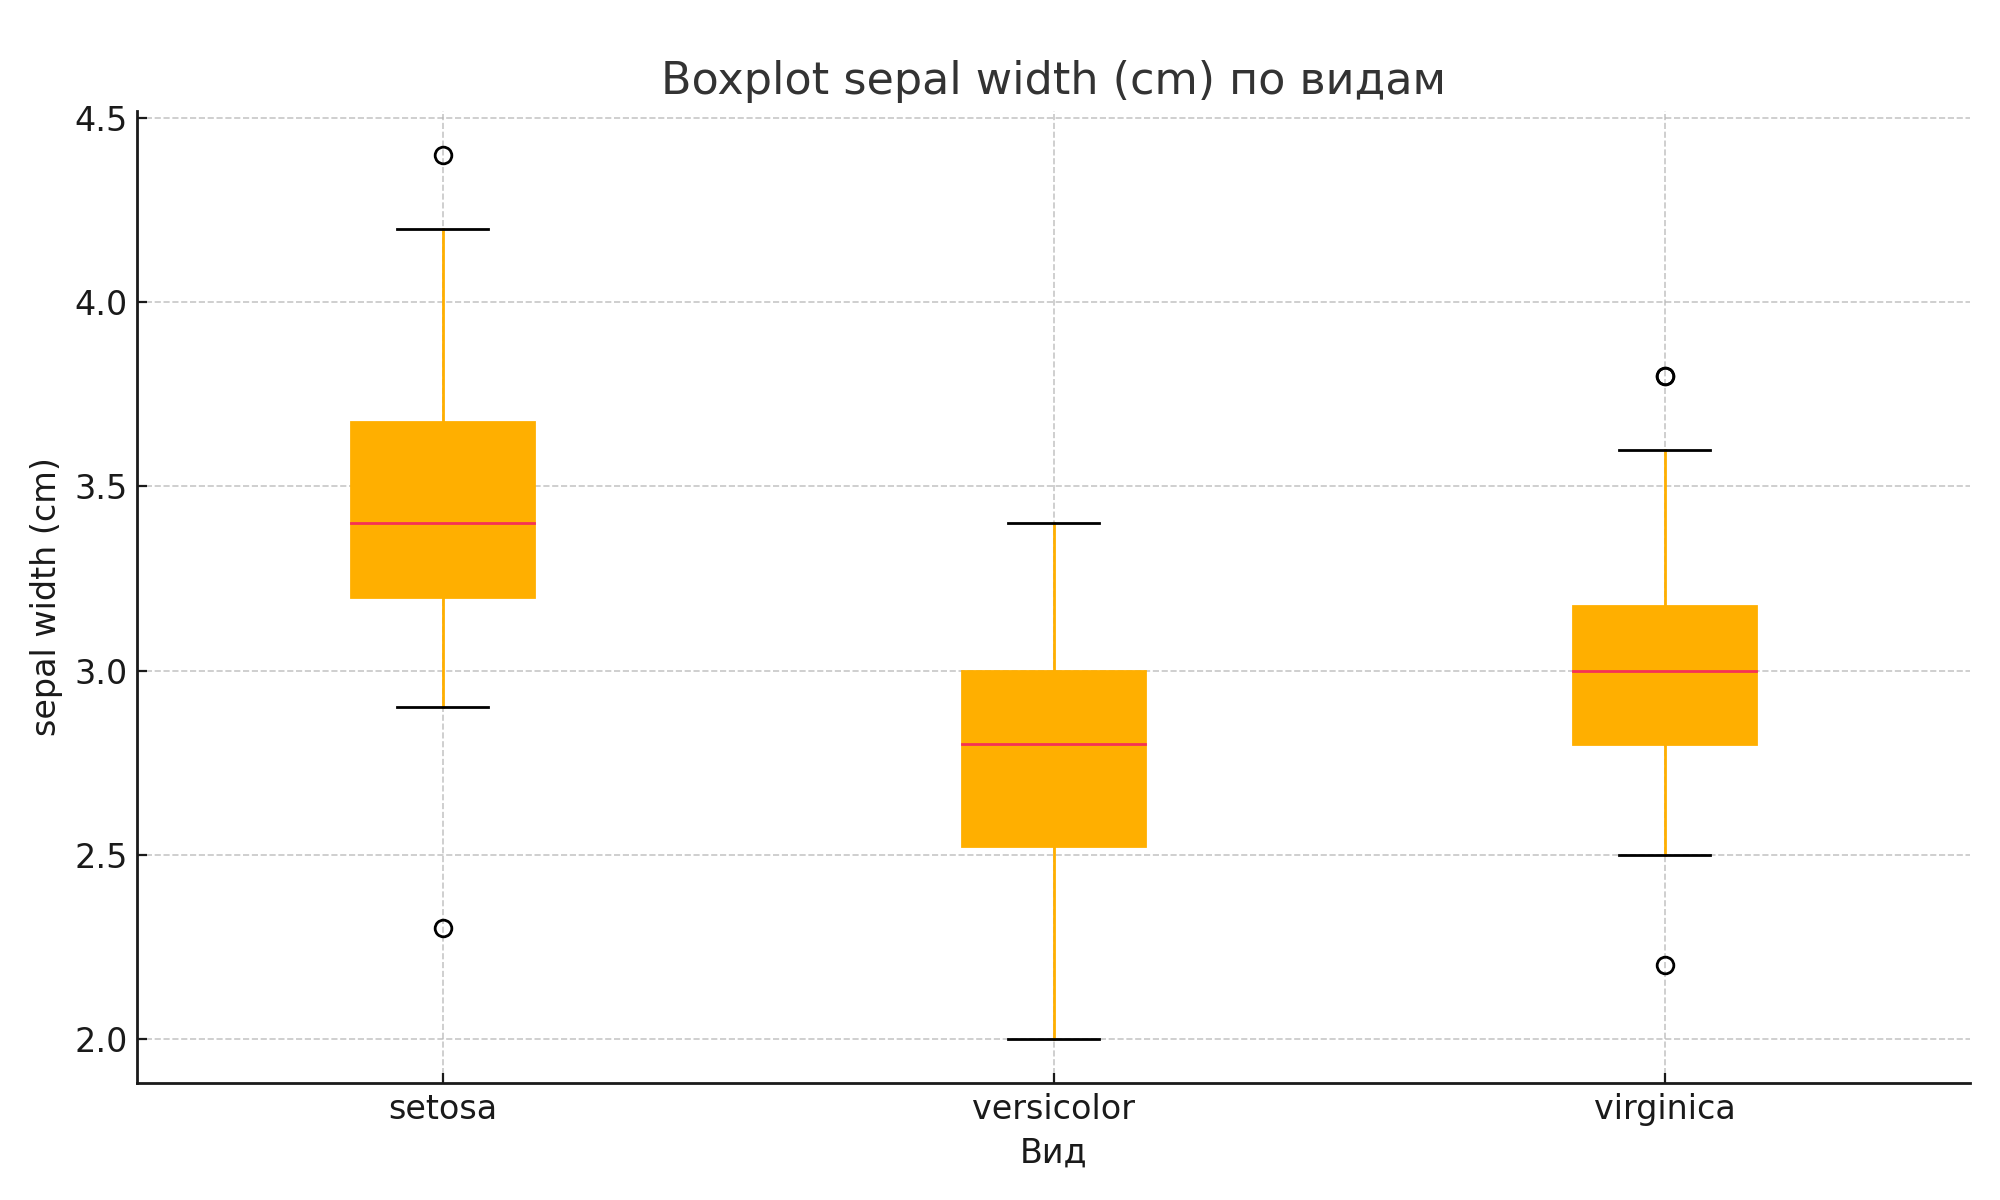
\includegraphics[width=0.8\textwidth]{images/box_sepal_width_cm_cb2.png}
  \caption{Boxplot–диаграммы признаков по видам Iris Dataset.}
  \label{fig:iris_boxplots_vertical}
\end{figure}

\begin{figure}[H]
  \ContinuedFloat
  \centering
  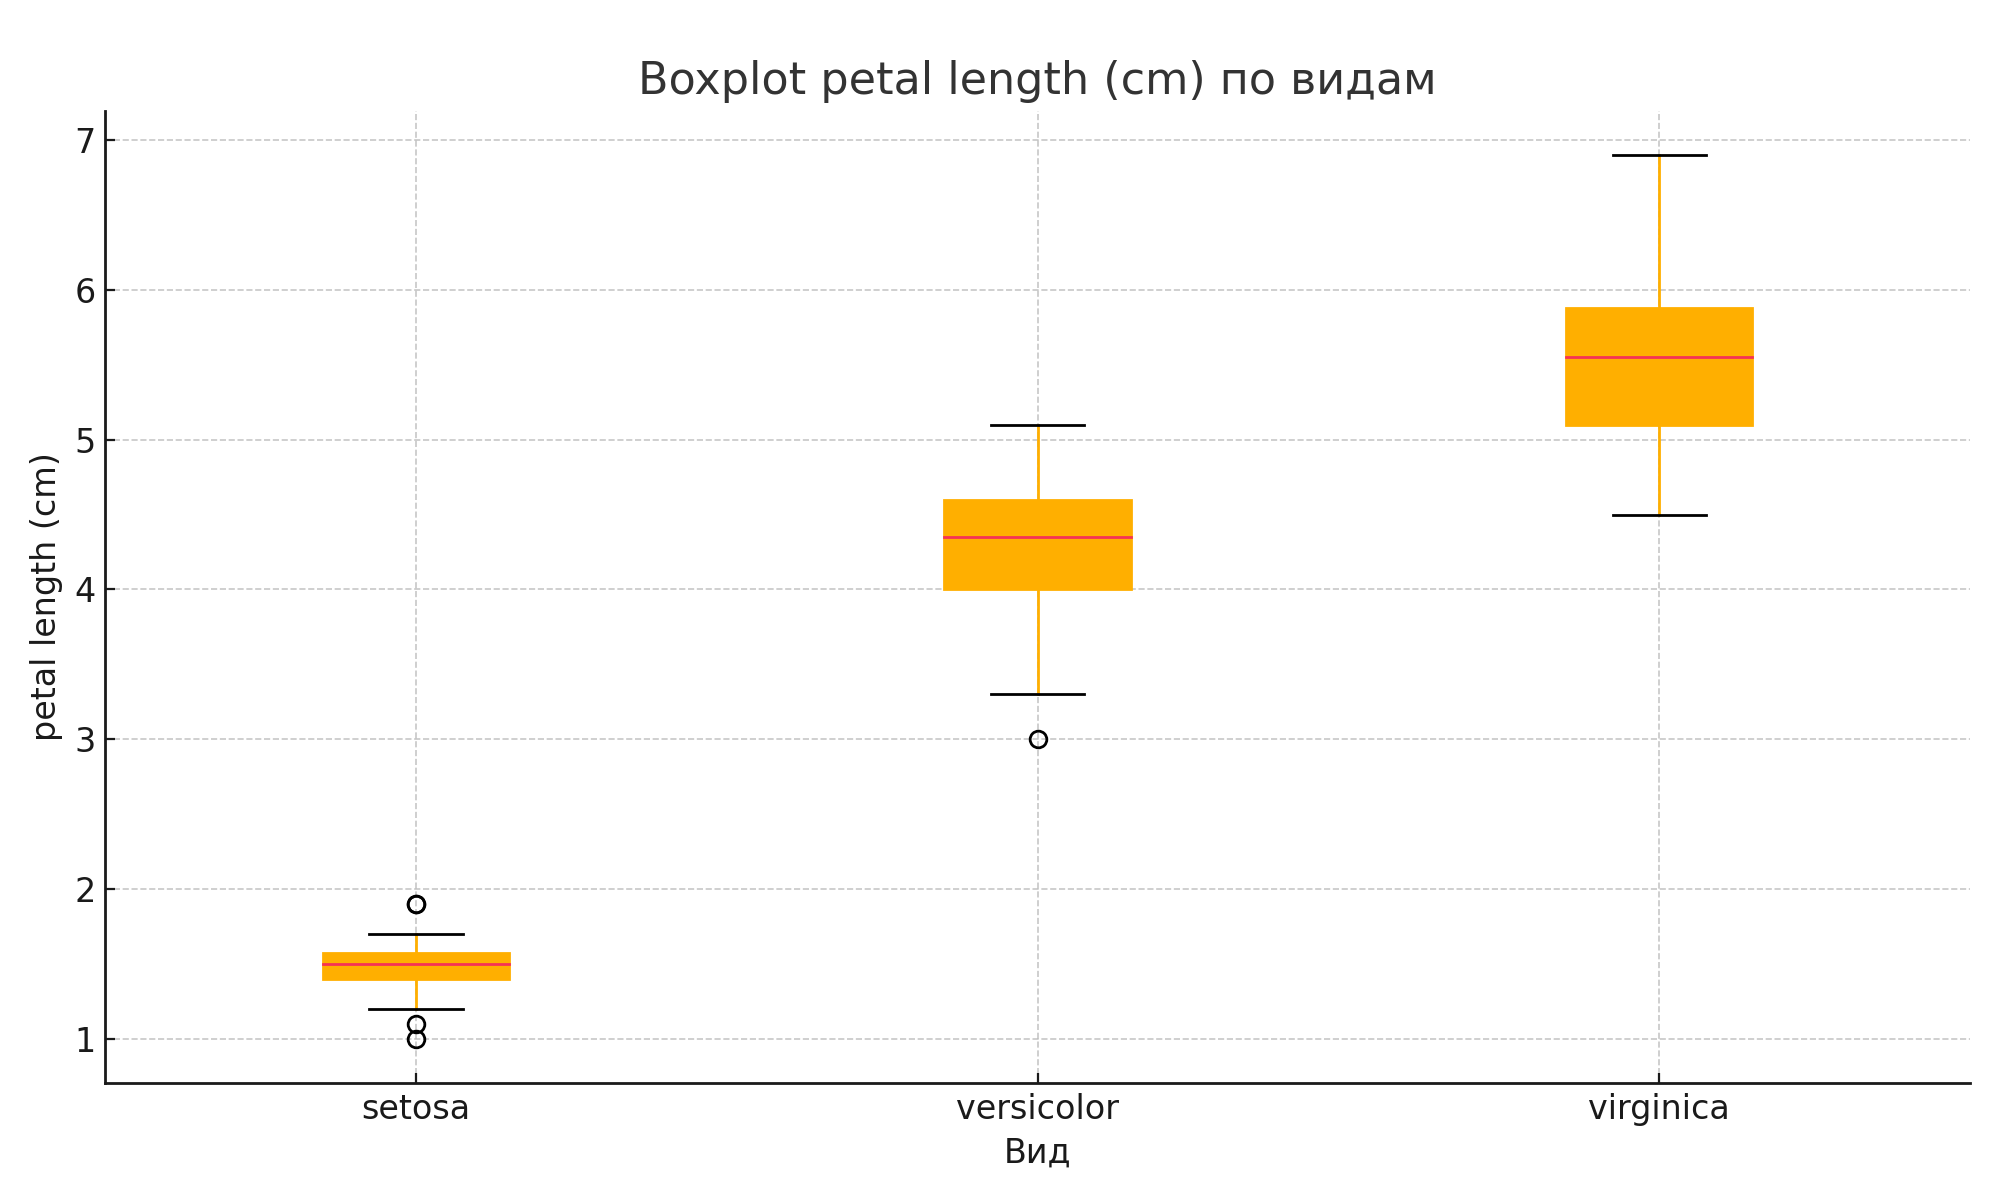
\includegraphics[width=0.8\textwidth]{images/box_petal_length_cm_cb2.png}\\[6pt]
  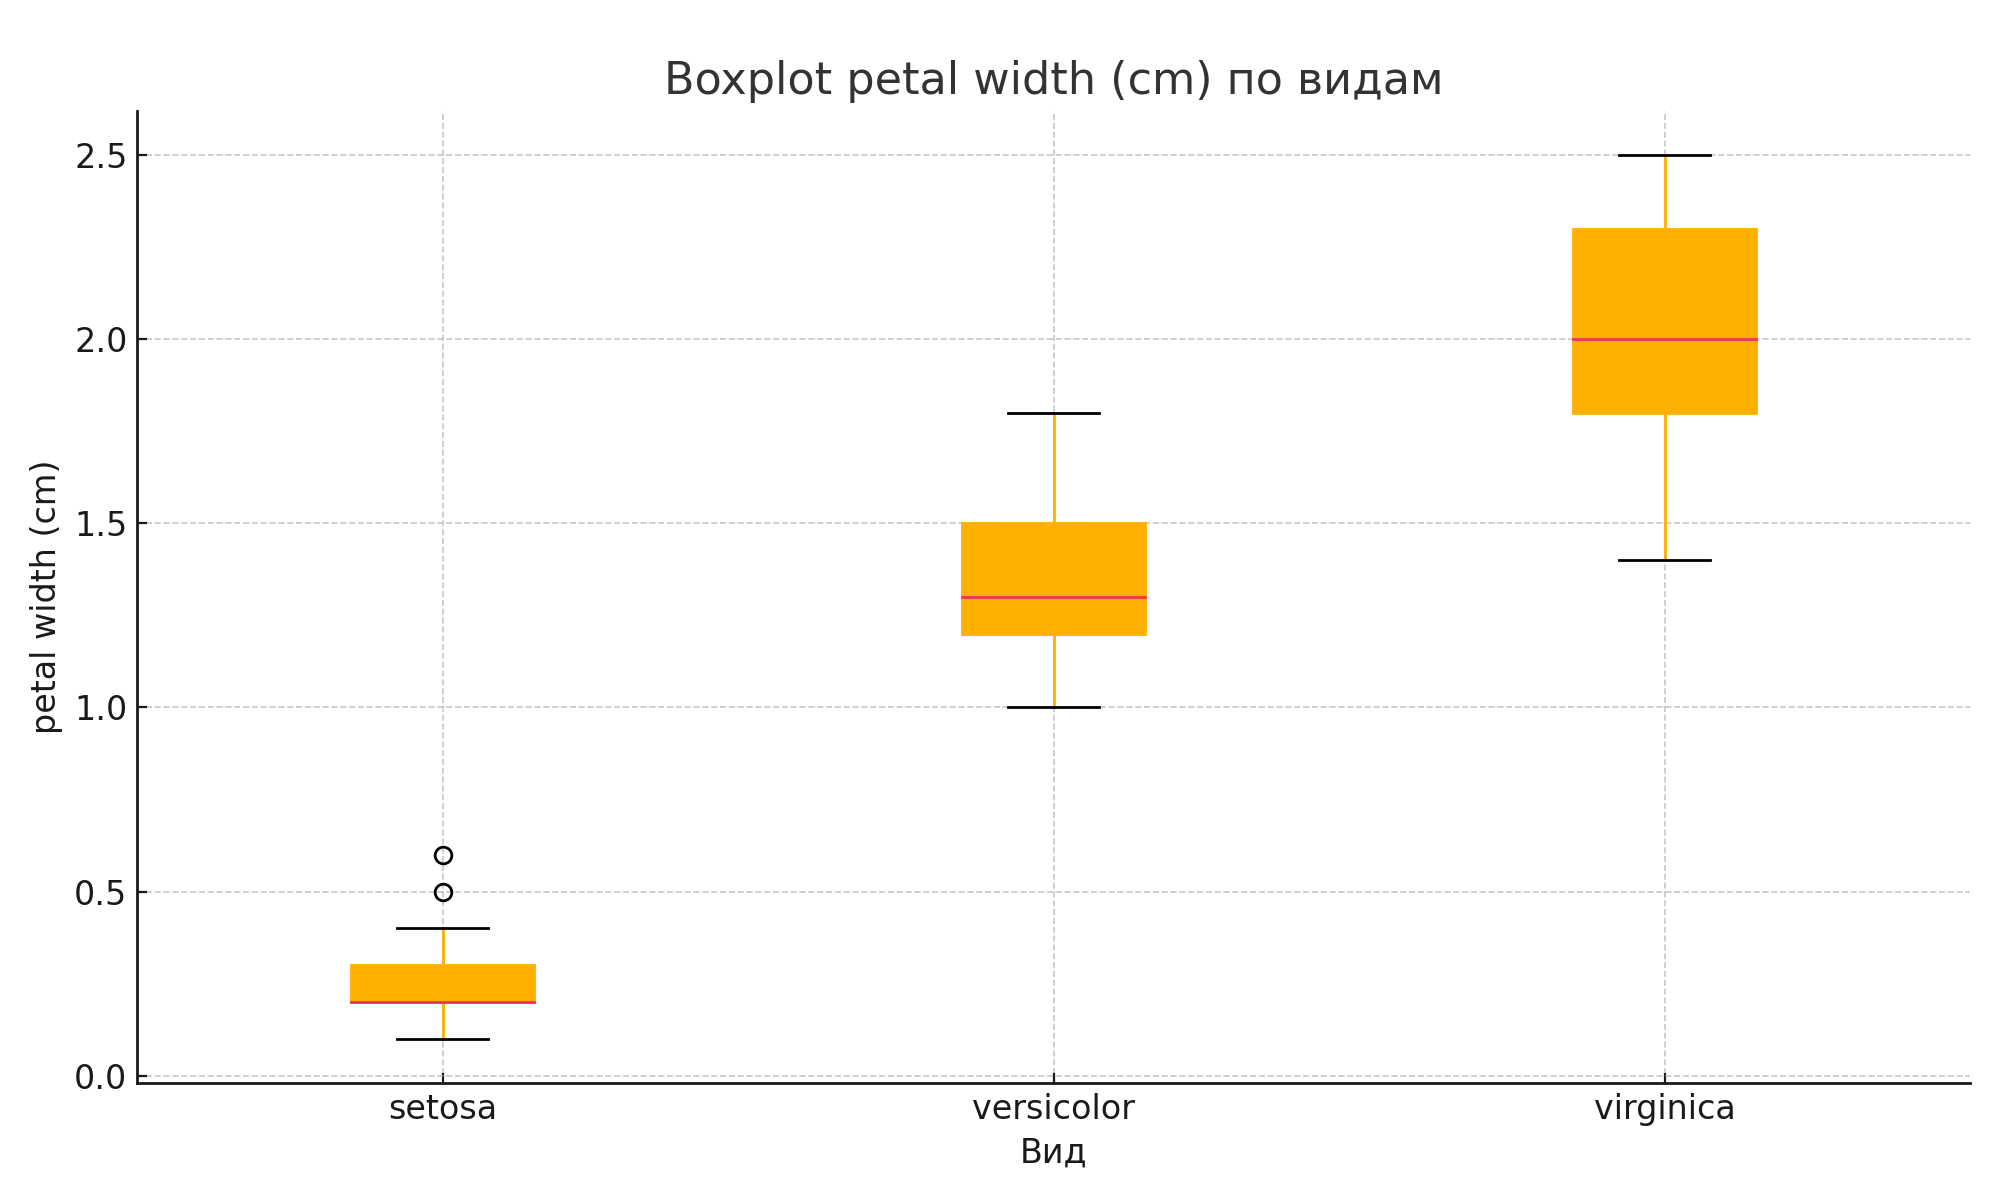
\includegraphics[width=0.8\textwidth]{images/box_petal_width_cm_cb2.png}
  \caption{Boxplot–диаграммы признаков по видам Iris Dataset.}
\end{figure}

\paragraph{Выводы.}
\begin{itemize}
  \item Для \emph{petal length/width} квартильные интервалы видов не перекрываются → признаки почти идеальны для классификации.
  \item Для \emph{sepal length/width} наблюдаются пересечения квартилей Versicolor и Virginica, поэтому они менее информативны в отрыве от лепестковых.
\end{itemize}

\subsubsection{Парная визуализация (Scatter–matrix)}

На рис.~\ref{fig:scatter_matrix} приведена матрица рассеяния всех пар признаков.

\begin{figure}[ht]
  \centering
  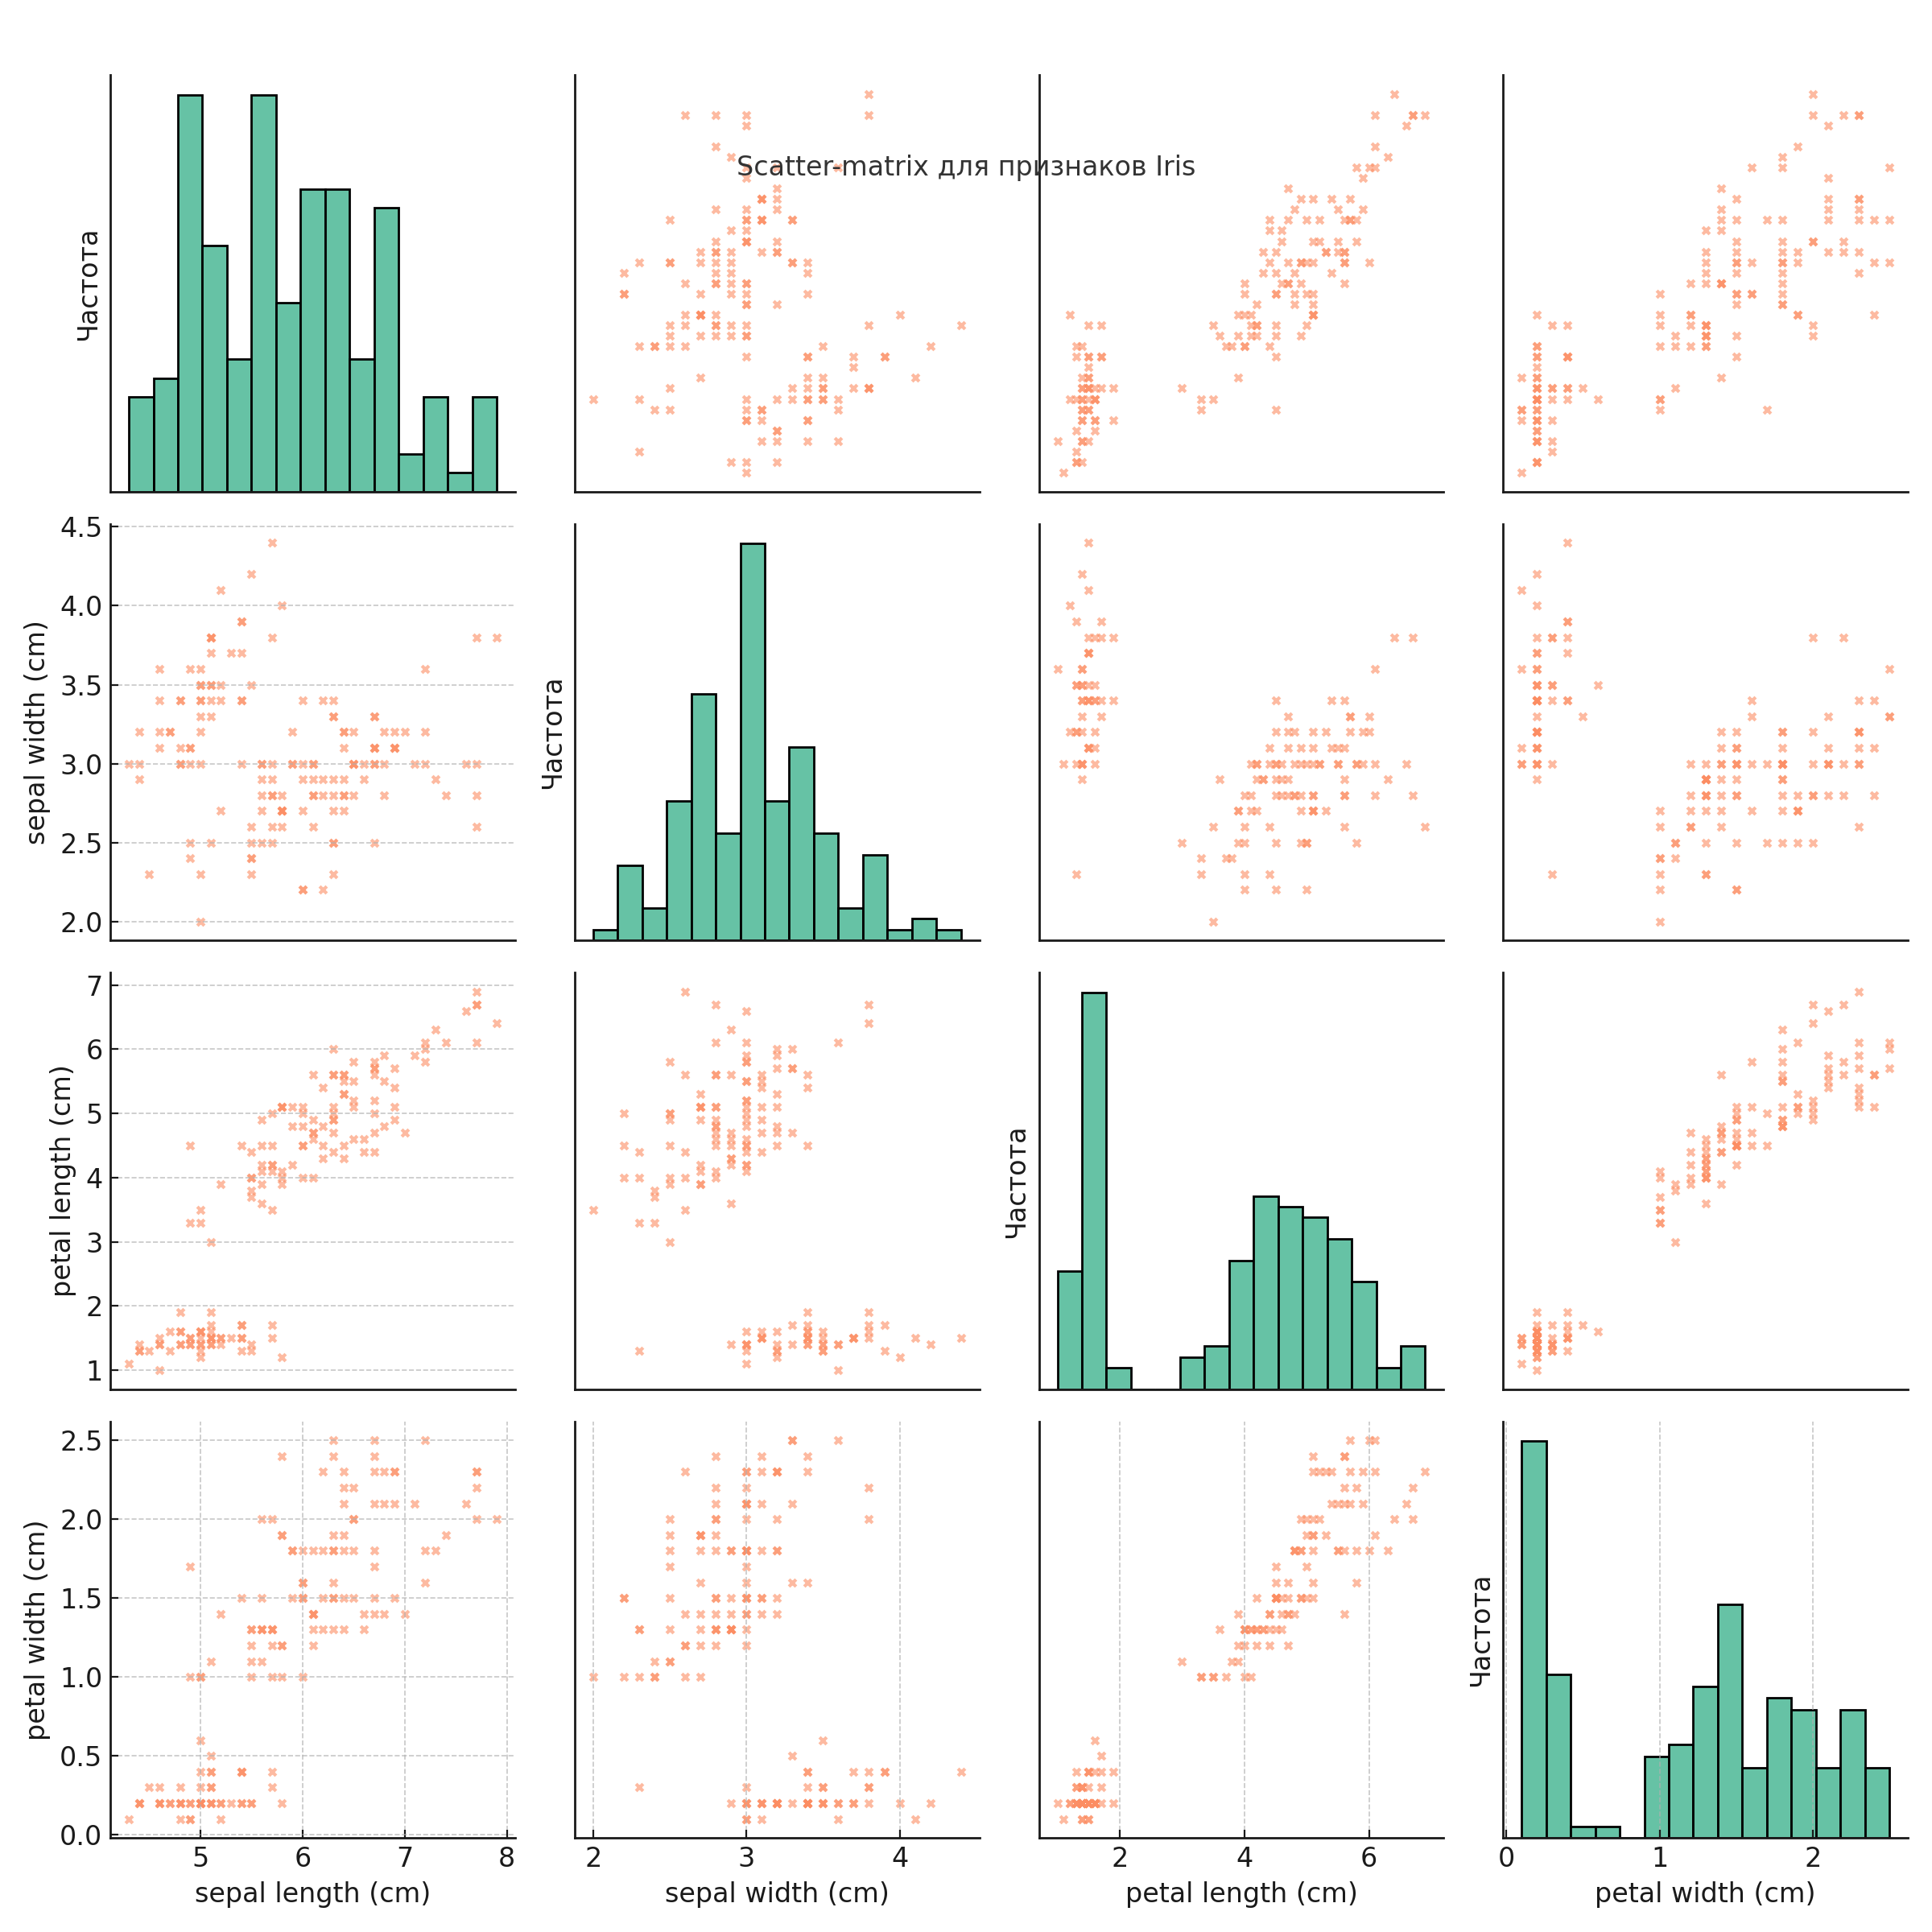
\includegraphics[width=\textwidth]{images/scatter_matrix_cb2.png}
  \caption{Scatter–matrix для признаков Iris.}
  \label{fig:scatter_matrix}
\end{figure}

\paragraph{Выводы.}
\begin{itemize}
  \item Самая сильная корреляция между \emph{petal length} и \emph{petal width}.
  \item Комбинации (\emph{sepal length}, \emph{petal length}) и (\emph{petal length}, \emph{petal width}) дают линейно разделимые классы.
  \item Пара (\emph{sepal width}, \emph{sepal length}) менее информативна.
\end{itemize}

\subsubsection{Кластеризация K–Means}

Наконец, на рис.~\ref{fig:kmeans_cb2} представлена K–Means кластеризация ($k=3$) по паре (\emph{sepal length}, \emph{petal length}), использующая ту же палитру ColorBrewer\_2.

\begin{figure}[ht]
  \centering
  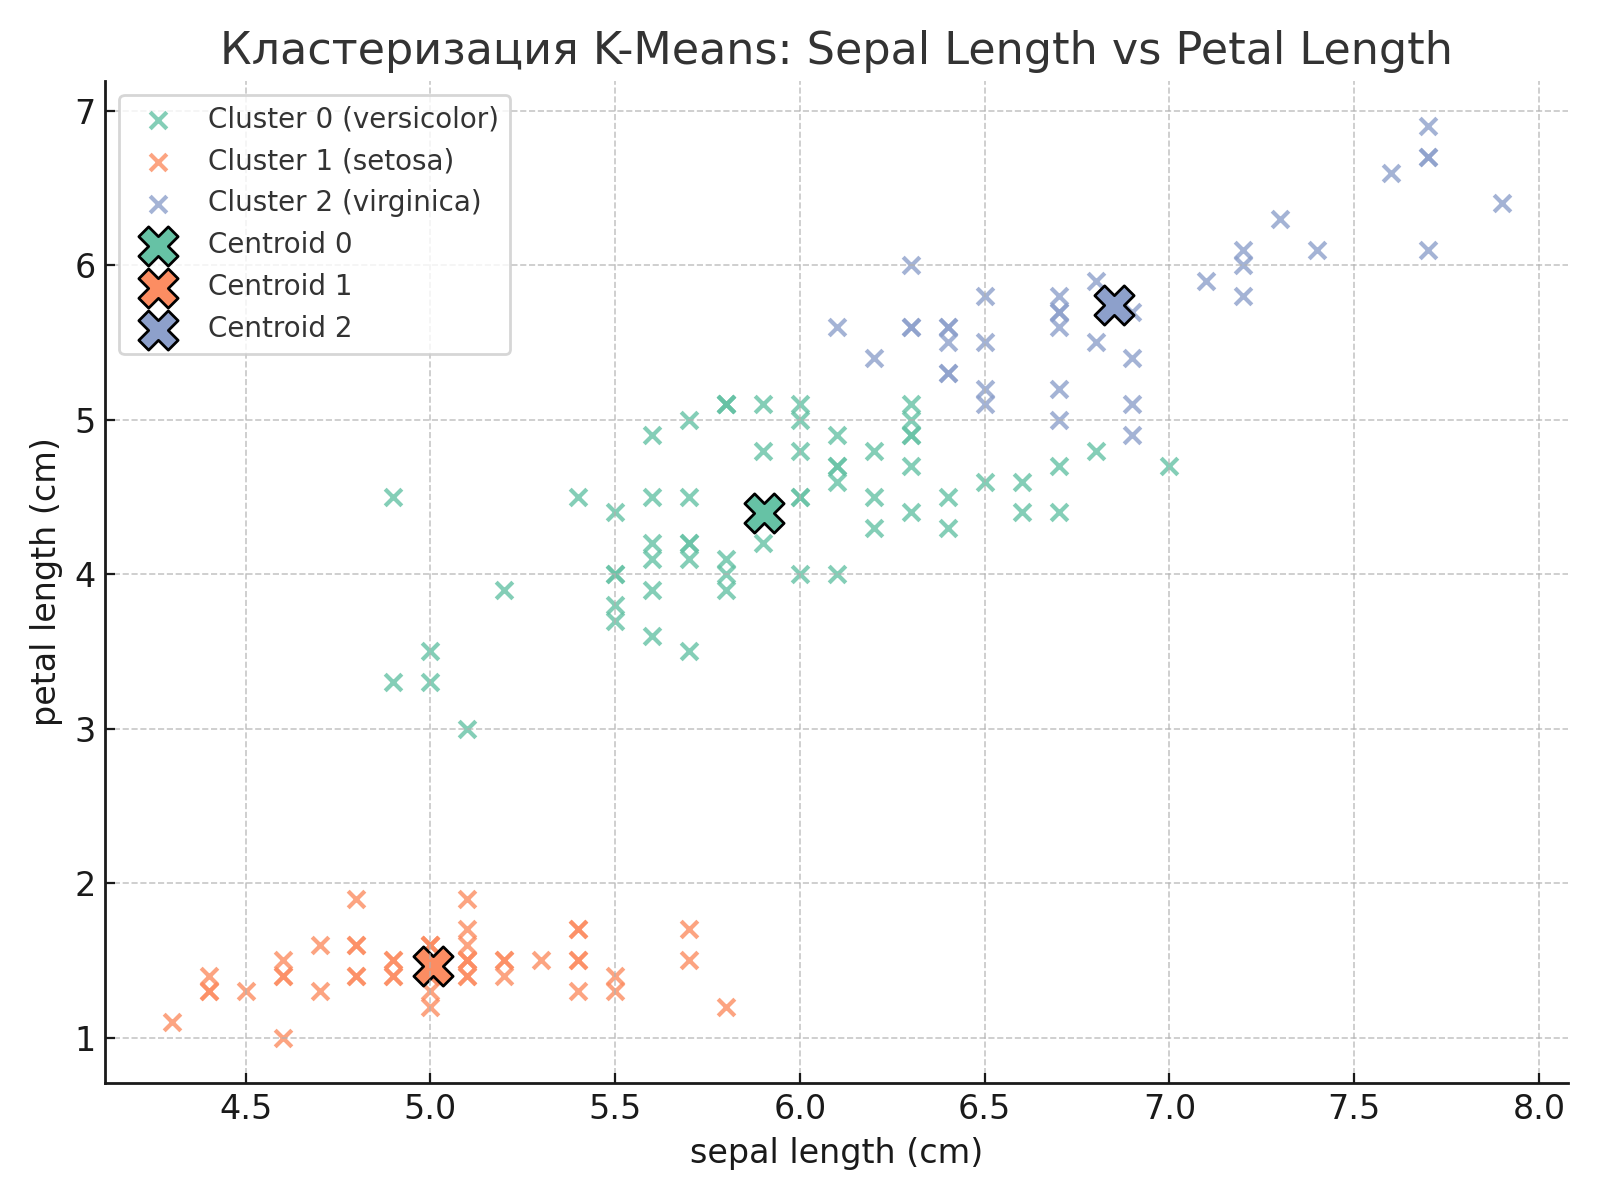
\includegraphics[width=0.8\textwidth]{images/cluster_plot_cb2.png}
  \caption{Кластеризация K–Means: Sepal Length vs Petal Length. Кластеры подписаны с указанием доминирующего вида; центроиды отмечены крупными крестами.}
  \label{fig:kmeans_cb2}
\end{figure}

\paragraph{Выводы.}
\begin{itemize}
  \item \textbf{Cluster 1 (setosa)}: полностью отделён в нижнем левом углу, петаловые признаки минимальны — 100\% точность.
  \item \textbf{Cluster 0 (versicolor)}: средняя область, 48 из 50 экземпляров Versicolor точно отделены (96\%); 14 Virginica попали в этот кластер из–за близости.
  \item \textbf{Cluster 2 (virginica)}: правый верхний угол, 36 из 50 Virginica (72\%), несколько Versicolor «зашли» внутрь.
  \item Итог: лепестковые признаки дают главную разделительную информацию, чашелистики лишь уточняют границы.
\end{itemize}

\addcontentsline{toc}{section}{СПИСОК ЛИТЕРАТУРЫ} % и добавляем её в оглавление, если требуется
\ESKDsignature{\normalsize Список литературы}
\eskdrerun{}

\begin{thebibliography}{200}
\bibitem{Kulabukhov2023}
С.\,В.~Кулабухов.
\newblock Разработка методов анализа данных на основе мягких вычислений
  с использованием нечеткого значения истинности.
\newblock Кандидатская диссертация, БГТУ им.~В.\,Г.~Шухова, Белгород, 2023.

\bibitem{SinukPivnenko2006}
В.\,Г.~Синюк, Е.\,В.~Пивненко.
\newblock Об аналитическом вычислении нечеткого значения истинности.
\newblock В сб.: Нечеткие системы, мягкие вычисления и интеллектуальные технологии (НСМВ-2006), Физматлит, М., 2006, с.~129–133.
\bibitem{Zadeh1965}
  Заде Л.~А. \emph{Fuzzy sets} // Information and Control. 1965. Т.~8, №~3. С.~338--353.
\bibitem{Mamdani1975}
  Мамдани Э.~Х., Ассилиан С. \emph{An experiment in linguistic synthesis with a fuzzy logic controller} // International Journal of Man-Machine Studies. 1975. Т.~7, №~1. С.~1--13.
\bibitem{Ross2004}
  Росс Т.~Дж. \emph{Fuzzy Logic with Engineering Applications}. Chichester: John Wiley \& Sons, 2004. 576 с.
\bibitem{Zadeh1975}
  Заде Л.~А. \emph{The concept of a linguistic variable and its application to approximate reasoning—I} // Information Sciences. 1975. Т.~8, №~4. С.~199--249.
\bibitem{Sugeno1985}
  Сугено М. \emph{Industrial applications of fuzzy control} // Fuzzy Sets and Systems. 1985. Т.~29, №~1. С.~47--52.
\bibitem{Jang1993}
  Джанг Дж.-С.~Р. \emph{ANFIS: Adaptive-Network-Based Fuzzy Inference System} // IEEE Trans. Syst., Man, and Cybernetics. 1993. Т.~23, №~3. С.~665--685.
\bibitem{Wang1992}
  Ван Л.-Х., Мендель Дж.-М. \emph{Generating fuzzy rules by learning from examples} // IEEE Trans. Syst., Man, and Cybernetics. 1992. Т.~22, №~6. С.~1414--1427.
\bibitem{Bezdek1981}
  Бездек Дж.~К. \emph{Pattern Recognition with Fuzzy Objective Function Algorithms}. New York: Plenum Press, 1981. 271 с.

\bibitem{Zadeh1965}
L.\,A.~Zadeh.
\newblock Fuzzy Sets.
\newblock {\em Information and Control}, 8(3):338–353, 1965.

\bibitem{KlirYuan1995}
G.\,J.~Klir, B.\,Y.~Yuan.
\newblock Fuzzy Sets and Fuzzy Logic: Theory and Applications.
\newblock Prentice Hall, 1995.

\bibitem{Ross2010}
T.~J.~Ross.
\newblock Fuzzy Logic with Engineering Applications.
\newblock Wiley, 2010.

\bibitem{Mendel2001}
J.\,M.~Mendel.
\newblock Uncertain Rule-Based Fuzzy Logic Systems: Introduction and New Directions.
\newblock Prentice Hall PTR, 2001.

\bibitem{Zimmermann2001}
H.--J.~Zimmermann.
\newblock Fuzzy Set Theory—and Its Applications.
\newblock Kluwer Academic, 2001.

\bibitem{DuboisPrade1988}
D.~Dubois, H.~Prade.
\newblock Possibility Theory: An Approach to Computerized Processing of Uncertainty.
\newblock Plenum Press, 1988.

\bibitem{Abe2001}
S.~Abe.
\newblock Fuzzy Logic for Engineering Applications.
\newblock Springer, 2001.

\bibitem{Mamdani1974}
E.\,H.~Mamdani.
\newblock Applications of Fuzzy Algorithms for Simple Dynamic Plants.
\newblock {\em Proceedings of the IEEE}, 121(1):1585–1588, 1974.

\bibitem{TakagiSugeno1985}
T.~Takagi, M.~Sugeno.
\newblock Fuzzy Identification of Systems and Its Applications to Modeling and Control.
\newblock {\em IEEE Trans. Systems, Man, and Cybernetics}, SMC-15(1):116–132, 1985.

\bibitem{YagerFilev1994}
R.\,R.~Yager, D.\,P.~Filev.
\newblock Essentials of Fuzzy Modeling and Control.
\newblock Wiley, 1994.

\bibitem{Pedrycz1996}
W.~Pedrycz.
\newblock Fuzzy Neural Networks: Architectures, Strategies and Applications.
\newblock Kluwer, 1996.

\bibitem{KacprzykFedrizzi1990}
J.~Kacprzyk, M.~Fedrizzi (eds.).
\newblock Fuzzy Sets in Decision Analysis, Operations Research and Statistics.
\newblock Springer, 1990.

\bibitem{NguyenWalker1999}
H.\,T.~Nguyen, E.\,A.~Walker.
\newblock A First Course in Fuzzy Logic.
\newblock CRC Press, 1999.

\bibitem{Bonissone1999}
P.\,P.~Bonissone.
\newblock Fuzzy Logic: A Spectrum of Methods and Applications.
\newblock In {\em Fuzzy Logic: State of the Art}, Kluwer, 1999.

\bibitem{DuboisPrade2012}
D.~Dubois, H.~Prade.
\newblock Abe Mamdani: A Pioneer of Soft Artificial Intelligence.
\newblock In {\em Combining Experimentation and Theory}, Springer, 2012.

\bibitem{CingolaniAlcala2012}
P.~Cingolani, J.~Alcalá-Fdez.
\newblock JFuzzyLogic: A Robust and Flexible Fuzzy-Logic Inference System.
\newblock {\em IEEE International Conference on Fuzzy Systems}, 2012.

\bibitem{RadaVilela2019}
J.~Rada-Vilela.
\newblock Fuzzylite: a Fuzzy Logic Control Library.
\newblock Available at: \url{http://www.fuzzylite.com} (accessed 11.06.2019).

\bibitem{Cordon2004}
O.~Cordón et al.
\newblock Evolutionary Adaptive Defuzzification Methods in Fuzzy Modeling.
\newblock {\em Int. Journal of Hybrid Intelligent Systems}, 1(2):81–93, 2004.

\bibitem{AlsinaFrankSchweizer2006}
C.~Alsina, M.\,J.~Frank, B.~Schweizer.
\newblock Associative Functions: Triangular Norms and Copulas.
\newblock World Scientific, 2006.

\bibitem{BaczynskiJayaram2008}
M.~Baczyński, V.~Jayaram.
\newblock Fuzzy Implications.
\newblock Springer, 2008.

\bibitem{Aliev2013}
R.\,A.~Aliev.
\newblock Fundamentals of the Fuzzy Logic-Based Generalized Theory of Decisions.
\newblock Springer, 2013.

\bibitem{SinukKulabukhov2022}
V.\,G.~Sinuk, S.\,V.~Kulabukhov.
\newblock Method for Classification of Objects with Fuzzy Values of Features.
\newblock {\em Information Technologies and Computing Systems}, 2022.

\bibitem{Rutkowski2004}
L.~Rutkowski.
\newblock Flexible Neuro-Fuzzy Systems: Structures, Learning and Performance Evaluation.
\newblock Kluwer, 2004.

\bibitem{Rutkowska2001}
D.~Rutkowska, L.~Rutkowski, R.~Nowicki.
\newblock Neuro-fuzzy systems with inference based on bounded product.
\newblock In {\em Advances in Neural Networks and Applications}, 2001.

\bibitem{MendelChimatapuHagras2020}
J.\,M.~Mendel, R.~Chimatapu, H.~Hagras.
\newblock Comparing the performance potentials of singleton and non-singleton fuzzy systems.
\newblock {\em IEEE Trans. on Fuzzy Systems}, 28(4):789–798, 2020.

\bibitem{Baldwin1980}
J.\,F.~Baldwin.
\newblock Feasible Algorithms for Approximate Reasoning Using Fuzzy Logic.
\newblock {\em Fuzzy Sets and Systems}, 4(1):17–38, 1980.

\bibitem{BorgesGracio2006}
F.~Borges, R.~Grácio.
\newblock A Tutorial on Interval Type-2 Fuzzy Sets.
\newblock {\em IEEE Trans. on Fuzzy Systems}, 14(3):354–370, 2006.

\bibitem{KlirFolger1988}
G.\,J.~Klir, T.\,A.~Folger.
\newblock Fuzzy Sets, Uncertainty, and Information.
\newblock Prentice Hall, 1988.

\bibitem{Kandel1986}
A.~Kandel.
\newblock Fuzzy Mathematical Techniques with Applications.
\newblock Addison-Wesley, 1986.

\bibitem{Zimmerman1991}
H.--J.~Zimmerman.
\newblock An Introduction to Fuzzy Logic and Fuzzy Sets.
\newblock Kluwer, 1991.

\bibitem{Bezdek1981}
J.\,C.~Bezdek.
\newblock Pattern Recognition with Fuzzy Objective Function Algorithms.
\newblock Springer, 1981.

\bibitem{BezdekKeller1999}
J.\,C.~Bezdek, J.\,M.~Keller, R.~Krishnapuram, N.\,R.~Pal (eds.).
\newblock Fuzzy Models and Algorithms for Pattern Recognition and Image Processing.
\newblock Springer, 1999.

\bibitem{Lee1990}
C.\,C.~Lee.
\newblock Fuzzy Logic in Control Systems: Fuzzy Logic Controller—Part I.
\newblock {\em IEEE Trans. Systems, Man, and Cybernetics}, 20(2):404–418, 1990.

\bibitem{Yager1983}
R.\,R.~Yager.
\newblock Some relationships between possibility, truth and certainty.
\newblock {\em Fuzzy Sets and Systems}, 10(2):203–227, 1983.

\bibitem{PradeDubois1999}
H.~Prade, D.~Dubois.
\newblock Soft Computing and Intelligent Systems: Theory and Applications.
\newblock Elsevier, 1999.

\bibitem{Kosko1992}
B.~Kosko.
\newblock Neural Networks and Fuzzy Systems: A Dynamical Systems Approach to Machine Intelligence.
\newblock Prentice Hall, 1992.

\bibitem{KlirWang1997}
G.\,J.~Klir, P.\,P.~Wang.
\newblock Fuzzy Sets and Fuzzy Logic: Theory and Applications.
\newblock Prentice Hall, 1997.

\end{thebibliography}

\end{document}
